%! Please Check before compile this tex file:
%! TEX program=xelatex
%=======================================================
% -----------   Template from   --------------
% Revised by ZHENG Fan (fzheng@link.cuhk.edu.hk) according to
% CUHK Grad. School's requirements on thesis format. Check:
%   https://www.gradsch.cuhk.edu.hk/pgstudent/gsinfo/research/Chapte206.html
% 
% 2021.03.29
% Modified by GUO Zhichao (guozc12@gmail.com)
%
%=======================================================



%% Document Start
\documentclass[12pt,a4paper,oneside]{report}

%=======================================================
% handle Chinese and fonts
% CUHK has no limitations on font-types
\usepackage{fontspec}
\usepackage[scheme=plain]{ctex}
\setCJKmainfont{BabelStone Han}
%\setCJKmainfont{kai} 
%\setCJKmainfont{song} %可自行更改为系统中文字体;SimSun即Windows宋体。
%=======================================================

%=======================================================
% Style and symbol setting
\input{format/style}
\input{format/symbols}
%=======================================================

%=======================================================
% margins and spacing required by CUHK Grad-School
% 4 cm margin for binding edge, 2.5 cm for outer edge:
\usepackage[inner=4cm,outer=2.5cm]{geometry}
\usepackage{setspace}
% 1.5 line spacing for normal texts:
\setstretch{1.5}
% avoid too much space automatically padded between paragraphs to fill a page:
\raggedbottom
%=======================================================

%=======================================================
% personally imported packages and customization
\usepackage{amsmath, amssymb, graphics, setspace}
\usepackage[mono=false]{libertine} % I personally favour this font
\usepackage{subfig}
\usepackage{tikz}
\usepackage{pgfplots}
\graphicspath{{figures/}}
\usepackage[authoryear,square]{natbib} % citation style management
\def\cite{\citep}
% CUHK has no limitations on bibliography style, use your favor.
%\bibliographystyle{ieeetr} % for 'nubmers' citation style
\bibliographystyle{apalike} % for 'authoryear' citation style
\usepackage[colorlinks=true,linkcolor=blue,citecolor=magenta]{hyperref}
%=======================================================



\begin{document}
%=======================================================
% Make cover-page
\thesistitle{Quantum droplets in a mixture of $^{23}$Na and $^{87}$Rb Bose-Einstein condensates}
\thesistitlezh{鈉銣超冷混合量子液滴的實驗研究} % CUHK 对简繁体不作要求
\authorname{GUO, Zhichao}
\degree{Doctor of Philosophy}
\programme{Physics}
\institution{The Chinese University of Hong Kong}
\submitdate{October 2021}
\committee{
	Professor XU, Lei (Chair)\\
	Professor Wang, Dajun (Thesis Supervisor)\\
	Associate Professor Yang, Seng (Committee Member)\\
	Professor Yu, Zhenhua (External Examiner)
}
\coverpage
%=======================================================

%=======================================================
% contents and others
\pagenumbering{roman}
\abstractpage
\acknowledgementpage
\dedicationpage
\tableofcontents
\listoffigures
\listoftables
%=======================================================

%=======================================================
% Main Text
\newpage
\setcounter{page}{0}
\pagenumbering{arabic}
\pagestyle{headings}

%insert the chapters
% note that: for fast compile, one can only include the chapter is ongoing.

\chapter{Introduction}
\label{Chap:intro}

% epigraph
\setlength{\unitlength}{1pt}
\setlength{\epigraphwidth}{11cm}
\epigraph{What is a stupid question? If there is only one answer to the question instead of other possibilities, it is a stupid question. \cite{cheung1988}}{--- Steven N. S. Cheung\\ \textit{Way of thinking (1984)}}

% introduction and purpose (done 2021年7月9日14:34:47)
The world is made up of various substances, and even the same substance can be in different \textit{phases}. Besides finding new particles and materials, discovering new phases of matter is also an essential subject of physics. When discovered phases of matter accumulating, how to classify, explain and understand them from the perspective of microscopic theory gradually becomes the core topic of physics. This thesis will introduce a new quantum phase of ultracold atoms, i.e. the quantum liquid droplet. Correspondingly, the microscopic theory about the beyond mean-field effect, Lee-Huang-Yang (LHY) correction\cite{lee1957}, will be discussed detailedly in the latter chapters. This chapter will introduce the history of the topic developed in recent years and its influence on other fields. I try to offer readers a broader picture for a better understanding of quantum liquid droplet.

% arrangement of this chapter (done 2021年7月9日14:34:24)
This chapter is arranged as follows: section \ref{sec:intro-background} introduces our research goal, the quantum droplet. By introducing some background knowledge and researches from related fields, I try to discuss why we study the Na-Rb BEC-mixture droplet. Section \ref{sec:intro-LHY} will discuss the core concepts of LHY correction and its history, as a precursor of Chapter \ref{Chap:theory}. Finally, section \ref{sec:intro-outline} offers the arrangement of the whole thesis.

\section{Why quantum liquid droplets?}
\label{sec:intro-background}

% start from classical droplet (done 2021-10-26 23:57:25)
Before answering the question on the title, i.e. about the \textit{quantum} liquid droplet, we first draw some attention to the \textit{classical} liquid-gas phase transition. As shown in Fig. \ref{Classical_and_quantum_droplet}, a classical gas can be regarded as a bunch of interacting particles. Typically, we use the Van der Waals interaction as a good approximation, i.e. a hard-core (repulsion) plus an attractive long-range potential. By adding this inter-particle interaction to the equation of state, we get the famous Van der Waals equation:
\begin{equation}
\label{VdW equation}
(P+a\frac{n^2}{V^2})(V-bn)=nRT
\end{equation}
where the ``\(b\)'' factor represents the hardcore size, since the effective volume of sample is enlarged, and ``\(a\)'' shows the attractive interaction between particles which reduces the pressure of the sample. This equation implies the liquid-gas phase transition when the temperature is lowering down to a specific \(T_C=\frac{8a}{27Rb}\). The detailed analysis could be found in the textbook \cite{Cowan2005}. So, here we only focus on the physics picture. For a liquid phase sample, as shown in Fig. \ref{Classical_and_quantum_droplet} right-top panel, the particles are squeezed to their hard-cores touching to each other. This features the incompressibility of a liquid sample. The kinetic energy of particles maintain their mobility, and due to easily exchange of particle position, we still have a fluid instead of a solid phase. In another perspective, the attractive range of particles overlapping with each other indicates a strong correlation. One particle could affect many other particles. We call this a long-range interaction system, which is typically hard to tackle. So, even with full knowledge of its microscopic equation, sometimes the behaviour of liquid can still amaze us, such as Non-Newtonian fluid or liquid crystal.

% add classical and quantum droplet comparison figure (done: 2021年7月29日19:30:32)
\begin{figure}[htbp]
\begin{center}
\includegraphics [width = 0.8 \linewidth]{Classical_and_quantum_droplet.pdf}
\end{center}
\caption[Comparison between classical and quantum liquid droplet]{Classical and quantum Liquid-gas phase transition. The upper panel shows a classical liquid-gas phase transition, explained by the famous Van der Waals equation. With this theory, particles interact with short-range hardcore (red solid part) and long-range attraction (light-blue outer). When the temperature lowers to the critical temperature, the sample undergoes a phase transition to be a liquid. As shown in the upper-right block, particles stay close to each other with inter-particle distance around the size of its hardcore. Meanwhile, their long-range parts overlap, showing a strongly correlated feature. For the lower panel, we draw the quantum liquid-gas phase transition for a BEC mixture sample. The thick blue line represents the shared wave function for the condensate part. The particle with a de-Broglie wave-packet represents the quantum depletion due to interaction excitation from the condensate. The right-bottom one shows the BEC mixture liquid droplet, which is the main topic of this thesis.}
\label{Classical_and_quantum_droplet}
\end{figure}

% to quantum matter, quantum gas sample (done: 2021年8月16日21:54:08)
Then, a question arises naturally for cold atom physicists: what about a quantum system? Is there any liquid phase for a Bose-Einstein condensate? A positive answer is made by Petrov in 2015 \cite{petrov2015}. For a dilute ultracold BEC mixture, we do have a liquid phase. However, this kind of liquid is dramatically different from the classical one. First, it is a zero-temperature sample, which means the thermal fluctuation is suppressed. Second, the sample is still dilute with an interparticle distance larger than 100 nm (interacting range typical around several nm). This indicates the system should be still in a weak-interacting case. Finally, quantum fluctuation shows its essential role. However, instead of serving as a driven force for mobility, the quantum fluctuation cures the sample's collapse or implosion. To study this sample, we could understand more profound the beyond mean-field correction of this many-body system.

% introduce quantum depletion and call droplet (done 2021年7月26日17:53:24)
As a new field in ultracold atoms, quantum liquid droplets originated from the deep understanding of the beyond mean-field theory of Bose-Einstein condensate (BEC) and from an innovative and careful extrapolation of textbook theory. In the past 25 years discovery of ultracold gases, mean-field theory (MF theory), as the zero-order solution of a many-body system, dominates the explanation of most phenomena. Especially for Bose-Einstein condensate, it explains plenty of interesting experiment observations, including the state of the equation for in-trap sample, excitation mode, dark soliton, bright solution, BEC collapse and so on. This zero-order approximation considers the condensates as a single wave-function \(\Psi\), which is based on the observation that most atoms share the same ground state, i.e. the \(k=0\) state (for uniform case). However, particles from the condensate could be excited to a finite momentum state due to the interaction between particles. From the microscopic theory of condensate, these particles with \(k>0\) have a fraction of order of \(\sqrt{na^3}\) compared to the condensate part, which occupies a tiny portion when the interaction is weak. Thus, we call it quantum depletion. This tiny portion brings only a tiny correction to its ground-state energy; so, people typical ignore its effect in most cases. However, things get incredibly different in the quantum liquid droplet; here, quantum depletion plays a vital role because the depletion part contributes a competitive energy scale to the mean-field energy. 

% what is quantum droplet? (done 2021年7月26日21:44:05)
Proposed by Petrov in 2015 \cite{petrov2015}, a BEC mixture with overall negative mean-field energy could survive from collapsing and form a quantum droplet. Surprisingly, this theory was first used to explain the self-bound behaviour in the dipolar gas \cite{ferrier2016Liquid,chomaz2016}. Then in 2018, Leticia group \cite{cabrera2018quantum} discovered the first double BEC droplet in a spin mixture of \(^{39}\)K. These two distinctive systems are related to the same theoretical explanation, showing the ubiquity that how important role for the LHY correction in ultracold atoms. For both cases, the mean-field energy approaches zero and is tuned by a Feshbach resonance for an inter-species \(s\)-wave contact interaction. Meanwhile, the LHY correction remains a positive value and grows even fast than the mean-field one when the density of the sample increasing. So, it cures the mean-field collapse. The difference between a dipolar droplet and a mixture BEC droplet is the inter-particle interaction type: for dipolar case, the interaction is anisotropic, which renders an anisotropic sample as well; however, for the BEC mixture case, thanks to the isotropic interaction, the sample shows a perfect spherical shape.

% droplet in different system (done: 2021年8月15日11:40:20)
As mentioned before, Petrov's theory was first used to the dipolar droplet \cite{ferrier2016Liquid,chomaz2016}, which is made of magnetic atoms with anisotropic interaction. Then in 2018, two groups \cite{cabrera2018quantum,semeghini2018self} produced the double BEC droplet exactly matching Petrov's original proposal. Latter, many works sprung up, in both experiment and theory. Leticia's group produce the droplet in a wave-guide \cite{cheiney2018bright}, in which they study the bright soliton to the droplet phase transition. From the low-dimension point of view, many theoretical proposals are developing, including \cite{petrov2016ultradilute,Ilg2018,Cui2021}. In another point of view, i.e. the gas phase sample with near-zero mean-field energy, theory \cite{Jorgensen2018}, and experiment \cite{skov2020} study the changing of monopole mode of an LHY gas. 

% why we study droplet? (done: 2021年8月15日19:44:00)
The initial purpose of our research was to make a heteronuclear droplet. With a rough calculation, we estimate its lifetime could reach about 100 ms, enabling us to do further research such as its excitation spectrum and the self evaporation. However, later we find the lifetime of the sample limited to 10 ms level. We attribute this to the large three-body loss between two species. Then, we have to turn our research goal to study the LHY effects in a double BEC of $^{23}$Na and $^{87}$Rb atoms in two different ways. First, we build the heteronuclear quantum liquid droplet in free space with more than $10^4$ atoms when the interspecies Na-Rb scattering length is tuned into the mean-field collapse regime. Under optimized conditions, a low-number-density droplet with a lifetime exceeding the observation time is observed. We also investigate the liquid-to-gas phase transition and obtain the critical atom numbers at the phase boundary. Second, we measure the release energies of two types of gas-phase mixtures, the pure in-trap gas and the gas formed after a droplet crosses the liquid-to-gas transition, and observe their opposite dependence on the interaction strength.  With calculations based on extended Gross-Pitaevskii equations (eGPEs), our results confirm the crucial contribution of $E_{\rm LHY}$ and its effects in stabilizing the heteronuclear double BEC far into the mean-field collapse region.

\section{Quantum depletion and LHY correction}
\label{sec:intro-LHY}

% Why discuss quantum depletion here (done 2021年8月17日13:20:01)
Back to the motivation of studying quantum droplets, the essential ingredient is the beyond-mend-field effect in a Bose condensate,i.e. the Lee-Huang-Yang (LHY) correction. LHY correction was first introduced by Lee, Huang and Yang in 1957~\cite{lee1957}, as the first-order correction of the ground state of Bose-Einstein condensate. However, due to its mighty contribution, we typically can ignore it. However, when the zero-order mean-field energy is approaching zero, which means the LHY correction could compare to the MF energy or even dominant the sample, we need to treat it more seriously. This section introduces the quantum depletion and LHY correction as a precursor for the next chapter, which discusses the complete theory for the quantum droplet.

% quantum depletion and LHY correction (done 2021年8月17日13:24:47)
Let us consider a Bose-Einstein condensate, with its Hamiltonian as
\begin{equation}
H=\sum_k\epsilon_k\hat{a}_k^\dagger\hat{a}_k+\frac{g}{2V}\sum_{\left\{k_i\right\}}\hat{a}_{k_1}^\dagger\hat{a}_{k_2}^\dagger\hat{a}_{k_3}\hat{a}_{k_4}
\end{equation}
By separating the condensate part and quantum fluctuation part, i.e. considering $a_0$ as $\sqrt{N}$ and write it away from other creation operators (with $k>0$), we have
\begin{equation}
\begin{split}
H=\frac{g N^2}{2V}&+\sum_{k\neq0}\left(\epsilon_k+gn_0\right)\hat{a}_k\dagger\hat{a}_k+\frac{gN}{2V}\sum_{k\neq0}\left(\hat{a}_k^\dagger\hat{a}_{-k}^\dagger+\hat{a}_k\hat{a}_{-k}\right)\\
&+\frac{g\sqrt{N}}{2V}\sum_{k_1+k_2+k_3=0}\left(\hat{a}_{k_1}^\dagger\hat{a}_{k_2}^\dagger\hat{a}_{k_3}+\hat{a}_{k_1}^\dagger\hat{a}_{k_2}\hat{a}_{k_3}\right)+\frac{g}{2V}\sum_{k_i\neq0}\hat{a}_{k_1}^\dagger\hat{a}_{k_2}^\dagger\hat{a}_{k_3}\hat{a}_{k_4}
\end{split}
\end{equation}
Ignore the higher order parts and do the Bogoliubov transition, we can get the diagonalized Hamiltonian as
\begin{equation}
\begin{split}
H\simeq \frac{g N^2}{2V}-\frac{1}{2}\sum _{k\neq 0} \left(\epsilon _k+\frac{g N}{V}-E_k\right)+\sum _{k\neq 0} E_k\hat{\alpha }_k^\dagger\hat{\alpha}_k\\
E_k=\sqrt{\epsilon_k\left(\epsilon_k+\frac{2gN}{V}\right)}=\sqrt{\frac{\hbar^2k^2}{2m}\left(\frac{\hbar^2k^2}{2m}+\frac{2gN}{V}\right)}
\end{split}
\end{equation}
The first part shows the energy shift (MF shift) for the condensate part. Second part shows summation of the energy of all particles with $k>0$, i.e. the quantum depletion. Third part shows the excitation spectrum of the sample and $E_k$ offers the dispersion of the sample. Now, we only consider the ground state properties, i.e. only consider the first two terms of the Hamiltonian. The fraction of depleted particle is
\begin{equation}
\frac{n_{\text{dp}}}{n}=\frac{8}{3\sqrt{\pi }}\sqrt{n a_S^3}
\end{equation}
where, we can directly read that with increasing of $n a_S^3$, more particles get out of the condensate. Meanwhile, these particles will contribute the LHY correction to ground state energy, i.e.
\begin{equation}
\frac{E_{\text{GS}}^R}{V}=\frac{g n^2}{2}\left(1+\frac{128}{15\pi ^{1/2}} \left(n a^3\right)^{1/2}\right)
\end{equation}
where $a=\left|a_S\right|$. We can find the LHY correction is small when density is low and only get important when $n a^3\sim 1$. These correction has been experimentally verified in strongly interacting Bose System \cite{Navon2011}. Thus, we find that this correction beyond mean-field theory increases the energy and increases ``hot'' particles. Moreover, considering the excitation spectrum for $g<0$, we can explain that the high energy excitation (short-wave) cure the unstable system of long-wave-instability, which gives the formation of LHY droplet \cite{petrov2015}.

% Historical study of LHY correction 放在第二章或者第五章

\section{Thesis Outline}
\label{sec:intro-outline}
% Outlines tells contents of each chapter (done: 2021年8月16日20:35:16)
Chapter \ref{Chap:theory} will discuss two fundamental conceptions: quantum scattering and the microscopic theory of a mixture of Bose condensate, which we will revisit many times in the following chapters. Chapter \ref{Chap_Apparatus} will introduce the main upgrades of apparatus for the droplet experiment. Chapter \ref{Chap_Feshbach} aims at achieving a precision mapping between scattering length and magnetic field, which is realized by a binding energy measurement of Feshbach molecules. After being armed with this accurate information of interaction, we detailed demonstrate the production of a hetero-nuclear droplet in Chapter \ref{Chap_droplet}. 
%In Chapter \ref{chap_LowD}, we turn to discuss droplets in low dimensions and try to offer a possibility of studying this fancy effect in the experiment. 
Finally, we summarize the thesis with some outlooks for future directions.

\chapterend

\chapter{Theory}
\label{Chap:theory}

% epigraph
\setlength{\unitlength}{1pt}
\setlength{\epigraphwidth}{10cm}
\epigraph{Law of physicists II: \\ Without theorists, experimentalists tend to falter.}{--- T.D. Lee\\ \textit{History of the weak interactions (1987)}}

% goal of this chapter and structure of this chapter
This chapter discusses two fundamental things: quantum scattering theory and theory of BEC-mixture qunautum droplet. first is the quantum scattering theory which is the basic for understanding the couple channel calculation in Chap. \ref{Chap_Feshbach}. The second part tries to describe the microscopic theory for a single BEC which serves as . We mainly introduce the beyond mean field thoery which will be used in the Chap. \ref{Chap_droplet} for a mixture of BEC to explain the droplet. We should noted here that the scattering properties stay at the core part to understand the behaviour of sample. More discussion about low dimensional scattering will be introduced in the last chaper and we will talk more about a low dimensional quantum gas and quantum droplet.

\section{Quantum scattering theory}
\label{sec:quan_scat}

We starting from the most general case, writing down a Bose system's Hamiltonian. Considering N spinless Bosons with mass m = 1 in volume V in 3-D space, and with thermal dynamic limit, i.e. N$\to \infty $ and V$\to
\infty $, and $\frac{N}{V}=n\to \text{finite}$), we write down the Hamiltonian
\begin{equation}
\begin{split}
\hat{H}_0&=\frac{1}{2}\int\nabla\hat{\Psi}^\dagger(x)\nabla\hat{\Psi }(x)dx=\frac{V}{(2\pi)^3}\int\epsilon_p^0\hat{a}_p^\dagger\hat{a}_pdp\\
\hat{H}_1&=\frac{1}{2}\int\hat{\Psi}^\dagger(x)\hat{\Psi}^\dagger(x')V(x-x')\hat{\Psi}(x')\hat{\Psi}(x)dxdx'=\frac{1}{2}\frac{V}{(2\pi)^3}\int V(p)\hat{a}_p^\dagger\hat{a}_{p'}^\dagger\hat{a}_{p'-q}\hat{a}_{p+q}dp
\end{split}
\end{equation}
with $\epsilon _p^0=\left.p^2\right/2$
For convenience we set $\hbar $ = 1.
where Fourier transformation for ladder operators are
\begin{equation}
\begin{split}
\hat{\Psi}(x)=\frac{1}{\sqrt{V}}\sum_{p}e^{ipx}\hat{a}_p=\frac{\sqrt{V}}{(2\pi)^3}\int dp e^{i p x}\hat{a}_p\\
\hat{\Psi}^\dagger(x)=\frac{1}{\sqrt{V}}\sum_p e^{-i p x}\hat{a}_p^\dagger=\frac{\sqrt{V}}{(2\pi)^3}\int dp e^{-i p x}\hat{a}_p^\dagger
\end{split}
\end{equation}
The interaction term $V(x-x')$ plays core role. Theoretically, it is hard to solve this problem because the real potential of atom-atom interaction is quite complicated. However, if we consider a special case, such that a bunch of Bose gas is quite dilute, we can use low-energy effective theory to tackle it.

There are three keywords for this special system: short-range interaction, dilute and low-temperature. 
Short-range gives a length scale $r_0$, which represent the inter-particle potential range. 
Dilute means: $n^{1/3}r_0<<1$, where n denote particle number density. 
Low temperature(energy) means $k r_0<<1$, where $k$ denotes momentum.

These three conditions allow us to ignore the complicated real potential between atoms, instead we can use scattering length (we will talk it later) to represent the whole scattering property of this system, especially at very low temperature left only one parameter, the s-wave scattering length $a_S$.

This note's material is arranged as following: first, we briefly talk about the basic scattering problem, which define $a_S$ in low temperature.
Then, we use mean field method solve Bose system, and discuss its ground state and excitation spectrum. Finally, we will go a little bit beyond the mean field theory, talking about quantum depletion and LHY correction.

\subsection{Scattering property}
The stationary Schrodinger equation and the Hamiltonian of the system is
\begin{equation}
\left(-\frac{\hbar ^2}{2m}\nabla ^2+\hat{V}(r)\right)\psi _k(r,\theta ,\phi )=\psi _k(r,\theta ,\phi )
\end{equation}
separating the state into radial and angular parts
\begin{equation}
\psi _k(r,\theta ,\phi )=R_l(k.r)Y_{\text{lm}}(\theta,\phi)
\end{equation}
and then the radial part equation
\begin{equation}
\left(\frac{d^2}{dr^2}+\frac{2}{r}\frac{d}{dr}-\frac{l(l+1)}{r^2}-\frac{2m}{\hbar ^2}V(r)+k^2\right)R_l(k,r)=0
\end{equation}
Then, we already know that the form of wave function when r is very large, i.e.
\begin{equation}
\psi (r)=e^{i k z}+f(k,\theta )\frac{e^{i k r}}{r}
\end{equation}
by spherical expanding we get:
For left side:
\begin{equation}
\psi (r)=\sum _{l =0}^{\infty } R_l(k,r)P_l(\text{Cos}[\theta ])
\end{equation}
For right side:
\begin{equation}
e^{i k z}=\sum _{l=0}^{\infty}(2l+1)i^l(kr)^{-1}\text{Sin}\left[k r-\frac{l \pi }{2}\right]P_l(\text{Cos}[\theta])
\end{equation}
\begin{equation}
f(k,\theta )=\sum _{l =0}^{\infty } f_l(k)P_l(\text{Cos}[\theta ])
\end{equation}
Thus we have the Radial part with different $l$ as
\begin{equation}
R_l(k,r)=(2l+1)i^l(k r)^{-1}\text{Sin}\left[k r-\frac{l \pi }{2}\right]+f_l(k)\frac{e^{i k r}}{r}
\end{equation}
Until now, we can only say that we find the connect between $R_l$ and $f_l$, however it doesn't help. But if we are treating some \pmb{finite range potential}, there exists a general solution:
Suppose that the potential can be written as
\begin{equation}
V(r)=\left\{
\begin{array}{c}
 V(r), r<r_0 \\
 0, r>r_0 \\
\end{array}
\right.
\end{equation}
When $r>r_0$ we have
\begin{equation}
\left(\frac{d^2}{dr^2}+\frac{2}{r}\frac{d}{dr}-\frac{l(l+1)}{r^2}+k^2\right)R_l(k,r)=0
\end{equation}
Solution of this equation has been solved well as following
\begin{equation}
R_l(k,r)=B_l(k)\text{SphericalBesselJ}[l,kr]+C_l(k)\text{SphericalBesselY}[l,\text{kr}]
\end{equation}
When r $\to \infty $, we get the asymptotic from of Bessel function as
\begin{equation}
R_l(k,r)=\frac{1}{k r}\left\{A_l(k)\text{Sin}\left[k r-\frac{l \pi }{2}-\delta _l(k)\right]\right\}
\end{equation}
where
\begin{equation}
A_l(k)=\sqrt{B_l^2(k)+C_l^2(k)},\text{  }\delta _l(k)=\text{ArcTan}\left[\frac{C_l(k)}{B_l(k)}\right]
\end{equation}
Comparing [12] and [16], we get that
\begin{equation}
f_l(k)=\frac{2l+1}{2i k}\left[e^{2i \delta _l(k)}-1\right]
\end{equation}
\begin{equation}
A_l(k)=(2l+1)i^le^{i \delta _l(k)}
\end{equation}
Finally, we have
\begin{equation}
f(k,\theta )=\sum _{l =0}^{\infty } \frac{2l+1}{2i k}\left[e^{2i \delta _l(k)}-1\right]P_l(\text{Cos}[\theta ])
\end{equation}
Now, if we connect the boundary condition inside $r_0$, we can totally solve out the $\delta _l(k)$ then solve out this problem.
For now, we can say that if we get all $\delta _l(k)$, then we solve this problems well. But that is a huge project because there are infinite $l$ and for each $l$, $\delta$ is a function of k, thus we need a good approximation for our system. Then, the last feature, low temperature, can be used. 
%\caption{Figure 1. For higher angular momentum $l$, it's hard to scatter with the short range hard core.}
As shown in figure, particles can hit this finite potential with $l$ less than 
\begin{equation}
l<l_{\max }=\frac{m v r_0}{\hbar }=r_0 k
\end{equation}
where $r_0$ is the potential range. Thus, At low-energy limit, i.e. $r_0k\to 0$, we have $l_{\max }\to 0$, which means we can consider S-wave only.
\begin{equation}
f_0(k)=\frac{1}{2ik}\left[e^{2i\delta_l(k)}-1\right]=\frac{1}{k}e^{i \delta _0(k)}\text{Sin}\left[\delta _0(k)\right]
\end{equation}
Thus, only one parameter $\delta _0(k)$ representing whole process. As historical preference, we introduce an equivalent parameter, scattering length $a_S$
\begin{equation}
a_s=a_0(k)|_{k\to0}=\underset{k\to0}{\text{Lim}}\left[-\frac{1}{k}\text{Tan}\left[\delta _0(k)\right]\right]
\end{equation}
where $a_s$ is independent with $k$, just as what we want.
Conclusion: when we deal with finite range potential scattering, not need to be finite intensity potential, and if the particle's momentum k is so small that $k<<\text{1/a}$, where a is the potential range, we can use only one parameter $a_0$ to describe the whole scattering process. The approximations made here are listed below:
Finite range potential gives $r_0$.
$k\ll 1\left/r_0 \right.$ where k is scattering momentum divided by $\hbar$, and $r_0$ is potential range
Scattering length $a_0$ actually depends on k, however if we consider the limit $k\to 0$, we can ignore this variance.
This very beautiful property gives us a way to deal with not-weak atom-atom scattering problem even with strong interaction.

\subsection{Basic theory of Double BEC}
Now, we turn to describe double BEC with mean field theory, which will be used in Bose mixture droplet in journal club.
\subsection{Pseudo-Hamiltonian and extended Bogoliubov transformation}
Hamiltonian for BEC with two species is
\begin{equation}
H_{\text{tot}}=\sum_k\epsilon_{1,k}\hat{a}_{1,k}\dagger\hat{a}_{1,k}+\frac{g_{11}}{2V}\sum_{\left\{k_i\right\}}\hat{a}_{1,k_1}^+\hat{a}_{1,k_2}^+\hat{a}_{1,k_3}\hat{a}_{1,k_4}+\sum_k\epsilon_{2,k}\hat{a}_{2,k}\dagger\hat{a}_{2,k}+\frac{g_{22}}{2V}\sum_{\left\{k_i\right\}}\hat{a}_{2,k_1}^+\hat{a}_{2,k_2}^+\hat{a}_{2,k_3}\hat{a}_{2,k_4}+\frac{g_{12}}{V}\sum_{\left\{k_i\right\}}\hat{a}_{2,k_1}^+\hat{a}_{1,k_2}^+\hat{a}_{1,k_3}\hat{a}_{2,k_4}
\end{equation}
where $k_1+k_2=k_3+k_4$, satisfy momentum conservation.$g_{\text{ii}}$ represent intra-interaction strength, and $g_{12}$ for inter-interaction.
$\hat{a}_{i,k}^+$($\hat{a}_{i,k}$) denote the ladder operator for $i^{\text{th}}$ component.
Because of the special role of the state with k = 0, i.e. condensate, we separate ladder operator into two piece for whole Bose gas
\begin{equation}
\hat{\Psi }_i(x)=\frac{1}{\sqrt{V}}\sum_{p\neq0}e^{ipx}\hat{a}_{i,p}+\frac{1}{\sqrt{V}}\hat{a}_{i,0}=\hat{\Psi }_i'(x)+\frac{1}{\sqrt{V}}\hat{a}_{i,0}
\end{equation}
\begin{equation}
\hat{\Psi }_i\dagger(x)=\frac{1}{\sqrt{V}}\sum_{p\neq0}e^{-ipx}\hat{a}_{i,p}\dagger+\frac{1}{\sqrt{V}}\hat{a}_{i,0}\dagger=\hat{\Psi}'\dagger(x)+\frac{1}{\sqrt{V}}\hat{a}_{i,0}\dagger
\end{equation}
Then we get Hamiltonian as
\begin{equation}
\begin{split}
H=\frac{g_{11}N_1^2+g_{22}N_2^2+2g_{12}N_1N_2}{2V}+\sum _{k\neq 0} \left(\epsilon _{1,k}+\frac{g_{11}N_1+g_{12}N_2}{V}\right)\hat{a}_{1,k}\dagger\hat{a}_{1,k}+\sum_{k\neq 0} \left(\epsilon _{2,k}+\frac{g_{22} N_2+g_{12}N_1}{V}\right)\hat{a}_{2,k}\dagger\hat{a}_{2,k}+\\
\frac{g_{11} N_1}{2V}\sum _{k\neq 0} \left(\hat{a}_{1,k}^+\hat{a}_{1,-k}^++\hat{a}_{1,k}\hat{a}_{1,-k}\right)+\frac{g_{22} N_2}{2V}\sum_{k\neq0}\left(\hat{a}_{2,k}^+\hat{a}_{2,-k}^++\hat{a}_{2,k}\hat{a}_{2,-k}\right)+\frac{g_{12}\sqrt{N_1N_2}}{2V}\sum _{k\neq 0} \left(\hat{a}_{1,k}^+\hat{a}_{2,k}+\hat{a}_{2,k}^+\hat{a}_{1,k}+\hat{a}_{1,k}\hat{a}_{2,-k}+\hat{a}_{2,k}^+\hat{a}_{1,-k}^+\right)
\end{split}
\end{equation}
where we only keep the second order of $N_i$, dropping third and forth order of $N_i$. Then, diagonalize this Hamiltonian by extended Bogoliubov transformation for double BEC, we have
\begin{equation}
H=\frac{g_{11}N_1^2+g_{22}N_2^2+2g_{12}N_1N_2}{2V}+\frac{1}{2}\sum _{k\neq 0} \left(E_++E_--\frac{\hbar ^2k^2}{2m_1}-\frac{\hbar ^2k^2}{2m_2}-\frac{g_{11}N_1+g_{22}N_2}{V}\right)+\sum_{k\neq 0} E_{+,k}\hat{a}_{+,k}\dagger\hat{a}_{+,k}+\sum _{k\neq 0} E_{-,k}\hat{a}_{-,k}\dagger\hat{a}_{-,k}
\end{equation}
where
\begin{equation}
E_{\pm }=\sqrt{\frac{\omega _1^2+\omega _2^2}{2}\pm \sqrt{\left(\frac{\omega _1^2-\omega _2^2}{2}\right){}^2+\frac{g_{12}^2N_1N_2}{V^2}\frac{\hbar
^2k^4}{m_1m_2}}}
\end{equation}
where
\begin{equation}
\omega _i=\sqrt{\frac{\hbar ^2k^2}{2m_i}\left(\frac{\hbar ^2k^2}{2m_i}+\frac{2g_{\text{ii}}N_i}{V}\right)}
\end{equation}
We plot the spectrum for each channel $E_+$ and $E_-$, with $\text{$\delta $g}=\sqrt{g_{11}g_{22}}-g_{12}>0$ and $\text{$\delta $g}=\sqrt{g_{11}g_{22}}-g_{12}<0$
Where we find similar spectrum with one component BEC. For $\text{$\delta $g}<0$, we get complex energy with small $k$, which represent unstable of the system.

\subsection{Ground state energy and LHY correction}
Ground state energy will be
\begin{equation}
E_{\text{GS}}=\frac{g_{11}N_1^2+g_{22}N_2^2+2g_{12}N_1N_2}{2V}+\frac{1}{2}\sum _{k\neq0}\left(E_++E_--\frac{\hbar^2k^2}{2m_1}-\frac{\hbar ^2k^2}{2m_2}-\frac{g_{11}N_1+g_{22}N_2}{V}\right)
\end{equation}
After re-normalization we have
\begin{equation}
E_{\text{GS}}^R=\frac{g_{11}N_1^2+g_{22}N_2^2+2g_{12}N_1N_2}{2V}+\frac{1}{2}\sum _{k\neq 0} \left(E_++E_--\frac{\hbar ^2k^2}{2m_1}-\frac{\hbar^2k^2}{2m_2}-\frac{g_{11}N_1+g_{22}N_2}{V}+\frac{m_1g_{11}^2N_1^2/V^2+m_2g_{22}^2N_2^2/V^2+4\frac{m_1m_2}{m_1+ m_2}g_{12}^2N_1N_2/V^2}{\hbar ^2k^2}\right)
\end{equation}
The second term is LHY term which can be rewritten as
\begin{equation}
E_{\text{LHY}}=\frac{1}{2}\sum _{k\neq0}\left(\sqrt{\frac{\omega _1^2+\omega _2^2}{2}+\sqrt{\left(\frac{\omega_1^2-\omega_2^2}{2}\right){}^2+g_{12}^2n_1n_2\frac{\hbar^4k^4}{m_1m_2}}}+\sqrt{\frac{\omega _1^2+\omega_2^2}{2}-\sqrt{\left(\frac{\omega_1^2-\omega _2^2}{2}\right){}^2+g_{12}^2n_1n_2\frac{\hbar^4k^4}{m_1m_2}}}-\frac{\hbar^2k^2}{2m_1}-\frac{\hbar^2k^2}{2m_2}-g_{11}n_1-g_{22}n_2+\frac{m_1g_{11}^2n_1^2+m_2g_{22}^2n_2^2+4\frac{m_1m_2}{m_1+m_2}g_{12}^2n_1n_2}{\hbar ^2k^2}\right)
\end{equation}
into integral formation
\begin{equation}
\frac{E_{\text{LHY}}}{V}=\int _0^{k_c}\frac{k^2}{4\pi ^2}\left(\sqrt{\frac{\omega_1^2+\omega_2^2}{2}+\sqrt{\left(\frac{\omega_1^2-\omega_2^2}{2}\right){}^2+g_{12}^2n_1n_2\frac{\hbar^4k^4}{m_1m_2}}}+\sqrt{\frac{\omega_1^2+\omega_2^2}{2}-\sqrt{\left(\frac{\omega_1^2-\omega_2^2}{2}\right){}^2+g_{12}^2n_1n_2\frac{\hbar^4k^4}{m_1m_2}}}-\frac{\hbar^2k^2}{2m_1}-\frac{\hbar^2k^2}{2m_2}-g_{11}n_1-g_{22}n_2+\frac{m_1g_{11}^2n_1^2+m_2g_{22}^2n_2^2+4\frac{m_1m_2}{m_1+ m_2}g_{12}^2n_1n_2}{\hbar ^2k^2}\right)dk
\end{equation}
\begin{equation}
\begin{split}
\frac{E_{\text{LHY}}}{V}=C_1\int _0^{k_c}\frac{\tilde{k}^2}{4\pi ^2}\left(\sqrt{\frac{1}{2}\left(\frac{\tilde{k}^2}{2}\left(\frac{\tilde{k}^2}{2}+2\right)+\frac{1}{\gamma^2}\frac{\tilde{k}^2}{2}\left(\frac{\tilde{k}^2}{2}+2y\gamma\right)\right)+\sqrt{\left(\frac{1}{2}\left(\frac{\tilde{k}^2}{2}\left(\frac{\tilde{k}^2}{2}+2\right)-\frac{1}{\gamma^2}\frac{\tilde{k}^2}{2}\left(\frac{\tilde{k}^2}{2}+2y \gamma \right)\right)\right)^2+\frac{xy}{\gamma }\tilde{k}^4}}+\right.\\
\left.\sqrt{\frac{1}{2}\left( \frac{\tilde{k}^2}{2}\left(\frac{\tilde{k}^2}{2}+2\right)+\frac{1}{\gamma ^2}\frac{\tilde{k}^2}{2}\left(\frac{\tilde{k}^2}{2}+2y\gamma \right)\right)-\sqrt{\left(\frac{1}{2}\left(\frac{\tilde{k}^2}{2}\left(\frac{\tilde{k}^2}{2}+2\right)-\frac{1}{\gamma ^2}\frac{\tilde{k}^2}{2}\left(\frac{\tilde{k}^2}{2}+2y\gamma \right)\right)\right)^2+\frac{xy}{\gamma}\tilde{k}^4}}-\frac{\tilde{k}^2}{2}\left(1+\frac{1}{\gamma }\right)-1-y+\frac{1+\gamma y^2+\frac{4xy \gamma}{1+\gamma}}{\tilde{k}^2}\right)d\tilde{k}
\end{split}
\end{equation}

\begin{equation}
\begin{split}
C_1=g_{11}n_1\left(\frac{\sqrt{m_1g_{11}n_1}}{\hbar }\right){}^3\\
\gamma =\frac{m_2}{m_1}\\
x=\frac{g_{12}^2}{g_{11}g_{22}}\\
y=\frac{g_{22}n_2}{g_{11}n_1}\\
\tilde{k}=\frac{\hbar  k}{\sqrt{m_1g_{11}n_1}}
\end{split}
\end{equation}
\begin{equation}
\frac{\omega _1}{g_{11}n_1}=\sqrt{\frac{\hbar^2k^2}{2m_1g_{11}n_1}\left(\frac{\hbar^2k^2}{2m_1g_{11}n_1}+2\right)}=\sqrt{\frac{\tilde{k}^2}{2}\left(\frac{\tilde{k}^2}{2}+2\right)}
\end{equation}
\begin{equation}
\frac{\omega _2}{g_{11}n_1}=\sqrt{\frac{\hbar^2k^2}{2m_2g_{11}n_1}\left(\frac{\hbar^2k^2}{2m_2g_{11}n_1}+2\frac{g_{22}n_2}{g_{11}n_1}\right)}=\sqrt{\frac{1}{\gamma}\frac{\tilde{k}^2}{2}\left(\frac{1}{\gamma}\frac{\tilde{k}^2}{2}+2y\right)}=\frac{1}{\gamma}\sqrt{\frac{\tilde{k}^2}{2}\left(\frac{\tilde{k}^2}{2}+2y\gamma \right)}
\end{equation}
we take out the dimensionless part of it, i.e.
\begin{equation}
E_{\text{GS}}^R=\frac{g_{11}N_1^2+g_{22}N_2^2+2g_{12}N_1N_2}{2V}+\frac{8V}{15\pi^2}m_1^{3/2}\left(g_{11}n_1\right){}^{5/2}f\left(\frac{m_2}{m_1},\frac{g_{12}^2}{g_{11}g_{22}},\frac{g_{22}n_2}{g_{11}n_1}\right)
\end{equation}
Where $f$ is always larger than 0 and is dimensionless.
We will show in this week's journal club that, the second term of LHY correction will actually stabilize the system from collapse and will not require entering strong interaction regime.

\begin{equation}
\frac{1}{2}\left(
\begin{array}{cc}
 n_1 & n_2 \\
\end{array}
\right)\left(
\begin{array}{cc}
 g_{11} & g_{12} \\
 g_{12} & g_{22} \\
\end{array}
\right)\left(
\begin{array}{c}
 n_1 \\
 n_2 \\
\end{array}
\right)
\end{equation}
diagonalize
\begin{equation}
\lambda _+=\frac{g_{11}+g_{22}}{2},\lambda_-=\frac{\sqrt{g_{11}g_{22}}}{g_{11}+g_{22}}\text{$\delta $g}
\end{equation}
\begin{equation}
n_+=\frac{n_1\sqrt{g_{11}}-n_2\sqrt{g_{22}}}{\sqrt{g_{11}+g_{22}}}, n_-=\frac{n_1\sqrt{g_{22}}+n_2\sqrt{g_{11}}}{\sqrt{g_{11}+g_{22}}}
\end{equation}

\subsection{Scattering in low dimension}
\subsection{Resonance scattering}






% from intro about the LHY correction and quantum depletion

\subsection{Dilute Bose system: Pseudo-Hamiltonian and Bogoliubov transformation}
As we can use $a_S$ representing scattering process, we can write down a pseudo-potential, which gives the same effect as the original one. This procedure first done by \textit{Fermi} as following
\begin{equation}
V(r)=g \delta (r)\partial _r\cdot r=\frac{4\pi\hbar^2a_S}{m}\delta (r)\partial _r\cdot r
\end{equation}
which is a contact potential only affect two atoms when they have same $r$. The last term $\partial _r\cdot r$ eliminates wave function's divergence at $r\to 0$, due to it has form of $\psi \to 1-\left.a_S\right/r$. if we write the potential as
\begin{equation}
V(r)=g_R\delta (r)
\end{equation}
where $g_R$ denotes the interaction intensity. Note that this $g_R$ cannot be considered as physics quantity due to its divergence at $r\to 0$. However, the relationship between $g_R$ and $g$ can be obtain by \textit{Dyson} Equation.
\begin{equation}
g_R=g+g \Sigma ^* g_R
\end{equation}
where $g_R$ represent normalized interaction strength, and $\Sigma$ represent the proper self-energy of system, i.e.
\begin{equation}
g_R=\frac{4\pi  \hbar ^2a_S}{m}\left(1+\frac{g_R}{V}\sum _{k=0}^{\infty } \frac{1}{\hbar ^2\left.k^2\right/m}\right)
\end{equation}
by just take the second order correction (loop correction), we get
\begin{equation}
g_R=g\left(1+\frac{g}{V}\sum _{k=0}^{\infty } \frac{1}{\hbar ^2\left.k^2\right/m}\right)
\end{equation}
The second term is actually diverge, which represents high energy scattering. This term will only be used when we need to sum over some term with all high energy collision process. In most time, we can just take $g$ as
\begin{equation}
g=\frac{4\pi  \hbar ^2a_S}{m}
\end{equation}
Then, we can rewrite the whole Hamiltonian as following
\begin{equation}
\begin{split}
\hat{H}_0&=\frac{1}{2}\int \nabla \hat{\Psi }\dagger(x)\nabla \hat{\Psi }(x)dx\\
H_1&\simeq \frac{1}{2}\int \hat{\Psi }\dagger(x)\hat{\Psi }\dagger(x')g \delta (x-x')\hat{\Psi }(x')\hat{\Psi }(x)dxdx'=\frac{g}{2}\int \hat{\Psi}\dagger(x)\hat{\Psi }\dagger(x)\hat{\Psi }(x)\hat{\Psi }(x)dx
\end{split}
\end{equation}
Fourier transformation gives the Hamiltonian in momentum space as
\begin{equation}
H_{\text{pseudo}}=\sum_k\epsilon_k\hat{a}_k\dagger\hat{a}_k+\frac{g}{2V}\sum _{\left\{k_i\right\}}\hat{a}_{k_1}^+\hat{a}_{k_2}^+\hat{a}_{k_3}\hat{a}_{k_4}
\end{equation}
where $k_1+k_2=k_3+k_4$, satisfies momentum conservation. This is just the pseudo-Hamiltonian for many-Boson system.
Because of the special role of the state with k = 0, i.e. condensate, we separate ladder operator into two piece for whole Bose gas
\begin{equation}
\hat{\Psi }(x)=\frac{1}{\sqrt{V}}\sum _{p\neq 0} e^{i p x}\hat{a}_p+\frac{1}{\sqrt{V}}\hat{a}_0=\hat{\Psi }'(x)+\frac{1}{\sqrt{V}}\hat{a}_0
\end{equation}
\begin{equation}
\hat{\Psi }\dagger(x)=\frac{1}{\sqrt{V}}\sum _{p\neq 0} e^{-i p x}\hat{a}_p\dagger+\frac{1}{\sqrt{V}}\hat{a}_0\dagger=\hat{\Psi }'\dagger(x)+\frac{1}{\sqrt{V}}\hat{a}_0\dagger
\end{equation}
where $\hat{a}_0=\hat{a}_0\dagger=\sqrt{n}=\sqrt{\frac{N}{V}}$
notice that {``}mean field{''} just means taking some quantum operator as a c-number, which is average of this operator, so the quantum fluctuation is blurred. So, when we use mean field theory to calculate the system ,we need pay attention to what fluctuation we take it from the calculation, then at necessary time, we can get it back.
put them into (31), then simply
\begin{equation}
\begin{split}
H=\frac{g N^2}{2V}&+\sum_{k\neq0}\left(\epsilon_k+gn_0\right)\hat{a}_k\dagger\hat{a}_k+\frac{gN}{2V}\sum_{k\neq0}\left(\hat{a}_k^+\hat{a}_{-k}^++\hat{a}_k\hat{a}_{-k}\right)\\
&+\frac{g\sqrt{N}}{2V}\sum_{k_1+k_2+k_3=0}\left(\hat{a}_{k_1}^+\hat{a}_{k_2}^+\hat{a}_{k_3}+\hat{a}_{k_1}^+\hat{a}_{k_2}\hat{a}_{k_3}\right)+\frac{g}{2V}\sum_{k_i\neq0}\hat{a}_{k_1}^+\hat{a}_{k_2}^+\hat{a}_{k_3}\hat{a}_{k_4}
\end{split}
\end{equation}
Here, we drop the terms with N's order less than $N$, because they became very smaller than formers when temperature is quite low that large amount of atoms are condensate. (If considering the last two term, we will get the Beliaev-Landau Damping.)
\begin{equation}
H_{\text{pseudo}}\simeq\frac{gN^2}{2V}+\sum_{k\neq0}\left(\epsilon _k+g n_0\right)\hat{a}_k\dagger\hat{a}_k+\frac{gn_0}{2}\sum_{k\neq0}\left(\hat{a}_k^+\hat{a}_{-k}^++\hat{a}_k\hat{a}_{-k}\right)\end{equation}
Now, as quadratic form, we can diagonalize it with so called Bogoliubov transformation
\begin{equation}
\begin{split}
\hat{a}_k=u_k\hat{\alpha }_k-v_k\alpha _{-k}^+\\
\hat{a}_{-k}=u_k\hat{\alpha }_{-k}-v_k\alpha _k^+
\end{split}
\end{equation}
where $\alpha _k^+\left(\alpha _k\right)$ is a new ladder operator, which actually denote create(annihilate) a quasi-particle in this condensate system. $u_k$ and $v_k$ is c-number as function of $k$ and $E_k$, which gives the spectrum of quasi-particle. 
Finally, we give out the diagonalized Hamiltonian as
\begin{equation}
\begin{split}
H_{\text{pseudo}}\simeq \frac{g N^2}{2V}-\frac{1}{2}\sum _{k\neq 0} \left(\epsilon _k+\frac{g N}{V}-E_k\right)+\sum _{k\neq 0} E_k\hat{\alpha }_k\dagger\hat{\alpha
}_k\\
E_k=\sqrt{\epsilon _k\left(\epsilon _k+\frac{2 g N}{V}\right)}=\sqrt{\frac{\hbar ^2k^2}{2m}\left(\frac{\hbar ^2k^2}{2m}+\frac{2 g N}{V}\right)}
\end{split}
\end{equation}
%Here needs a figure
%\caption{Figure 2. This plot shows the dissipation relation ship for quasi-particle in the Bose-condensation. When k is small, it looks like a phonon, however, when k goes large it back to a particle-like quasi-particle.}
Note that the gap-less linear low energy excited dissipation relation gives the super fluid property. when $k$ get larger, it turn back to classical particle.
Now, let's consider what happens when $g<0$, i.e. attractive potential between atoms. The excitation spectrum will be
%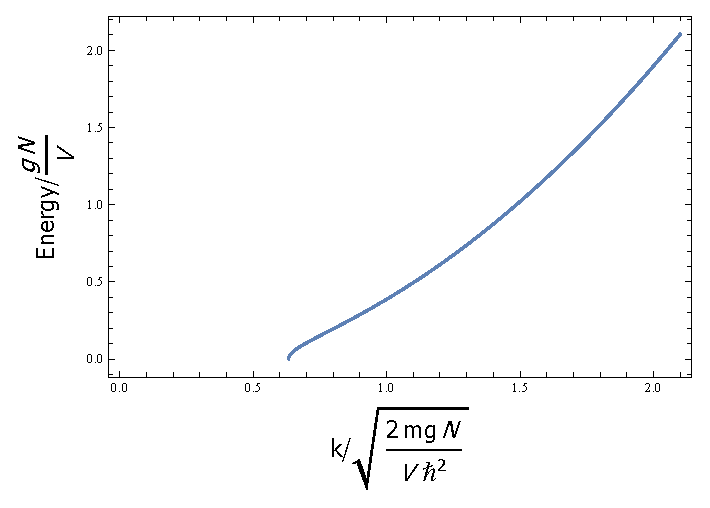
\includegraphics{Note for review_gr2.eps}
%\caption{Figure 3. This plot shows the dissipation relationship for attractive Bose-system.}
We find no excitation for small $k$, which means ground state has non-zero momentum, violating our assumption that condensate stay at $k=0$.
Thus, this result actually tells us that this attractive Bose-gas can not exist stable. We will return to this point later, when we talk about the ground state energy of this Bose system and also for double BEC case.

\subsection{Ground state and LHY correction}
Now we consider the ground state of this system. Directly take the lowest energy level from (38), we have
\begin{equation}
\begin{split}
E_{\text{GS}}=\frac{g N^2}{2V}-\frac{1}{2}\sum _{k\neq 0} \left(\epsilon _k+\frac{g N}{V}-E_k\right)
\end{split}
\end{equation}
where first term represent the mean field energy shift from {``}vacuum{''}, and second term come from quantum fluctuation (at zero temperature), i.e.
\begin{equation}
-\frac{1}{2}\sum _{k\neq 0} \left(\epsilon _k+\frac{g N}{V}-E_k\right)=-\frac{1}{2}\sum _{k\neq 0} \left(\frac{\hbar ^2k^2}{2m}+\frac{g N}{V}-\sqrt{\frac{\hbar
^2k^2}{2m}\left(\frac{\hbar ^2k^2}{2m}+\frac{2 g N}{V}\right)}\right)
\end{equation}
If you plot the term in the summation, you will find it decays with k increasing. However, if we expand it in series, we have 
\begin{equation}
\begin{split}
\frac{\hbar ^2k^2}{2m}&+\frac{g N}{V}-\sqrt{\frac{\hbar ^2k^2}{2m}\left(\frac{\hbar ^2k^2}{2m}+\frac{2 g N}{V}\right)}\\
&=\frac{1}{2}\left(\frac{gN}{V}\right)^2\left(\frac{2m}{\hbar^2}\right)\frac{1}{\pmb{k^2}}-\frac{1}{2}\left(\frac{gN}{V}\right)^3\left(\frac{2m}{\hbar^2}\right)^2\frac{1}{\pmb{k^4}}+\frac{5}{8}\left(\frac{gN}{V}\right)^4\left(\frac{2m}{\hbar^2}\right)^3\frac{1}{\pmb{k^6}}+\text{...}
\end{split}
\end{equation}
with leading proportional to $\frac{1}{k^2}$, we have divergence when sum over k to infinite. This divergence is due to the pseudo-potential with $\delta (r)$ actually does not allow calculation for large $k$, thus, we need do re-normalization to truncate this $\frac{1}{k^2}$ divergence.
Recalling the re normalized interaction $g_R$ in (27), we have
\begin{equation}
g_R=g+\frac{g^2}{V}\sum _k \frac{m}{\hbar ^2k^2}
\end{equation}
Then total energy will be
\begin{equation}
E_{\text{GS}}^R=\frac{gN^2}{2V}-\frac{1}{2}\sum_{k\neq0}\left(\frac{\hbar ^2k^2}{2m}+\frac{gN}{V}-\sqrt{\frac{\hbar^2k^2}{2m}\left(\frac{\hbar^2k^2}{2m}+\frac{2gN}{V}\right)}-\left(\frac{gN}{V}\right)^2\left(\frac{2m}{\hbar ^2}\right)\frac{1}{k^2}\right)
\end{equation}
Directly do this summation, we get the famous LHY correction
\begin{equation}
\frac{E_{\text{GS}}^R}{V}=\frac{g n^2}{2}\left(1+\frac{128}{15\pi ^{1/2}} \left(n a^3\right)^{1/2}\right)
\end{equation}
where $a=\text{Abs}\left[a_S\right]$. Now, we plot ground state energy when $g>0$
Where we can find the LHY correction is small when density is low, and only get important when $n a^3\sim 1$. These correction has been experimentally verified in strong interacting Bose System [PRL 107, 135301].
Then we plot the ground state energy with $g<0$
%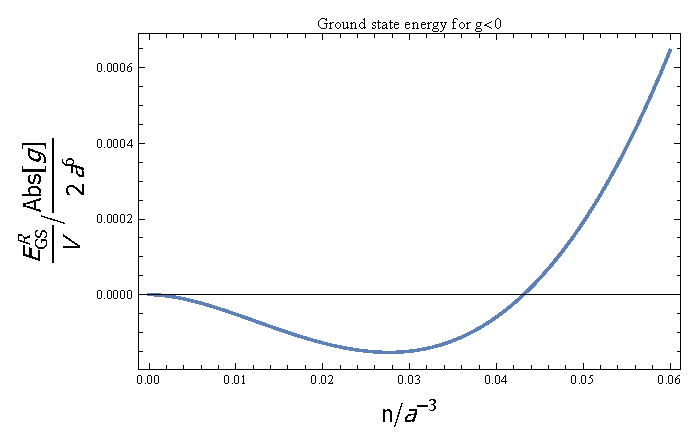
\includegraphics{Note for review_gr3.eps}
Where we find that only when \begin{equation}n a^3>0.028\end{equation}, the ground state energy increase with n increasing, which means stable ground state exist. This stability is reached due to quantum fluctuation resisting the collapse from attractive interacting, which has the same mechanics of liquid droplet in which stability is reached due to Van de Waals force. This so called LHY droplet seems haven{'}t been observed in experiment, I guess main reason is when $n a^3$ get large, the many body loss will be severe, which hides the phenomenon of droplet. We will talk more about the mechanics of LHY droplet when we considering the quantum depletion.

\subsection{Quantum Depletion and Mechanism of LHY Droplet}
Let's now consider: in a ground state of BEC at zero temperature, how many particles will not stay at $k=0$ state? The answer is just directly summation all non-zero k state in the ground state. as following
\begin{equation}
n_{\text{dp}}=\frac{1}{V}\sum _{k\neq 0} v_k^2=\frac{1}{3\pi ^2}\left(\frac{m c}{\hbar }\right)^3\propto \xi ^{-3}
\end{equation}
where $v_k$ is parameter in Bogoliubov transformation, $c =\sqrt{\frac{g n}{2m}}$ is the first sound speed in BEC, and $\xi =\frac{\hbar }{\sqrt{2m g n}}$ is healing length.
The fraction of depleted particle is
\begin{equation}
\frac{n_{\text{dp}}}{n}=\frac{8}{3\sqrt{\pi }}\sqrt{n a_S^3}
\end{equation}
we can directly read that with increasing of $n a_S^3$, more particles get out of the condensate. Meanwhile, these particles will contribute the LHY correction to ground state energy. Thus, we find that this correction beyond mean field theory actually always increase the energy and also increase {``}hot{''} particles. Moreover, if you consider the excitation spectrum for $g<0$, you can explain that the high energy excitation(short-wave)
actually cure the unstable system from long-wave-instability, which gives the formation of LHY droplet.

%For a single species condensate, with the mean-field approximation, we have its energy density propotional to \(n^2\). This is valid for low density case, which satisfies \(na_s^3<<1\). When the condition is brocken, we need a correction to further describe its behaviour, i.e. the LHY correction. From the view of ground state energy, this correction is with order of \(na_s^3\) comparing to the mean-field part, which in most case is too weak to detect. 
%这里从历史角度出发,谈历史上是如何测量LHY correction的

% discuss quantum depletion in this part
%From another point of view, i.e. how many particle stay beyond the zero momentum state, we need to introduce the quantum depletion. Similar to thermal depletion of a condensate, the quantum depletion is excited due to the inter-particle interaction. The depletion density can be written as




\chapterend


\chapter{Apparatus}
\label{Chap_Apparatus}

% epigraph
\setlength{\unitlength}{1pt}
\setlength{\epigraphwidth}{10cm}
\epigraph{工欲善其事,必先利其器。\\ A craftsman must sharpen his tools to do his job.}{--- Confucius\\ \textit{The Analects}}

% guide
In this chapter, we decribe the Na-Rb machien and upgrades we done for our droplet experiment. As most of the machine has been described by previous thesis(add ref here), we only shortly make a summary of them to make the completenees of this chapter. Then, we turn to the image system upgrades, including the optical part and machenical part. Then, we introduce the high field insitu image method for 提取 sampele's density profile reliable. Finally, we discuss several improvement such as fast coil for fast control magnetic field and improvement of the coil antenna.

\section{Overview: Na-Rb machine I}
% aim
A repeatable machien for producing stable sample with satable number, density temperature and so on, is imprtant to carry out the following experiment. So, even this Na-Rb machien has been run for longer than 8 years, there still many aspect need to improve to make the sample 状态  more stable. Besides stablity, more atom is another 追求, for many experiment, as more atom number is better for showing the many body aspect properties. So, to improve our machine to achieve more atom number is better. We persue more and cooler sample condition as possible. 

% How
Our machien start from Na and Rb dispensor. We fire our Rb dispensor every day with a relatively low  current and Na fire only once a month. The atom typically absorbed by the 腔壁 of vacuum chamber. So, we use LIAD to disabsorped the atom to the vacuum at the beginning of each shot. With the atom gradually acuumulated in 30s, our MOT capture increasing number of atoms. To avoid Rb occupating Na MOT possitin, we use a resonance light to push 一点 of the Rb MOT aside. That is out double MOT which typically can capture $10^{10}$ Rb and $10^{9}$ Na(number need check). Then, to increase its density, we apply a CMOT process to increase its density and PSD by incresing the detuning the MOT laser and increase the gradient of magnetic field. (actually, we increase no QT) Then, a molasses process to decrease the temperature of the sample then we can load the sample to QT. The QT is with gradient around 160 G/cm which is a quite deep trap as a conservation trap for capture enough number of atoms. Then, we do the evaporation cooling for Rb which using a MW to pump Rb1,-1, to 2,0 to remove the high tempreture Rb away from the trap to decrease the sampel temperature. 


\subsection{Production of Na-Rb Bose-Einstein condensate mixtures}
\subsection{Production of Na-Rb Feshbach molecules}

\section{Image system upgrades}
% why upgrade image system
The precious image system using a 100mm and 300 mm pair from Edmund optics, which can support a resolution about 4 um. This image system is build with 分立的 elemetns, which cannot move wholely. Then it is only proper for image for a single point. For our droplet experimetn, we need do the TOF for samples whcih could fall with about 2 mm. If we change the camera position, the coma will induced and worsen the resolution. So, we try to improve our resolution from two point of view: 1. imcrease its resolution. 2. make it a whole block and mount onto the eletronic stranslation stage. 

% continue why
In the following section, we will discuss the absorption image method for a dense atomic cloud. We will introduce the image scheme and discuss the number calibration method.

\subsection{High resolution image system}
% aim
As shown in section of droplet, a typical charateristic length for a droplet is about 1 um around. So, we need a resolution around this value. a typical 100mm objetive is not enough, as the airy disk of it is about 4um or around with NA about 0.1 or less.(check the value). So, to increase the NA, we need a even short focus length of the objective. A easy way is to use a microscopy with long working distance. So, we choose a MITOTOYO long working distance objective with f = 20 mm and infinite corrected, which enable us simply apply a 300mm eyepiece for direct image the atom onto camera. Notice that even the focus length of the objective is 20mm its working distance is about 36mm (check), which enable us put it just outside the cell with out block any optical path, such as MOT or optical trap. This benifits us a lot to revise our trap optics.

% about resolution
Even we use a powerful objective with resolution power about 1 um (check), one import issue is the cell wall is a thick glass with thickness 3mm(check). So, we need to check the performance of this type with 3mm window. Typically, the 3mm window will decrease the resolution, as shown in (add ref on thorlab or others). since when the focus beam go through the glass wall, light with different angle will bend by differnt  amplitude and finally they cannot converge to a single point as without the glass. This effect 影响更严重 when the NA goes higher. So, first, we try to simulate the system with zemax. As shown in Figure, two with and without 3 mm window. The resolution can be found increase to 1.5 um(check) when adding the 3mm glass. This also enouogh for our droplet experiment. So we carry out this setup.

% test resolution
Before put it online, we first test its resolution offline, with a USAF1951 target and 2um pinwhole to get a rough resolution of the image system. As shown in Figure (add), The image system with and without shows a different clearence for the target. however in both case the target is clear. Then, we measure the 2mm pinhole to get a arry partain for fitting out the real resolution value of the system. As show in Figure, the array disk is with lots of concentric rounds. by simply fitting the parttern iwht airy function, we get the resolution for Na and Rb is 0.6 and 0.8 um (check). So we now we have a high resolition and comeertial and cheap image system. 

% High-field image scheme
\begin{figure}[hb]
\begin{center}
\includegraphics[width = 0.8\linewidth]{figures/image_system.pdf}
\end{center}
\caption{image system}
\label{image_system}
\end{figure}

% coma and translation stage
As we will do TOF for sample for several mm, which could decrease the image resolution. This can be shown be Zemax by a tilted angle of input light. As Shown in Figure.(add) As we use a high magnification iamge system with rather short focus length about 20 mm, this could make its field of view quite small. So, we need to move the whole image system with the movement of atom free-falling. So, we make a compact image system and mount it onto a translation stage controlled by computer. The translation stage is mounted vertically on a 2-axis hand tuned translation stage. Its 型号 is (check), with a resolution 1um (chekc) and repitability 1um(check). We use a arduino board for drive it. finally, we can change the position of our image system at will shot by shot.

\subsection{High magnetic field absorption image}
% aim
To probe the droplet without 失真, we need the probe method reliable which means the method can recover the density profile of the sample as real as possible. Since a typical droplet sample has OD above 50 for Rb and 10(check) for Na, a typical absorption image method cannot be used dirrectly. That is because absoption image's SNR is limited when the sample OD is too high. As plotted in Figure(add), a typical probe intensity can only support OD smaller than 3 (check). With increasing the probe intensity to achiece the saturation absorption image, one can increae the thereshold of OD to probe. However, higher intensity could cause several problems(does high intensity really help for increasing the SNR of sample?) first is calibration could be hard to do or cause large error?(check) second is high intensity image for a high density sample could also induce the effect about high OD which cause non-real of the sample profile. 

% High-field image scheme
\begin{figure}[hb]
\begin{center}
\includegraphics[width = 0.8\linewidth]{figures/High-field image scheme.pdf}
\end{center}
\caption{350 G high field image scheme}
\label{High-field image scheme}
\end{figure}

% How
Thus, a typical method is to first decease the sample's density however keep its profile then do the absorption image, i,e, the partial pumping method for absorption image. A typical way is pumping a small portion of the sample to the image transition by MW or by light. As shown in Figure(add), our sample is 处在 F=1 and mF=1 state which is non reacting with the absortion light. Then, we use a pumping laser to pump the state to p state with F'=2 and F=2 state then with 自发辐射,we accumulate the atom on F=2, mF=2 state and then use the cycling transiton from this state to F=3, mF=3 state to do the absorption image. Here the pumping can also be done by the MW pulse. However a typical MW can only have a Rabi freq less than (check) 10kHz, which could comsume 100us or even longer time to apply a pi pulse. This could make the sample's shape change a lot when we probe it by the image light. So another requirement is to use a shorter pump pulse as better. So, we choose to use the pumping laser, however without using it on resonance, we make it a large detuning and also make it a high intensity. This could make sure even for a very dense sample each layer of the sample could feel around the same intensity which avoid the 不均匀性 of the saturation effect. As plotted in the Figure(add), For xxxx.... (add discription of figure here) (这里描述pupming 光为什么采用这种detuning 和power)Fianlly, we can partial pumping a small portion of the sampel to 2,2 state which can be detected directly. The pumping ratio can be controlled by the duartion of the pumping laser. As shown in the following Figre, a typical pupming fraction as a fuction of duration is ploted. We can see that for the first several tens of us, we have a almost linear puping speed(check) and after 50us(check) we have a saturation effect. This saturation effect is used to calibration latterly. For our experiemtn, to decreae the OD to 个位数sclae, we typical using a detuning 200-300(check)MHz and pumping only several us to achieve a portion less than 10 per cent. Then a typical low intnsity absorption image can afford it.

% partial_pumping
\begin{figure}[hb]
\begin{center}
\includegraphics[width = 0.8\linewidth]{figures/partial_pumping.pdf}
\end{center}
\caption{partial pumping}
\label{partial_pumping}
\end{figure}

\subsection{Atomic number calibration}

%aim
As we want to not only measure the size of the sample but also the number of sample to get the critical number of the droplet. So, a reliable recovery of its number is important. This need a carefully calibration of the sample's number. As fomulated (add) the main parameters is the alpha which describe the ratio between effective saturation intensity and the calculated saturated intensity I0, or the ratio betweent he effective cross section and the sigma0. (need restate) 
% not finished

% Image_beta_calibration
\begin{figure}[hb]
\begin{center}
\includegraphics[width = 0.8\linewidth]{figures/Image_beta_calibration.pdf}
\end{center}
\caption{Image_beta_calibration}
\label{Image_beta_calibration}
\end{figure}





\section{Fast magnetic field control}
\subsection{Fast-B coil design and driver}
% why we need fast-B coil
As we mentioned in the section about Feshbach resoannce, by tuning magnetic field we can easily control the scattering properties of atoms, i.e. the interacrion strength. In the precious set-up, we use a large Helmhotz coil with about 90(check) turns. The inductance of the coil is typically 2 mH(need check), which is a very large one with long time contants. (find a better way to describe here). So, even with driver with 100V(check), we will have a rising slope with 1ms(..), which is not fast enough for our requirement to control the interaction. Our request is depend on the time scale of the research object. For example, a typical BEC with as of 100 a0 order will have time scale less than 1 ms. Thus, to control the interaction fast we need about time scale 10 us or even faster. Then we can make sure the sample's size of other paraters changing much slower than the interaction changing.

% What is fast coil and how to build one.
So, with the above request, we need to build another coil which can generate a small but fast magnetic field. The limitation is inductance of the coil, so we reduce its winding to as few as possible. However, with fewer tunes the magnetic field it can generate all declines. So we need make a trade off here. As plotted in the following graph. we can find that their is a best tunes to generate the B-field we want. (Add Figures here) Also, to generate larger magentic field, we put it as close as posible to the cell. Finally, we choose a Helmhots coil with 6 turns in each set. The set-up with Main Feshbach coil is shown here. To adapt our previous large coil. we design a holder made of 聚酰乙烯,查一下是什么。and the holder winding with fast coil is steaked into the 2 inch optical path for MOT beam. 

% current driver and its test data
To driver this fast coil, we need a current driver which can generate fast change of current, so with Lintao's help, we design a fast coil driver with several group of JFET for fast turning on-off and also make a precision control of the current with very few leaking current. The driver schematic can be found in the appendix.C(add here)

% coupling of fast coil and main coil
As shown in JILA's thesis, now, we need to consider the coupling of the fast coil and the main coil and the environment. Since, these coupling will cause oscillation and jiggle when quenching the current in the fast coil. As modeled by the 集总 elements, as shown in figure. (Add figure). The coupling from the main coil and fast coil can be viewed as ... and environment as ... Finally, we have a tested quenching for fast coil.



\subsection{Dynamic compensation for induced and eddy current}
% Why we need dynamic compensation
There are two reasons for us to do the dynamic compensations, first is the coupling of fast coil and main coil and the environment will cause a jigger when we quench the current of the fast coil. To avoid this jigger, we 


\section{Other Technical Issues}
\subsection{Magnetic field gradient compensation}
%Why we need to compensate the B-field gradient 
As mentioned before, we use a pair of Feshbahc coil to generate large bias magntic field to control the Feshbach resonance. However, due to the imperfection of the coil, such as assymetry of each up and down coils and distance not coincident with the Helmhotz coil, the magnetic field typically has a gradient and/or curvature onto the atom. This effect can be easily detect by free-falling of atom in high magnetic field. If one find that the accelaration of the atom is deviated from gravity accelaration, there must be the gradient. Another evidence is the MW (rf) spectroscopy for a elongated sample which could detect the gradient on the horizontal direction. As shown in Figure, we free-fall Rb or Na under high magnetic field, and the accelaration is shown to be differnt from gracity, thus, in our set-up this effect could affect a lot when doing the following experiment with free-falling method. (give more number) 

% What is our gradient looks like?
Before talking about canceling this gradient, we first try to measure it. The method is simple following the MW transition calibration method. We apply the MW pulse coupled the 1,-1 and 2,0 state. Then to get the spacial distribution of the magentic field, we first let the atom free-falling, then apply the MW pulse at differnt TOF. Even though the gradient will affect the position of the atom, considering the samll effect related to g, this can be neglected. Then, we get the magnetid spactial distribution as show in Figure. We can see that there is not only a gradient of the magnetic field but also does the curvature. By a simple quadratic cruve fitting we get the curvature about 1xxx \(G/cm^2\) and an average gradient about xx G/cm. One thing need to be notice here is what we measrued is only the magnetic field gradient on vertical direction, which is the mainly contribution in our case. As we can see in the horizontal direction the accelaration is even much lower than that in veritical direction which infer that this gradient should comes mainly from the wrong distance of the Helmhotz coil.

% How to compensate the grdient and cuvarture
As it is hard to compensate the full of the curvature since to compensate the curvature we need fully recover the helmhotz condition which need much larger magnetic field compare to the several hundred gauss magnetic field. So, to 妥协性质地 solve the question we meet, we degenerate to compensate the avarage gradient to zero inside the interesting TOF we care. So, we can just add a another magnetic gradient on the vertical direction and to change the value of this gradient to find the best compensate point. For the first test, we simply use the half of our up and down shim coil (e.g. up coil). As shown in Figure, we can generate a inversely direction gradient oppposite to the main coil. Then, we simply change the current of the shim coil and test the accelarion of the atom, to find the compensation point. As the dipole moment of Na and Rb is quite different, we can also find the intersect point of them which represents zero average gradient compensation point, as shown in Figure. Finally, we tune the shim coil to the current at the in tersrct and remeasrue the magnetic field with MW spectroscopy method and compare the result with previous non-compensation one as shown in Figure. It is obvious the mean graditn is reduced a lot however the curvature is still there. The compensated gradient and curture is about xxx \(G/cm^2\) and \(xxx G/cm\) now which should be enough for observing BEC mixture free-falling. 


\subsection{Microwave full-wave loop antenna}
% Why we need to build the 2.57GHz and 7.5GHz full-wave loop antenna
As described in Section.xx, the internal states of atom can be controlled by electromagnetic wave. Typically to drive transition between two different hyperfine states, we need use micro-wave(MW) which typical has wavelength about 0.3 m to 3 m, i.e. 300MHz to 300 GHz for frequency in vacuum. For Na and Rb atom, the hyperfine splittings are 1.7 GHz and 6.8 GHz at zero magnetic field. When magnetic field increasing to 350 G (since we typically use the 347 G Feshbach resonance to control the inter-species interaction), the splitting between F=1, mF=1 and F=2, mF=2 states are 2.6 GHz and 7.5 GHz for Na and Rb separately. Thus, we need an antenna which can work well at these frequency. Here, "work well" commonly has two meanings: one is the antenna's standing wave ratio (SWR) is approaching 1, which means it can transmit more power to emitting as EM wave instead of reflecting them back to the power amplifier. Secondly, we need the atom feel the largest amplitude of E-field because the transitions between different F-state is mainly connected be electron dipole, i.e. an electrical dipole transition.(here, need more carefully check) So, the antenna's position, including its distance to atom and its direction angle are both critical to maximum the utility of the antenna. We can define the efficiency fot the above two process as $\mu_trans$ and $\mu_anta$, and the total efficiency is just the multiplication of them.

% talk about near-field and far-field difference
A commercial antenna is typically designed to work well at far field. The radiation power declines inversely proportional to the distance. Thus, in order to increase the power received by atom, we need to put the antenna as close to the atom as possible. However, this renders the radiation felt be the atom turns to be near-field instead of far-field. As depicted in Figure, the electric and magnetic field line (OK?) of a dipole antenna is plotted as blue and red separately. At a large distance of the antenna, the electric field line is almost perpendicular to the \(\hat{r}\) direction. However, when getting closed, it shows more portions to the \(\theta\) direction. This tells us that near-field electromagnetic field of antenna behaves quite different from its far-field one. At far-field region, both electric and magnetic field lines are perpendicular to the Poynting vector, which shows its radiation properties. However, the near-field cannot be treated as a radiation, instead, we typically treat it as "quasi-static" field. A quasi-static field means the distribution of EM field is the same as it in electrostatics, except a oscillation in magnitude with \(e^{i\omega t}\). In engineering, these study is important to wireless-charging, proximity sensors and so on.

% what previous one done, and what's the problem of it
Previously, we use horn antenna for Rb MW transition at 6.8GHz. (add reference here) The distance between horn and atom is about 10-15 cm (check and measure the number). Problem to put the antenna closer to the atom is its huge size which could block the optic path and its metallic body could disturb the strong magnetic field of large Feshbach coil causing a gradient on atom. So the nearest position we can put is about (10 cm) and the measurement Rabi frequency of Rb 1,1 to 2,2 transition at 350 G (7500 GHz) is less than 10kHz (check the number) with a 40 W power amplifier. The correspondents half-\(\pi\) pulse duration is about 50us (check number) which is too long for most of our experiment such as high magentic field image or too weak for dissociating the FR molecule. Thus, we need upgrade it to enhance the Rabi frequency.

% How to improve? what is full-wave loop antenna?
So, a naive solution is try to put the antenna as close to the cell as possible and try to shrink its size smaller and thinner. Therefore, the loop antenna will be a proper choice. A loop antenna is just a simple loop connected to the signal generator. However, for our case with frequency at 2.6 GHz and 7.5 GHz, The wavelength is around several cm to tens of cm. This is comparable to our coil size, which could introduce severe problem on impedance matching. A common solution is making the perimeter of the loop antenna just a full wavelength, which called the full-wave loop antenna. As shown in Figure (add figure), xxxx. when the scale of antenna is closed to wavelength, the distribution of radiation becomes quite different to those samll-loop antenna. This can be explained by a simplified picture, as shown in Figure. at the 接头地方和正对面 current changes with largest amplitude, and there placed two nodes at the quarter wavelength place to the 接头处。However, for small-lopp antenna, the current almost have same phase on the whole coil. Therefore, they have different patterns shown in Figure.

% How the antenna works?
According to the near-field quasi-static EM field theory, we can write down the EM field as following:
\begin{equation}
    E...
\end{equation}
Then, we can plot the radiation power as function of distance to the center of the loop coil, as shown in Figure. The maximum radiation appears at \(\lambda/4\) away from the plane of coil. And actually, the power at the center of coil is zero, which is in opposite to the case of a small-loop coil. For our case with f=2.6GHz, the wavelength is about 12 cm and we place the coil 3 cm away from atom to achieve the largest power. For the 7.5Ghz case, we use paramter about 4 cm coil loop, however we cannot put the coil 1 cm away from the atom since the cell has a size of 2cm, so 综合考虑optical path and power, we put the tiny coil at the side of cell with a 45 degree angle and distance to atom about 3 cm. 

% Set-up and impedance matching
After preparing the coil, we set up the standard MW power amplifier circuit for it. For the 2.6Ghz one, we use (link) from Taobao, and for the 7.5 Ghz one, we use .. from ... Before the amplifier we add a switch controlled by TTL signal and finally the signal generator is SG386. The key point to increase the efficiency from power amplifier to the coil, i.e. \(\eta_{trans}\), we need carefully consider the impedance matching from the transmission wire to eh loop coil. As shown in Figure, we demonstrate several full-wave loop antenna with different shapes. They have different impedance, the ideal one is the rectangular with aspect ratio 1:2, which just have 50 Ohm impedance. However, for our case with round shape, we have the coil with 133 Ohm. our transmission line and power amplifier are all 50 Ohm, so we need to do the impedance matching. Typical we can use a baloon, to simplify we use a 75 Ohm transition line to enhance the transmission rate. As shown in Figure, the signal can be reflected at the boundary of two lines with different impedance, and from 50 ohm to 75 Ohm wire and from 75 ohm to the 133 ohm coil, there exist two reflection wave. If we choose the length of the 75 Ohm line, we can cancel the reflection by superposition two of them. 

% How detail the impedence mathcing works
要配上公式和图片解释这个事情

% Test of the coil
Even though now we know how long the q-section line should be, we still need to do the off-line test for its performance, because a several cm length is to short to allow several uncertainty such as length uncertaainty and 衔接 place different impendence. These imcomplete can cause the phase of replectiong wave shifting and decline the effect of impedence matching. Therefor, we build a series of coil with different length of its q-section, and measrure its return loss rate by a directional coupler. As shown in Figure, we send the siganl into the outpur port of a coupler and the refleting wave from the antenna (connecting on the input port of coupler) will coupled a small portion in to the coupled port and detected by an analyser spectrum. By calculating the reflecting power and injection power, we plot the return loss rate as a function of the length og the q-section line. We can see the period does refer to the half of wavelength and there is a shift which could be attribute the imperfection of q-section line. By fitting with a sine function, we extract the 周期,shift 等等,在列表里。 So, We can now build the coil with lowest return loss for covering our usage frequency.

% Online test
Finally, we put the coil onto the atom cell. First, we test the transmission rate of the coil online to make suere the impedance matching works well, since the offline test with an enviroment open, however the online environment is full of different metals around the coil which could change the boundary condition and shift the impedance of the coil. So, we use the same mathod to test the transmision rate of the coil as shown in Figure. The bandwidth is about xxx MHz. Then, we test the Atomic Rabi frequency to measure the final performance of the coil. We apply the MW pulse for Na at 350 G and get the rabi frequency at different freq or detuning?. As shown in Figure, we test the saturation power and get a Rabi maximum to about 100kHz(check the number). This could allow us to make a pi pulse within 10 us which is enough for most case such as optical pumping in high field and also for MW spectroscopy??.

% about 6.8 7.5Ghz coil
By comfirming the 2.6 GHz coil can work, we turn to use build the 7.5 GHz coil, which could increase the Rabi freq for Rb at high field too. So, we build a similar coil with parameter about 4 cm and its q-section about xx cm, this coil is rather too samll even to put it onto the cell, because it will definitely block some part of the MOT beam. So, finally, we decide to sacrifies some power to put the coil a little bit further away from the coil, i,e, at the corner of the cell, whcih increase the distance of the coild to about 3 cm. Best working distance for the 7.5 Ghz coild should be \(\lambda/4\), i.e. 1 cm, so for 3cm distance we get a power about 1/3 compare to the maximum one (need check number). 总的来说,最后test of the rabi freq is about 100kHz, which recover the previous horn antenna performance. which could allow us to remove the horn antenna (even the coil is working on resonace at 7.5 GHz, when 6.8 Ghz it still can work with a transition rate about \(xxx\%\), so for a typical MW evaporation whichi only consumpted very small power 是足够用的了)

% https://www.everythingrf.com/community/what-is-the-difference-between-a-monopole-and-dipole-antenna
\begin{figure}[htb]
\begin{center}
\includegraphics [width =0.5 \linewidth]{Apparatus-EM_field_antenna.pdf}
\end{center}
\caption{}  
\label{antenna_EM}
\end{figure}


\begin{figure}[htb]
\begin{center}
\includegraphics [width =0.7 \linewidth]{Apparatus-loop_antenna_retrun_loss.pdf}
\end{center}
\caption{}  
\label{antenna_return_loss}
\end{figure}

\begin{figure}[htb]
\begin{center}
\includegraphics [width =0.7 \linewidth]{Apparatus-measure_SWR.pdf}
\end{center}
\caption{}
\label{SWR_measure_method}
\end{figure}


% How to build the 

\chapter{Precision characterisation of a Feshbach Resonance}
\label{Chap_Feshbach}

% epigraph (done: 2021年8月19日13:15:22)
\setlength{\unitlength}{1pt}
\setlength{\epigraphwidth}{11.5cm}
\epigraph{In physical science a first essential step in the direction of learning any subject is to find principles of numerical reckoning and methods for practicably measuring some quality connected with it. \cite{thomson_2011}}{--- William Thomson, 1st Baron Kelvin \\ \textit{Electrical Units of Measurement (1883)}}

\section{Overview}
% Introduction and purpose (done: 2021年8月19日13:19:11)
This chapter presents our precision calibration of a Na-Rb Feshbach resonance at 347.64 G. The purpose of inserting this chapter before discussing the droplet experiment is to require a precision map of the scattering length (actually not only Na-Rb but also Na-Na and Rb-Rb) as a function of the magnetic field. This narrative order is convenient for discussing the droplet experiment; however, the research in chronological order is tortuous as described in Sec. \ref{sec:intro-overview}. I learned my lesson that one should not trust any unverified data. Previous measurements of Feshbach resonance(FR) parameters of Na and Rb, by three-body-loss (3B-loss) spectrum or associating method, both encountered intrinsic systematic errors, such as thermal averaging or shifting \cite{Bartenstein2005, Zurn2013}. Due to the 
high sensitivity of the droplet phase diagram, we need the scattering length map as accurate as possible. So, we implemented the dissociation method to refine the results of FR parameters at 347.64 G resonance. In the rest of this section, we will introduce what Feshbach resonance (FR) is, discuss the previous measurement results, and finally offer the arrangement of this chapter.

% what is a FR and why use FR (done: 2021年8月13日12:45:54)
Feshbach resonance as a powerful toolbox plays its essential role in cold atom experiments. With this nob, we can tune the interaction between atoms by applying an external field. Thus, it is used to explore the few-body (or many-body) physics and form molecules that open a new field in ultracold physics. Feshbach resonance requires two channels to couple to each other. One is the open channel (or entrance channel), with which collision can produce atoms, i.e. the energy of the collision pair is larger than the asymptotic energy of the channel. Another is the closed channel which offers bound states with the set energy instead of scattering state\cite{RevModPhys.82.1225}. When the energy of one bound state in the closed channel approaching the open channel threshold (typically set to be 0), the resonance happens. Near the resonance $B_0$, the two-body scattering length is approximate as
\begin{equation}
a(B) = a_{\rm bg}\left(1+\frac{\Delta}{B-B_0}\right),
\label{FR}
\end{equation}
where $a_{\rm bg}$ is the slowly varying background scattering length, and $\Delta$ is the resonance width. By simply scanning the magnetic field, the scattering length $a$ and thus the effective two-body contact interaction can be changed from repulsive (for $a > 0$) to attractive (for $a < 0$). The capability of manipulating the interaction strengths has been playing a vital role in the study of exotic physics such as the controlled collapse~\cite{donley2001}~or soliton formation in Bose-Einstein condensates (BEC)~\cite{Khaykovich2002,Strecker2002}, the BEC-BCS crossover in quantum-degenerate Fermi gases~\citep{PhysRevLett.92.040403,PhysRevLett.92.120403,Bartenstein2004,Bourdel2004}, and more recently the formation of dilute quantum droplets~\cite{petrov2015,ferrier2016Observation,cabrera2018quantum}. In addition, FRs are used to associate atomic pairs and form weakly bound Feshbach molecules (FMs)~\cite{Kohler2006}. Combined with a subsequent two-photon Raman process, this has led to the creation of long-sought ultracold ground-state molecules~\cite{ni2008,Takekoshi2014,Molony2014,Park2015,PhysRevLett.116.205303,VOGES2020}.

% Na-Rb FR previous measurements (done 2021年8月19日13:50:52)
The typical way of tuning the scattering length by an FR in the cold atom experiment is to control the magnetic field. When the magnetic field is tuned to the vicinity of the resonance, we have a large scattering length, thus can increase the two-body collision rate. This method enables us to enhance the three-body loss rate \cite{wang2013observation}, and by scanning the magnetic field, we can obtain a loss dip (as shown in Fig. \ref{FR_loss}). This phenomenon can be used to characterize an FR directly at first glance. By a simple Gaussian fitting to extract the peak, we obtain the resonance position. The problem of calibrating an FR by this method mainly comes from the existence of lots of Efimov states near the resonance. These three-body bound states render a severe three-body loss and then broaden or shift the measurement of resonance position \cite{RevModPhys.82.1225}. Later in 2015, \cite{wang2015formation} used the association method to calibrate the 347 G and 478 G Na-Rb FR again. However, the asymmetric associating spectrum still reveals the thermal broadening and shifting, leading to inaccuracy measurement of FR parameters \cite{Bartenstein2005, Zurn2013}.

% Show a figure for one FR loss spectrum (done 2021年8月19日13:39:31)
\begin{figure}[htb]
\begin{center}
\includegraphics[width = 0.5\linewidth]{FR_loss.pdf}
\end{center}
\caption[One example of loss spectrum of Feshbach resonance.]{shows the loss spectrum of one Feshbach resonance of Na$\ket{F=1,m_F=0}$ and Rb$\ket{F=1,m_F=0}$.}
\label{FR_loss}
\end{figure}

% Introduce the dissociating method (done 2021年8月19日14:16:11)
Thus, in this Chapter, we use the most accurate method, i.e. the dissociating method, to calibrate the FR of Na and Rb at 347.64 G. To obtain an accurate map of scattering length, we need the knowledge of the molecular bound state. Recalling the discussion in chap. \ref{Chap:theory}, when we talk about quantum scattering, we typically use a pseudopotential to substitute the real complex interaction potential. However, we have to go back to the complicated real potential to obtain its scattering properties before having the scattering length. Then, an accurate map of the molecule potential is essential. Historically, people use the hot molecule to get the spectrum and then inversely deduct the potential curve \cite{}. However, this spectrum is typical only for deeply bound molecule states, which contains little information about the weakly bound states and thus the Feshbach resonances. However, our experiments need the scattering length near a Feshbach resonance, related to shallow bound states near or approaching zero when the external magnetic field is tuned across specific values. Thus, similar to the associating method, our goal is clear that we need a method to obtain these bound states energy accurately. However, to avoid the systematic error in the associating method (as shown in Fig. \ref{FR_asso}), we first form a pure molecule sample and then dissociate. Thinking in the coordinate of one molecule, one would find that this dissociation process can avoid thermal effects and thus improve the measurement accuracy. After obtaining the information of bound states, we can fit them by the coupled-channel calculation to get the Na-Rb potential. Finally, we achieve the accurate scattering length map as a function of the magnetic field. 

% Show a figure of association spectrum (done 2021年8月19日15:54:40)
\begin{figure}[htb]
\begin{center}
\includegraphics[width = 0.9\linewidth]{FR_asso.jpg}
\end{center}
\caption[Association spectrum of Na and Rb near 347.64 G. (Image from \cite{wang2015formation})]{Image from \cite{wang2015formation}. (a) and (b) shows the Na and Rb residue signal when doing the associating of Feshbach molecules. The dash-dot line shows the association limit, which corresponding to the zero-energy of the bound state. For a magnetic field less than the threshold, there are still association signals indicating the thermal effect. These thermal shifting and broadening smoothen the kink at the associating limit.}
\label{FR_asso}
\end{figure}

% arrangement of this chapter (done 2021年8月19日16:08:42)
The rest of this chapter is arranged as follows: Sec. \ref{sec:cali_FR} describes the method of dissociation measurement of FR molecule binding energy. Then, we apply the coupled-channel (c.c.) calculation fitting the data to obtain an accurate molecule potential curve. Finally, we achieve an accurate scattering length map. In Sec. \ref{sec:FR_spec_more}, we present ten more Feshbach resonance loss spectrums with different spin configurations of Na and Rb. They are compared to a c.c. calculation. We measured most elastic resonances and some of the inelastic, which process imaginary part of scattering length. This information can be used as a map for further exploration of a variety of Bose mixtures. Moreover, in the second part of Sec. \ref{sec:FR_spec_more} we demonstrate c.c. calculations for Rb-Rb and Na-Na both in $\ket{F=1,m_F=1}$ states. We find that the Na intraspecies interaction shows a very smooth variation from 54.5 $a_0$ (at 0 Gauss) to 64 $a_0$ (at around 900 G). This renders our estimation of Na-Na intraspecies scattering length shift about $10\%$ in the droplet paper \cite{guo2021leehuangyang}, from 54.45 $a_0$ to 60.05 $a_0$.

\section{Na-Rb Feshbach resonance at 347.64 G}
\label{sec:cali_FR}

% Method overview (done 2021年8月19日17:03:40)
This section\footnote{Announcement: most materials in this section is from our paper \cite{guo2021tunable}, which could lead to resemblance.} reports new measurements of binding energies for the state that causes the FR near 347.64 G. To reach the highest accuracy, we implement the dissociation method~\cite{Bartenstein2005,Zurn2013,Chin2005radio,Chapurin2019} to measure the binding energies. We achieve magnetic field stability at the mG level. The data are used to refine the interaction potentials for the $X^1\Sigma^+$ and $a^3\Sigma^+$ electronic states by fitting to coupled-channel bound-state calculations. We then use coupled-channel scattering calculations to obtain a highly accurate mapping $a(B)$ for the FR near 347.64~G. This has become a cornerstone for our recent experiment on the heteronuclear Na-Rb~quantum droplet\cite{guo2021leehuangyang}. 

% Method details (done 2021年8月19日17:27:49)
By applying a radio-frequency pulse to drive a bound-free transition~\cite{Bartenstein2005,Zurn2013,Chapurin2019}. The binding energy is obtained by subtracting the free-free transition energy from the bound-free transition energy. In the current work, as shown schematically in Fig.~\ref{FR_dis}(a), the FM lies very close in energy to the free atom pair. In this case, the dissociation can be driven by magnetic field modulation spectroscopy~\cite{Claussen2003,Thompson2005}. As illustrated in Fig.~\ref{FR_dis}(b), this is implemented by adding a small-amplitude oscillation to the magnetic field after the magnetoassociation. The oscillating magnetic field can be expressed as $B+A\times{\rm sin}(2\pi f t)$, with $B$ the final magnetic field that determines $E_{\rm b}$, and $A\ll B_0-B $. $B_0$ is the resonance magnetic field and $f$ is the modulation amplitude and frequency. Dissociation starts to occur when $f$ matches $E_{\rm b}/h$. For $f > E_{\rm b}/h$, the excess energy is converted to kinetic energy of the free atoms as $E_{\rm k} = hf - E_{\rm b}$. Due to the variation of the bound-free Franck-Condon factor with $E_{\rm k}$~\cite{Chin2005radio}, the dissociation spectrum is typically asymmetric and broad with respect to $f$.

% section outlines (done 2021年8月19日17:27:43)
In the rest part of this section, we first detailedly describe experimental measurement. Then, after obtaining the binding energies, we demonstrate the coupled-channel modelling for fitting. Finally, we compare the new calibrated parameters of Feshbach resonance at 347.64 G to the previous measurements.

% dissociation method and time sequence (done 2021年8月19日17:28:20)
\begin{figure}[htb]
\begin{center}
\includegraphics[width = \linewidth]{FR_dis.pdf}
\end{center}
\caption[Time sequence for measuring binding energy of Feshbach molecules]{Measuring the binding energy of a Feshbach molecule with magnetic field modulation spectroscopy. (a) The binding energy of the FM is $E_{\rm b}$. An oscillating magnetic field can drive a bound-free transition. (b) The FMs are first created by ramping the magnetic field across $B_0$. After the magnetic field is stabilized to its final value, a small-amplitude sinusoidal oscillation at frequency $f$ near $E_{\rm b}/h$ is added to dissociate the FMs and measure the binding energy. See the text for a more detailed description of the magnetic field ramping procedure.}
\label{FR_dis}
\end{figure}

\subsection{Measurement of the Na-Rb Feshbach molecule binding energy}

% produce atom to molecule (done 2021年8月19日17:47:03)
Our experiment starts from an optically trapped ultracold mixture of $^{23}$Na and $^{87}$Rb atoms, both in their lowest hyperfine state $\ket{F = 1, m_F = 1}$~\cite{wang2013observation,wang2015formation,jia2020}. Magnetoassociation starts from an initial magnetic field of 350 G, just above the FR at $B_0 = 347.64$ G. The magnetic field is ramped down across the resonance to form FMs, and then to 335.6 G. At this field, the FMs have a nearly zero magnetic dipole moment; this allows us to remove the residual atoms with a short and strong magnetic field gradient without losing molecules. Afterwards, the magnetic field is ramped up to a range of target values below $B_0$ for further experiments. Following this procedure, we can routinely obtain a pure sample of $^{23}$Na--$^{87}$Rb FMs with a typical temperature of 300 nK and a trap lifetime of more than 30 ms. This short lifetime is due to near-resonance photon scattering by the 947 nm optical trap light~\cite{Guo2017,jia2020}, which is provided by a home-built diode laser system. In another experiment on $^{23}$Na--$^{87}$Rb, in which a single-frequency 1064 nm laser is used as the optical trap light, FM lifetimes greater than 100 ms have been observed~\cite{Wang2019,guo2021leehuangyang}. Nevertheless, the current lifetime is more than enough for the present work, as we need only 10 ms for magnetic field stabilization and less than 1 ms for dissociation.

% remove residue atom (done 2021年8月19日21:54:33)
To obtain a high-quality dissociation spectrum, we need a pure molecule sample. If there remain atoms inside the molecule sample, though very few, because the dissociated atoms are few, it is hard to distinguish the dissociated one from the residue one. On the other hand, this part of the atom could be associated to molecules which makes the spectrum hard to subtract information. To remove residue atoms from molecules, we need to identify them by different properties, such as magnetic dipole, mass, transition frequency. To blast atoms away, we need to obtain the acceleration of atoms as large as possible and keep the molecule unaffected. The typical methods can be magnetic gradient, species-dependent optical dipole force (tune-in, tune-out trap) and resonance light for atoms. In our experiment, we originally apply the magnetic gradient at 335 G, where FMs possess zero magnetic dipoles. This method typically requires 1-2 ms to separate atoms all away from molecules, which is slow. The main limitation is the slew rate of coil current due to large coil inductance. So, later we change the method: we first transfer atoms to $\ket{F=2,m_F=2}$~state by light or by MW, then use the image cycling transition to remove the atom. With the newly upgraded full-wave loop antenna, we can achieve a high Rabi frequency for Na and Rb, both up to 50 kHz. Then, a ten us pulse could transfer all atoms to the cycling transition ground state $\ket{F=2,m_F=2}$. Then, the probe light with several saturation-intensity can blast all atoms away within less than 10 $\mu$s. More details can be found in Chap. \ref{Chap_Apparatus}.

% magnetic field modulation method (done 2021年8月19日22:07:29)
The magnetic field modulation is generated by a single loop coil driven by a low-frequency high power radio frequency amplifier. The single loop coil is placed just above the vacuum cell and coaxially with the Feshbach coils so that a modulation depth of several mG can be added to the large magnetic field. The coil has a limited modulation bandwidth of about 2 MHz. The optical trap was turned off 50 $\mu$s before applying the magnetic field modulation pulse to avoid the AC-Stark shift from the trapping light. This also reduces possible systematic errors induced by mean-field shifts of both the FMs and the free atoms as the density of FMs is lowered down. The magnetic field modulation pulse duration is chosen empirically so that the fraction of dissociation is no more than $70\%$. This is a compromise for detection signal-to-noise ratio and the requirement for using the Fermi Golden rule to fit the dissociation lineshape, which is only strictly followed for weak coupling. 

% dissociation curve 
\begin{figure}[htb]
\begin{center}
\includegraphics[width = 0.95\linewidth]{FR_spec.pdf}
\end{center}
\caption[Feshbach molecule dissociation spectrum]{Feshbach molecule dissociation spectrum at magnetic field of (a) 347.371 G, and (b) 346.000 G. The red solid curves are fitted to Eq.~\ref{eq2} to extract the FM binding energies. Because of the limited modulation bandwidth of the single-loop coil, only part of the spectrum is accessible in (b).}
\label{FR_spec}
\end{figure}

% dissociation signal (done 2021年8月21日20:22:49)
The dissociation signal is detected by absorption imaging of the fragmented $^{87}$Rb atoms. Fig.~\ref{FR_spec}(a) shows several examples of dissociation spectrum versus the modulation frequency $f$ for FMs from 347.371(5) G to 345.713(5) G. Here the magnetic field is measured with radio frequency spectroscopy of the Rb atoms. Threshold behaviors are clearly visible in all dissociation spectra. Fig.~\ref{FR_spec}(b) shows the enlargement of 347.371 G dissociation spectrum in (a). There is no dissociation is observed for $f$ below 60 kHz. Since the dissociation process involves no moment transfer, the dissociation threshold is an accurate measurement of the binding energy $E_b$ of the FM. Above this threshold, the profile of the spectrum is determined by the overlap between the wave functions of the bound and free states. As the excessive energy $hf-E_b$ will be converted into the relative motion of the two atoms, the wave function of the free atoms and thus the bound-free transition rate changes with $f$. Following~\cite{Mohapatra2015}, the lineshape of magnetic field modulation spectroscopy can be represented as
\begin{equation}
N_{Rb}(f) \propto \frac{\sqrt{hf-E_b}}{hf}.
\label{eq2}
\end{equation}
From this lineshape, a dissociation maximum should be observed at $f = 2E_b/h$, afterwards, the signal will decay with a long tail following $1/\sqrt{f}$. The spectrum in Fig.~\ref{FR_spec}(b) follows this lineshape well. For the spectrum with $E_b>1$~MHz in Fig.~\ref{FR_spec}(a), the maximum is not reached due to the limited modulation bandwidth. 

% subtract kink point, i.e. the binding energy (done 2021年8月21日20:30:58)
To determine the dissociation threshold, we fit each spectrum with Eq.~\ref{eq2}. For partial dissociation spectra like Fig.~\ref{FR_spec}(b), we have verified with simulated data that $E_{\rm b}$ can still be determined with uncertainties less than 5 kHz. The variation of $E_{\rm b}$ with magnetic field, over a range from 0.061 MHz to 1.739 MHz, is plotted in Fig.~\ref{FR_bind} as black open circles. The error bar for each $E_{\rm b}$ is smaller than the symbol size. The uncertainty in the measured magnetic field is $\pm3$~mG. 

%%% Binding energy vs. Magnetic field (done 2021年8月22日11:34:39)
\begin{figure}[htbp]
\begin{center}
\includegraphics[width = 0.9\linewidth]{FR_bind.pdf}
\end{center}
\caption[Binding energy of $^{23}$Na$^{87}$Rb Feshbach molecules at 347.64 G]{Binding energy of $^{23}$Na$^{87}$Rb Feshbach molecules created via the FR near 347.64 G in the entrance channel Na$\ket{1,1}$+Rb$\ket{1,1}$. The black open circles are the data points measured with the dissociation method. The error bars are smaller than the symbol size. The solid red curve is from the coupled-channel (c.c.) fitting, while the thin black curve is from the universal model. Inset shows the relative residue between the experiment data and the c.c. fitting.}
\label{FR_bind}
\end{figure}

% compare association method and dissociation method (done 2021年8月22日12:05:27)
Figure~\ref{FR_asso} shows $E_{\rm b}$ for FMs that were obtained in 2015 with the association method\cite{wang2015formation} near the resonances at 347.64 G. In that work~\cite{wang2015formation}, the binding energy was fitted using the square-well model~\cite{Lange2009} with a fixed background scattering length $a_{\rm bg} = 66.77a_0$. This value of $a_{\rm bg}$ was obtained from the coupled-channel modelling of the several Feshbach resonances observed with atom-loss spectroscopy in 2013~\cite{wang2013observation}. However, the square-well model requires $a_{\rm bg}$ much larger than the interaction range, which is set by the mean scattering length of the van der Waals potential \cite{Gribakin1993}; this is $\bar{a} = 55.2\,a_0$ for $^{23}$Na$^{87}$Rb. This condition is not satisfied for the Feshbach resonances considered here. It is also well known that resonance positions measured by atom-loss spectroscopy are not accurate enough due to the complicated dynamics of three-body recombination. These issues all contribute to the inaccuracy of the Feshbach resonance parameters determined previously~\cite{wang2015formation}. In the following, we solve these issues with a new coupled-channel modelling of the binding energies of the FMs.

\subsection{Coupled-channel modeling and FR parameters}
\label{sec:cc}

% introduction about method of calibration molecular potential (done 2021年8月22日17:49:00)
After obtaining the Feshbach molecule's binding energy, we measure out how the highest shallow bound state energy varies with the magnetic field. This very shallow bound state is affected mainly by the shortest part and the long-range part ($C_6$, $C_8$, $C_{10}$) of the molecular potential curve. So, by the above measurement, we can calibrate the potential more precisely, especially at short and long-range since a typical molecular potential is achieved by the Fourier-transform molecular spectroscopy\cite{Pashov2005}, which mainly use the information for the deep binding bound state, i.e. middle range potential. We can achieve a more accurate molecular potential for Na and Rb by combining the spectroscopy data for mid-range and the measurement of shallow bound state for short and long-range. 

% what is c.c. calculation (done 2021年8月22日18:11:18)
Coupled-channel calculations rely on expanding the total wavefunction for a pair of interacting atoms in a basis set that represents the electron and nuclear spins and the relative rotation of the atoms (the partial wave $L$). Substituting this expansion into the total Schr\"odinger equation produces a set of coupled differential equations that can be solved to obtain either bound-state or scattering properties. The Hamiltonian for the interacting pair is
\begin{equation}
\label{full_H}
\hat{H} =\frac{\hbar^2}{2\mu}\left[-\frac{1}{R}\frac{d^2}{dR^2}R
+\frac{\hat{L}^2}{R^2}\right]+\hat{H}_\textrm{A}+\hat{H}_\textrm{B}+\hat{V}(R),
\end{equation}
where $R$ is the internuclear distance, $\mu$ is the reduced mass, and $\hbar$ is the reduced Planck constant. $\hat{L}$ is the two-atom rotational angular momentum operator. The single-atom Hamiltonians $\hat{H}_i$ contain the hyperfine couplings and the Zeeman interaction with the magnetic field. The interaction operator $\hat{V}(R)$ contains the two isotropic Born-Oppenheimer potentials, for the $X^1\Sigma_g^+$ singlet and $a$ $^3\Sigma_u^+$ triplet states, and anisotropic spin-dependent couplings which arise from dipole-dipole and second-order spin-orbit coupling. In the present work, scattering calculations are carried out using the MOLSCAT package
\cite{molscat:2019,mbf-github:2020} and bound-state calculations use the related packages BOUND and FIELD \cite{mbf-github:2020}. The scattering wavefunction is expanded in a fully uncoupled basis set that contains all allowed spin and rotational functions, limited by $L_{\rm max}=2$. The numerical methods are similar to those used in Ref.\ \cite{Berninger:Cs2:2013}, so will not be described in detail here.

% molecular potential structure (done 2021年8月22日18:11:15)
The interaction potential used here is based on the potential curves for the $X^1\Sigma^+$ and $a^3\Sigma^+$ states of NaRb, originally obtained by fitting to Fourier transform (FT) molecular spectroscopy~\cite{Pashov2005} and later refined by Feshbach spectroscopy with ultracold atoms~\cite{wang2013observation}. The potential curve for each electronic state, with spin $S=0$ (singlet) or 1 (triplet), has three parts: (1) a high-order power-series in the well region, which is the part best determined by FT spectroscopy; (2) a long-range extrapolation, outside internuclear distance $R_{{\rm LR},S}$, which uses theoretical dispersion coefficients and a simple exchange term; (3) a short-range extrapolation, inside $R_{{\rm SR},S}$, which uses a simple repulsion of the form $A_S + B_S/R^N_S$. $R_{{\rm SR},S}$ is usually chosen as a distance just outside the inner turning point of the potential at zero energy. For particular values of $R_{{\rm SR},S}$ and $N_S$, $A_S$ and $B_S$ are usually determined so that the short-range extrapolation has the same value and derivative at $R_{{\rm SR},S}$ as the mid-range power-series potential \footnote{This constraint was applied in the present work, but for the potential of Ref.\ \cite{wang2013observation} there are derivative discontinuities at $R_{{\rm SR},S}$.}.

% fitting to get new potential (done 2021年8月22日18:11:35)
Our goal is to adjust the interaction potential to fit the measured FM binding energies, while retaining as much as possible its ability to reproduce the FT spectra. We therefore keep the two power series that represent the singlet and triplet potential wells fixed at the fitted values of Ref.\ \cite{wang2013observation}. We also retain the long-range extrapolation in its original form, with the dispersion coefficients unchanged. We vary only the parameters $R_{{\rm SR},S}$ and $N_S$ that define the short-range extrapolations. For the triplet potential, $R_{{\rm SR},1}$ is held at its original value from Ref.\ \cite{wang2013observation}, and $N_1$ is varied; this provides sufficient flexibility to adjust the singlet scattering length and reproduce resonance positions and binding energies. For the singlet potential, however, the original value of $R_{{\rm SR},0}$ is so close to the turning point that varying $N_0$ does not allow enough change in the potential to reproduce the experimental data. In this case $N_0$ is held at its original value from Ref.\ \cite{wang2013observation}, and $R_{{\rm SR},0}$ is varied.

% add potential parameters
Here attaches the new potential parameters for Na and Rb $X^1\Sigma_g^+$ singlet and $a$ $^3\Sigma_u^+$ triplet states.
\lstset{
    backgroundcolor=\color{backcolour},   
    commentstyle=\color{codegreen},
    keywordstyle=\color{magenta},
    numberstyle=\tiny\color{codegray},
    stringstyle=\color{codepurple},
    basicstyle=\ttfamily\footnotesize,
    breakatwhitespace=false,         
    breaklines=true,                 
    captionpos=b,                    
    keepspaces=false,                 
    numbersep=5pt,                  
    showspaces=false,                
    showstringspaces=false,
    showtabs=false,                  
    tabsize=2
}
\linespread{1.0}
\begin{lstlisting}
Analytic potential energy curve for the NaRb a3Sigma+ state
(for definition of parameters see C. Samuelis et al. PRA 63, 012710 (2000)) 
-------------------------------------
Potential is given with respect to the dissociation limit which is set to 0!

For R <= 4.65 A

U(R)=A+B/R^alpha

A	-232.9656123524    cm-1
B	10710621685.47      cm-1 A^alpha 
alpha       11.492

For 4.65 < R < 11.30 A

U(R)=Sum_i[a_i*((R-R_m)/(R+b*R_m))^i]

b     -0.4700
R_m   5.60071538 A 
a_0  -203.35070852 cm-1
a_1   0.122517410860683240E+01 cm-1
a_2   0.968561681714175506E+03 cm-1
a_3  -0.167358901820848331E+03 cm-1
a_4  -0.115108986132623340E+04 cm-1 
a_5   0.538103153477437104E+03 cm-1
a_6   0.576427139041465671E+04 cm-1
a_7  -0.137759208524156093E+05 cm-1
a_8  -0.484354206699185452E+05 cm-1
a_9   0.876873287464803143E+05 cm-1
a_10  0.242372373596938676E+06 cm-1
a_11 -0.283727768851481727E+06 cm-1
a_12 -0.762367745318190078E+06 cm-1
a_13  0.433100100910781766E+06 cm-1
a_14  0.150133971696866141E+07 cm-1
a_15 -0.489081569236799405E+05 cm-1
a_16 -0.164041059210233274E+07 cm-1
a_17 -0.680259713656829204E+06 cm-1
a_18  0.665168317123337765E+06 cm-1
a_19  0.606016435356653412E+06 cm-1
a_20  0.137434664322447614E+06 cm-1
  
For R>=11.30 A

U(R)=-C_6\R^6-C_8\R^8-C_10\R^10+A_ex*R^gamma*exp(-beta*R)

C_6    0.129463596372576691E+08 cm-1 A^6
C_8    0.358980000000000000E+09 cm-1 A^8
C_10   0.130601455102733498E+11 cm-1 A^10
A_ex   0.31859846D+05 cm-1 A^(-gamma)
gamma  5.00810   
beta   2.20850 A^-1

--------------------------------
Analytic potential energy curve for the NaRb X1Sigma+ state
(for definition of parameters see C. Samuelis et al. PRA 63, 012710 (2000) 
--------------------------------
Potential is given with respect to the dissociation limit which is set to 0!

For R <= 2.7256 A

U(R)=A+B/R^alpha

A           -8490.090071421    cm-1
B           450828.6299011      cm-1 A^alpha 
alpha   4.06143861049682720

For 2.7256 < R < 11.30 A

U(R)=Sum_i[a_i*((R-R_m)/(R+b*R_m))^i]

b     -0.2100
R_m    3.64340736 A
a_0   -5030.50869783 cm-1
a_1   -0.662030723944292271E-01 cm-1
a_2    0.253807725995464061E+05 cm-1
a_3    0.929104757521979809E+04 cm-1
a_4   -0.211814748606123285E+05 cm-1
a_5   -0.284181834656136671E+05 cm-1
a_6    0.210407753693068798E+04 cm-1
a_7   -0.851968733976350748E+06 cm-1
a_8   -0.123216494098773529E+07 cm-1
a_9    0.383640579108661637E+08 cm-1
a_10   0.109125343263982777E+08 cm-1
a_11  -0.109331126199059677E+10 cm-1
a_12   0.540863749615297675E+09 cm-1
a_13   0.203930014933835602E+11 cm-1
a_14  -0.222458146577416687E+11 cm-1
a_15  -0.258727375257563232E+12 cm-1
a_16   0.419458345047378906E+12 cm-1
a_17   0.226157469213112939E+13 cm-1
a_18  -0.493156268638760059E+13 cm-1
a_19  -0.133732693094783848E+14 cm-1
a_20   0.391427433409150078E+14 cm-1
a_21   0.491914424477468672E+14 cm-1
a_22  -0.214673998282790187E+15 cm-1
a_23  -0.736821254504513125E+14 cm-1
a_24   0.806693583557253000E+15 cm-1
a_25  -0.249784752437157937E+15 cm-1
a_26  -0.198517974510287375E+16 cm-1
a_27   0.172480088271182725E+16 cm-1
a_28   0.281094984850021900E+16 cm-1
a_29  -0.441448085841028300E+16 cm-1
a_30  -0.122221795646213325E+16 cm-1
a_31   0.552071157529799900E+16 cm-1
a_32  -0.210051881065563800E+16 cm-1
a_33  -0.244906408631624500E+16 cm-1
a_34   0.238499017935224850E+16 cm-1
a_35  -0.611040299017092875E+15 cm-1

For R>=11.30 A

U(R)=-C_6\R^6-C_8\R^8-C_10\R^10-A_ex*R^gamma*exp(-beta*R)

C_6    0.129463596372576691E+08 cm-1 A^6
C_8    0.358980000000000000E+09 cm-1 A^8
C_10   0.130601455102733498E+11 cm-1 A^10
A_ex   0.31859846E+05 cm-1 A^(-gamma)
gamma  5.00810   
beta   2.20850 A^-1
\end{lstlisting}

% continuing (done 2021年8月22日18:12:09)
The shape of the curve of $E_{\rm b}$ as a function of $B$ is quite insensitive to variations in the singlet and triplet scattering lengths, represented by $R_{{\rm SR},0}$ and $N_1$. It is therefore sufficient to fit to one binding energy from each FR. For the resonance near 347.64 G, we choose the point with $E_{\rm b}/h = 0.611(6)$~MHz at 346.646(5) G, while for the resonance near 478.7 G, we choose the point with $E_{\rm b}/h = 0.400$~MHz at 478.052(10) G. The parameters $R_{{\rm SR},0}$ and $N_1$ are then adjusted so that these binding energies are reproduced essentially exactly. The resulting values are $R_{{\rm SR},0}=2.7256$~\AA\ and $N_1=11.492$. The singlet and triplet scattering lengths calculated from the fitted potentials are  $a_{\rm s} = 106.474 a_0$ and $a_{\rm t} = 68.864 a_0$, respectively. These are $0.27 a_0$ smaller and $0.24 a_0$ larger than the values of Ref.\ \cite{wang2013observation}, indicating that the triplet potential needs to be slightly more repulsive than the original at short range, while the singlet potential needs to be slightly less repulsive.

% obtain FR parameters (done 2021-8-22 18:12:32)
We use the fitted potentials to calculate the $s$-wave scattering length $a(B)$. We find that each resonance is well represented by Eq.~\ref{FR}. The parameters $B_{0}$, $\Delta$ and $a_{\rm bg}$ are obtained as described by Frye and Hutson \cite{Frye2017}, and are given in Table~\ref{tab1}. In Fig.~\ref{FR_bind}, the binding energies calculated from the universal model $E_{\rm b} = \hbar^2/2\mu a(B)^2$ using the new $a(B)$ is also shown. Compared with the coupled channel results (red solid curve), this reproduces the data only for $E_{\rm b}< 0.6$ MHz. 

% Parameters of the two low-field $s$-wave Feshbach resonances (done 2021年8月19日22:40:53)
\begin{table}[htb]
\caption{Parameters of the two low-field $s$-wave Feshbach resonances for the entrance channel Na$\ket{1,1}$+Rb$\ket{1,1}$.}
\label{tab1}\centering
\begin{tabular}{ c | c | c | c }
\hline\hline
$B_0$ (G) & $\Delta$ (G) & $a_{\rm bg}$ ($a_0$) & reference\\
\hline
347.648 & 4.255  & 76.33 & this work\\
347.64 & 5.20  & 66.77 & \cite{wang2015formation}\\
347.75 & 4.89  & 66.77 & \cite{wang2013observation}\\
\hline
478.714 & 3.491  & 71.55 & this work\\
478.83 & 4.81  & 66.77 & \cite{wang2015formation}\\
478.79 & 3.80  & 66.77 & \cite{wang2013observation}\\
\hline \hline
\end{tabular}
\end{table}

% comparison(done 2021-8-22 18:18:23)
In the present fit, the resonance near 347.64 G has shifted by about 0.08 G compared to Ref.\ \cite{wang2013observation}. The resonance near 487.7 G has shifted by more than 0.1 G. These shifts produce substantial changes in the calculated scattering lengths. Moreover, in Ref.\ \cite{wang2013observation}, the calculated scattering length was fitted using the formula
\begin{equation}
a(B)=a_{\rm bg} \left[1 + \frac{\Delta_0}{B-B_0} + \frac{\Delta_1}{B-B_1} + \dots\right],
\label{eq:FRsum}
\end{equation}
with a single $B$-independent background scattering length $a_{\rm bg}$ for all resonances. This formula breaks down when the background scattering length varies significantly between resonances. In the present work, Eq.~\ref{FR} is found to be a good local representation for each resonance, but significantly different values of $a_{\rm bg}$ are needed for the resonances at 347.64 G and 487.7 G. Such behavior can arise from many sources, including the changing spin character of atomic states with magnetic field and the presence of additional resonances not included in the summation of Eq.\ \ref{eq:FRsum}. As shown in Fig.~\ref{FR_para}, for the resonance near 347.64 G, the scattering lengths calculated with the new potential differ by about $20a_0$ from those of Ref.\ \cite{wang2015formation} in the region from 349.8 G to 350.0 G that is important for studies of Na-Rb quantum droplets. This change is significant and largely explains the discrepancies initially observed between experiment and theory in Ref.\ \cite{guo2021leehuangyang}.



%%% Binding energy vs. Magnetic field (done 2021年8月22日18:18:11)
\begin{figure}[htbp]
\begin{center}
\includegraphics[width = 0.9\linewidth]{FR_para.pdf}
\end{center}
\caption[Scattering length as function of magnetic field]{Comparison of the mapping between magnetic field and scattering length with Feshbach resonance parameters obtained in this work, using coupled-channel results directly (blue open circles) and fitted to Eq.~\ref{FR} (blue solid curve) and , and in Ref.~\cite{wang2015formation} (red dash-dotted curve) and Ref.~\cite{wang2013observation} (black dashed curve), both using Eq.~\ref{eq:FRsum}. The region of interest for the droplet experiment~\cite{guo2021leehuangyang}, marked with a vertical gray bar, is enlarged in the inset. }
\label{FR_para}
\end{figure}

% some explanation for c.c. (done 2021年8月22日18:18:55)
All the coupled-channel calculations use a basis set that includes functions for partial waves $L = 0$ and $L =2$, with the effective dipolar coupling function of Ref.\ \cite{wang2013observation} unchanged. Omitting the $L = 2$ basis functions causes shifts that are on the same level as the experimental uncertainties: the calculated resonance positions and binding-energy curves shift down by between 3 and 4 mG. It is possible to include additional partial waves, but we expect the shifts to be very small. In contrast to Ref.\ \cite{wang2013observation}, we do not include any variation of the atomic hyperfine coupling with internuclear distance.


\section{Na-Rb, Na-Na and Rb-Rb scattering length summery}
\label{sec:FR_spec_more}
% overview (done 2021-8-22 18:37:21)
Besides the Feshbach resonance at 347.64 G, different combinations of the spin state of Na and Rb possess plenty of FRs. Ref.~\cite{wang2013observation} investigated the entrance channels $\ket{m_F=1}+\ket{m_F=1}$ and $\ket{m_F=-1}+\ket{m_F=-1}$ and in total observed three $s$-wave and two $p$-wave FRs. In addition, ten more $s$-wave FRs were predicted for collisions between pairs of atoms in different $F = 1$ hyperfine Zeeman states. In this section, we report the experimental observation of several of these FRs below 1000 G in 5 hyperfine Zeeman combinations. We believe these FRs will find important applications in the future, for example, in the investigation of BEC mixtures and quantum droplets with more than two components~\cite{ma2021}. 

% some words on the Na-Na scattering length (done)
With the powerful tool, MOLSCAT \cite{molscat:2019,mbf-github:2020}, we can get more precise maps of scattering length and magnetic field. Since even the background scattering length varies when the external field changes, the value of the scattering length, especially for a finite (not low) field, should be treated with more care. Here we find that the Na-Na 1,1 state have a smoothly varying background scattering length from low field to around 900 G (near the FR). Its value starts from 54.45 $a_0$ to about 64 $a_0$. For our droplet experiment, under about 350 G magnetic field, the Na-Na scattering length is 60.05 $a_0$ which is larger about 10\% than at low field.

\subsection{Na-Rb scattering length for different spin combination}

% experiment preparation state (done 2021-8-22 18:52:27)
For simplicity, we will denote the collision channel of a pair of $^{23}$Na+$^{87}$Rb atoms by $\ket{m_F^{\rm Na}}+\ket{m_F^{\rm Rb}}$. In ref.~\cite{wang2013observation}, both the $\ket{1}+\ket{1}$ and the $\ket{-1}+\ket{-1}$ channels were investigated and in total 3 $s$-wave and 2 $p$-wave FRs were observed. As shown in Fig. \ref{FR_more}, we detect more FRs in different combinations. The experiment for this section starts from optically trapped thermal mixtures of Na and Rb both in the $\ket{-1}+\ket{-1}$ channel. The number of atoms for both species are typically around $10^5$ and the sample temperatures are about 1~$\mu$K. The atoms are then transferred to selected hyperfine Zeeman levels with radio frequency (rf) rapid adiabatic passages. For each species, the $\ket{-1}\rightarrow \ket{0}$ and the $\ket{0}\rightarrow \ket{1}$ Zeeman splittings are very similar. In addition, these splittings in different species are also very similar to each other. To avoid cascade transitions and to realize species-selective state control, the state transfers are performed at 100 G where the transitions are all different by more than 500 kHz. With this method, we are able to prepare the Na-Rb mixture in all the 9 possible $m_F$ combinations of their $F = 1$ states. Then, we ramp the magnetic field to different values and hold the samples for 50 ms before releasing the atoms from the optical trap and measuring the remained numbers of atoms. Intersperses FRs manifest as losses of atoms in both $^{23}$Na and $^{87}$Rb~atoms as a result of enhanced interspecies three-body recombination rates. As presented in Fig.~\ref{FR_more}, guided by the predictions in~\cite{wang2013observation}, we observe 10 FRs in 6 hyperfine Zeeman combinations. 

%%% figure of 10 more FR spectroscopy (done 2021年8月22日18:52:16)
\begin{figure}[htb]
\begin{center}
\includegraphics[width = \linewidth]{FR_more.pdf}
\end{center}
\caption[Loss spectroscopy of Feshbach resonance with different spin combinations]{Feshbach resonances in $^{23}$Na-$^{87}$Rb, observed by losses for atoms in the $F = 1$ hyperfine states. (a) and (b) are for the two channels in the $M_F = 1$ manifold; (c), (d) and (e) are for the three channels in the $M_F = 0$ manifold. The typical holding time at each magnetic field is 50 ms. The solid curves are from Gaussian fitting to determine the lineshape center. Error bars for the atom numbers represent one standard deviation. The large error bars for the magnetic field for the several broad loss spectra are due to less precise magnetic field control in these cases (see text).}
\label{FR_more}
\end{figure}

% implement c.c. calculation (done 2021年8月23日10:09:31)
We have carried out coupled-channel calculations of resonance parameters for both elastic and decayed resonances, using the interaction potentials obtained in Sec.~\ref{sec:cc}. The results are included in Table~\ref{fst}. For elastic resonances, the resonance positions for the lowest threshold of each $M_F$ is first located with the FIELD program~\cite{mbf-github:2020}. The FRs are then characterized using the MOLSCAT program~\cite{molscat:2019,mbf-github:2020} following the elastic procedure of Ref.~\cite{Frye2017}, which converges on the resonance position $B_0^{\rm cc}$, the elastic resonance width $\Delta$, and the background scattering length $a_{\rm bg}$. Here $a_{\rm bg}$ is a local background scattering length that is different for each resonances. In the current calculation, we have not included the spin-spin interaction, so that both the quantum number $L$ of the partial wave and its projection $M_L$ are conserved in the calculation. Since $M_{\rm tot} = m_F^{\rm Na}+m_F^{\rm Rb} + M_L$ is conserved, only closed channels with $M_F = m_F^{\rm Na}+m_F^{\rm Rb}$ the same as the colliding atoms can cause FRs.

% FR spectroscopy and c.c. calculation table (done 2021年8月23日10:11:19)
\begin{sidewaystable}[thp]
\caption[Summary table of Na-Rb Feshbach resonances with different spin combinations]{Comparison of experimental resonance positions $B_0^{\rm exp}$ with theoretical parameters for interspecies FRs below 1000 G in $^{23}$Na-$^{87}$Rb, for the nine $F = 1$ entrance channels. $L$ indicates the partial wave of the entrance channel. $B_0^{\rm exp}$ is the mean of the centers of the loss spectra for $^{23}$Na and $^{87}$Rb in Fig.~\ref{FR_more}, determined by Gaussian fitting. Error bars represent one standard deviation. The theoretical values are from coupled-channel calculations using the singlet and triplet potential-energy curves described in Sec.~\ref{sec:cc} with the latest potential parameters. $B_0^{\rm cc}$, $\Delta$, and $a_{\rm bg}$ are the theoretical position, elastic width, and background scattering length, respectively. The last column ``inel.?'' indicates whether the FR is subject to inelastic losses from spin exchange. For decayed FRs with inelastic losses, the resonant scattering length $a_{\rm res}$ and the inelastic width $\Gamma_{\rm inel}$ are also listed.}
\label{fst}\centering
\begin{tabular}{l|c|l|c|c|c|c|c|c}
\hline\hline
Entrance channel 				& $L$ & $B_0^{\rm exp}$(G)	& $B_0^{\rm cc}$(G)	& $\Delta$(G)	& $a_{\rm bg}$($a_0$) & $a_{\rm res}$($a_0$) & $\Gamma_{\rm inel}$(G)	& inel.? \\
\hline
Na$\ket{1,1}$ + Rb$\ket{1,1}$   & 0    	& 347.61(2)       	& 347.645 			& 4.258  			 & 76.328  	& & & N     \\
					        	& 0 	& 478.82(3)        	& 478.712 			& 3.495  			 & 71.548   & & & N     \\ \hline
Na$\ket{1,1}$ + Rb$\ket{1,0}$   & 0    	& 388.5(2)          & 388.577 			& 5.684  & 78.441                 &6548.8 & $-0.13617$& Y     \\
								& 0    	& 522(10)           & 524.286 			& 1.010  & 74.332                 & 12.906& $-11.634$& Y     \\ \hline
Na$\ket{1,0}$ + Rb$\ket{1,1}$   & 0   	&  	--		        & 358.078 			& <0.001  & 80.108                & & & N     \\
								& 0   	& 484.45(5)         & 484.569 			& 4.476  & 77.258                 & & & N     \\
								& 0		& 	--				& 570.441			& <0.001	& 73.784			 & & & N \\
								& 0   	& 716.97(6)         & 717.166 			& 5.593  & 72.998                 & & & N     \\  \hline
Na$\ket{1,1}$ + Rb$\ket{1,-1}$ 	& 0    	& 587(3)         & 580.686 			& 0.241  & $82.389 - 0.0072 i $  & $2.3917 + 0.87566 i$&$-16.596$& Y     \\
							  	& 0    	& 920(1)         & 913.431 			& 0.091  & $81.139 + 0.0352 i$ & $0.47768 + 0.12885 i$& $-30.861$& Y     \\ \hline
Na$\ket{1,0}$ + Rb$\ket{1,0}$  	& 0    	& 410.90(1)         & 409.810 			& 0.176  & 82.328                 & & & N     \\
    							& 0    	& 526.29(3)         & 526.548 			& 5.676  & 78.132                 &23515 &$-0.03772$ & Y     \\
    							& 0    	& 759(13)           & 768.781 			& 1.638  & 75.495                 &19.983 &$-12.373$ & Y     \\ \hline
Na$\ket{1,-1}$ + Rb$\ket{1,1}$ 	& 0    	& --		        & 419.648 			& <0.001  & 80.109                &0.25533 &$-0.34477$ & Y     \\
								& 0    	& --        		& 516.986 			& 0.003  & 79.401                 & & & N     \\	
								& 0    	& 724.38(4)         & 727.270 			& 4.870  & 76.444                 & & & N     \\ \hline
Na$\ket{1,0}$ + Rb$\ket{1,-1}$  & 0    	& --          		& -- 			& -- & --                             & & & N     \\ \hline
Na$\ket{1,-1}$ + Rb$\ket{1,0}$  & 0    	& --          		& 609.754 			& 0.416 & 80.572                  & & & N     \\
								& 0		& --				& 759.441			& 5.676 & 78.826				  & & & N \\ \hline	
Na$\ket{1,-1}$ + Rb$\ket{1,-1}$ & 0    	& 899.8(3)          & 900.317 			& -0.315 & 79.270                 & & & N     \\
								& 1    	& 954.2(3)          & 954.755 			&   &         				      & & & N     \\
								& 1    	& 954.5(3)          & 955.024 			&   &         					  & & & N     \\
\hline \hline
\end{tabular}
\end{sidewaystable}
%% END of Table

% 1+1 and -1+-1 both elastic channel (done 2021-8-23 14:58:09)
\begin{figure}[tb]
\begin{center}
\includegraphics[width = \linewidth]{FR_groupAE.pdf}
\end{center}
\caption[Scattering lengths of Na$\ket{1}$+Rb$\ket{1}$ and Na$\ket{-1}$+Rb$\ket{-1}$ elastic channels]{Both Na$\ket{1}$+Rb$\ket{1}$ and Na$\ket{-1}$+Rb$\ket{-1}$ are elastic channels. Here we only plot the real part of the scattering length since there is no imaginary part. Two resonances show in Na$\ket{1}$+Rb$\ket{1}$ channel and one in Na$\ket{-1}$+Rb$\ket{-1}$ channel. A smooth variation of the scattering length is obvious in Na$\ket{-1}$+Rb$\ket{-1}$ channel.}
\label{FR_groupAE}
\end{figure}

% about elastic channel (done 2021-8-23 14:57:59)
As shown in Table~\ref{fst} and in Fig. \ref{FR_groupAE}, Na$\ket{1}$+Rb$\ket{1}$ Na$\ket{-1}$+Rb$\ket{-1}$ are two channels with all resonances elastic, which means there is no possible for the scattering to other channels. These resonances are a pole as shown in the scattering length plot following the $1/(B-B_0)$ variation. If only considering the two-body collision, one would not have the loss peak as shown in Fig. \ref{FR_loss} or Fig. \ref{FR_more}, because increasing the scattering length only means increasing the elastic collision rate. So, the loss peaks in those measurements are the result of the three-body loss.

% group B for total M=1 (done 2021-8-23 14:51:43)
\begin{figure}[htb]
\begin{center}
\includegraphics[width = \linewidth]{FR_groupB.pdf}
\end{center}
\caption[Scattering lengths of $M_F=1$ channels]{Scattering lengths of $M_F=1$ channels, including Na$\ket{1}$+Rb$\ket{0}$ and Na$\ket{0}$+Rb$\ket{1}$. Left(right) shows the real(imaginary) part of the scattering length. For Na$\ket{1}$+Rb$\ket{0}$ channel there are two inelastic resonance with non-zero imaginary part of scattering length.}
\label{FR_groupB}
\end{figure}
% group C for total M=0 (done 2021年8月24日12:12:39)
\begin{figure}[htb]
\begin{center}
\includegraphics[width = \linewidth]{FR_groupC.pdf}
\end{center}
\caption[Scattering lengths of $M_F=0$ channels]{Scattering lengths of $M_F=0$ channels, including Na$\ket{1}$+Rb$\ket{-1}$, Na$\ket{0}$+Rb$\ket{0}$ and Na$\ket{-1}$+Rb$\ket{1}$. Left(right) shows the real(imaginary) part of the scattering length.}
\label{FR_groupC}
\end{figure}

% about inelastic channel I (done 2021年8月24日12:08:25)
When an inelastic channel is present, the states at the threshold are quasi-bound, so using FIELD is more complicated. Instead, the FRs are located by computing the scattering lengths for magnetic fields up to 1000 G using the MOLSCAT program~\cite{molscat:2019,mbf-github:2020}. Once an FR is located, the resonance parameters are then determined following the regularized scattering length or fully complex procedure of Ref.~\cite{Frye2017}. In this case, the scattering length is complex and shows an oscillation rather than a pole at resonance \cite{Hutson:res:2007}. Such a resonance is termed decayed, and the procedure generates the resonant scattering length $a_{\rm res}$ and the inelastic width $\Gamma_{\rm inel}$ in addition to $B_0^{\rm cc}$, $\Delta$ and $a_{\rm bg}$.

% about inelastic channel II (done 2021年8月24日12:09:06)
The calculation reproduces all the observed $s$-wave resonances. As shown in Table~\ref{fst}, the deviations between $B_0^{\rm cc}$ and $B_0^{\rm exp}$ are within 0.5 G for most of the elastic FRs, labelled by ``N'' in the last column ``inel?''. The only exception is the resonance observed at 410.9 G for the entrance channel $\ket{0} + \ket{0}$, for which $B_0^{\rm cc}$ is 1.1 G lower. As shown in Fig.~\ref{FR_Zeeman-BC}(b), this channel features a nearby switchover between the relative channel energies near 450 G. The four $s$-wave resonances for the entrance channels $\ket{1}+\ket{1}$ and $\ket{0}+ \ket{1}$ all have calculated resonance widths $\Delta$ of several Gauss. They should all be useful for investigating Na--Rb mixtures with tunable interactions. These resonances also have rather small calculated effective ranges, on the order of 10s of $a_0$; thus, using the scattering lengths should be sufficient for most applications.

% Zeeman energy for $M_F=1$ and $M_F=0$ channels (done 2021-8-23 10:26:28)
\begin{figure}[htb]
\begin{center}
\includegraphics[width = \linewidth]{FR_Zeeman-BC.pdf}
\end{center}
\caption[Zeeman energy for $M_F=1$ and $M_F=0$ channels]{(a) Channel energies for the manifold with $M_F = 1$ for magnetic field up to 1000 G. (b) The same for the manifold with $M_F = 0$. The energies of the channels $\ket{0}+\ket{0}$ and $\ket{-1}+\ket{1}$ cross each other near 450 G, as marked by the black open circle. For each $M_F$, atom pairs in higher-energy channels can undergo inelastic loss by spin exchange to the lower-energy channels.}
\label{FR_Zeeman-BC}
\end{figure}

% about inelastic channel III (done 2021-8-24 12:09:25)
The decayed FRs can have very different characters, depending on $a_\textrm{res}$ and/or $\Gamma_\textrm{inel}$. When $a_\textrm{res}$ is large and $\Gamma_\textrm{inel}\ll\Delta$, the resonance \emph{may} be fairly similar to the elastic case and be dominated by three-body loss. However, when $a_\textrm{res}$ is small and $\Gamma_\textrm{inel}$ is comparable to or larger than $\Delta$, the loss is more likely to be dominated by two-body loss. This looks to be the case for the resonances at 522 G for $\ket{1}+\ket{0}$, at 759 G for $\ket{0}+\ket{0}$, and the unobserved one at 420 G for $\ket{-1}+\ket{1}$. It is also true for both resonances for $\ket{1}+\ket{-1}$, but for those there is a significant \emph{background} loss characterized by the imaginary part of $a_\textrm{bg}$.

% group D for total M=-1 (done 2021年8月24日12:12:28)
\begin{figure}[htb]
\begin{center}
\includegraphics[width = \linewidth]{FR_groupD.pdf}
\end{center}
\caption[Scattering lengths of $M_F=-1$ channels]{Scattering lengths of $M_F=-1$ channels, including Na$\ket{0}$+Rb$\ket{-1}$ and Na$\ket{-1}$+Rb$\ket{0}$. Left(right) shows the real(imaginary) part of the scattering length.}
\label{FR_groupD}
\end{figure}

% about inelastic channel IV
For the decayed resonances with $\Gamma_\textrm{inel} <1$ at 388 G for $\ket{1}+\ket{0}$ and at 526 G for $\ket{0}+\ket{0}$, the calculated resonance positions $B_0^{\rm cc}$ agree with the measured resonance positions $B_0^{\rm exp}$ very well. However, deviations up to several Gauss are observed for inelastic resonances with large $\Gamma_\textrm{inel}$. These can be attributed to several factors. For the two resonances with very broad observed loss spectra at 522 G for $\ket{1}+\ket{0}$ and at 759 G for $\ket{0}+\ket{0}$, the resonance centers have large uncertainties near 10 G. In addition, in presence of the background loss, the two-body loss induced by these resonances has an asymmetric (Fano-like) profile and its measured peak is not at $B_0$. Finally, although we have not studied them carefully, some nearby intraspecies FRs in Na or Rb may also affect the measurements of the resonance positions.

% about those not observed
Several resonances predicted by the coupled-channel calculation are not observed experimentally. Most of these are very narrow ones with calculated $\Delta$ in the mG range. No resonance is found from the calculation for the entrance channel $\ket{0}+\ket{-1}$. In addition, we have not searched experimentally for FRs in the entrance channel $\ket{-1}+\ket{0}$ although the calculation indicates that two resonances should exist.

% about p-wave resonances and some comments
Table~\ref{fst} also lists the several $p$-wave FRs observed by~\cite{wang2013observation} for the entrance channels $\ket{1}+\ket{1}$ and $\ket{-1}+\ket{-1}$. As mentioned above, we have not attempted to improve the agreement between the current calculation and the experiment by including the dependence of the atomic hyperfine coupling on $R$. We note that Ref.~\cite{Cui2018}, which presented a compilation of FRs for alkali atoms calculated with multichannel quantum defect theory (MQDT), identified the resonance near 284 G as a ``broad'' $p$-wave resonance. It would be possible to perform a full-scale coupled-channel fitting to these resonances. This, however, is not pursued here as it would involve further adjustments to the potential parameters, beyond those used in Ref.\cite{guo2021leehuangyang}. In view of the inaccuracy of the loss spectroscopy compared with the measurements of FM binding energies, we believe such fitting is not currently justified.

\subsection{Na-Na and Rb-Rb scattering length}

% calculation
Besides interspecies Na-Rb scattering properties, we also study the intraspecies scattering length for Na-Na and Rb-Rb, because the droplet experiment needs all three scattering lengths. Out calculation directly send the potential file from \cite{} to MOLSCAT \cite{} and then use the molscat modular to obtain the scattering length. The Feshbach resonances for Na-Na and Rb-Rb are all far away from 347 G, where we study the droplet \cite{}. However, Na-Na scattering length varies with magnetic field very smoothly, even without resonance. As shown in Fig. \ref{FR_NaNa}, From 0 to around 800 G, we have a scattering length changing from 54.5 $a_0$ to about 64 $a_0$. For magnetic field around 350 G, i.e. the field for forming droplet sample, the scattering length for Na-Na is 60.05 $a_0$. This value is about 10\% larger than in a low magnetic field. 

% Na-Na 1,1 scattering length (done 2021-8-23 14:44:27)
\begin{figure}[htb]
\begin{center}
\includegraphics[width = 0.7\linewidth]{FR_NaNa.pdf}
\end{center}
\caption[Na$\ket{1,1}$ + Na$\ket{1,1}$ scattering length as a function of magnetic field]{Na$\ket{1,1}$ + Na$\ket{1,1}$ scattering length as a function of magnetic field. A smooth changing from }
\label{FR_NaNa}
\end{figure}

% more comments
Verifying the Na-Na scattering length value is not easy since the smooth-changing background scattering length only has about 10\% to 20\% variation. Typical methods for measuring $s$-wave scattering length, such as measurement of elastic collision rate by tracing the thermalization process\cite{} or by measuring the BEC expansion\cite{}, are all difficult and need precisely calibration of some other physical parameter (such as atomic number in the second method). These measurements are prone to have an error with 10\% to 20\%. On the other hand, the coupled-channel calculation is the most precise method and is an ab initio calculation that offers reliable numbers. So, we directly take the calculated one.

\chapterend
\chapter{Quantum droplet of hetero-nuclear Bose mixture}
\label{Chap_droplet}

% epigraph (done 2021-9-30 09:06:25)
\setlength{\unitlength}{1pt}
\setlength{\epigraphwidth}{10cm}
\epigraph{Law of physicists I: \\ Without experimentalists, theorists tend to drift. \cite{Lee:1992ui}}{--- T.D. Lee\\ \textit{History of the weak interactions (1987)}}

% Overview and structure of theory part of this chapter (done 2021-10-7 20:49:40)
This chapter discusses the heteronuclear droplets formed by the Bose-Einstein condensate mixture of Na and Rb. We first reanalyze the droplet, however, with a finite volume instead of homogeneous density distribution. This is for comparison with experiments since an actual quantum droplet we build in the experiment always has a specific size due to a limited atomic number. We make a rough estimation by analyzing the energy scales of each term. Then, continuing with the analytical solution in Sec. \ref{sec:droplet_ana}, we implement the variational calculation. We use a simple Gaussian trial function to help understand how different energy scales compete in the finite-size droplets. Its specific size mainly requires introducing a kinetic energy term (i.e. quantum pressure). In order to better understand the droplet sample, we simulate it with extended Gross–Pitaevskii equation (eGPE). In this part, we give the derivation of the extended GPE especially for the two-species BEC sample near zero MF energy region. We put the code of GPELAB \cite{ANTOINE20142969} and samples of the simulation results in the Appendix \ref{chap:eGPELAB} with more details.

% Overview and structure of experiment part of this chapter (done 2021-10-7 22:54:47)
In Sec. \ref{sec:droplet_experiment}, we experimentally study Na-Rb droplet and measure the phase diagram of liquid-gas phase transition, which is the central part of our experimental research. The experimental method is simple and straightforward. We directly let the sample do Time-of-Flight and observe the non-expansion signal. This method avoids the complexity of the optical-levitation method however need more effort to eliminate the inhomogeneity of the magnetic field. In order to cooperate with this scheme, we upgrade our system on both control of magnetic field and imaging method, referring to Sec. \ref{sec:image} and Sec. \ref{sec:fastcoil} for details. Later, in Sec. \ref{sec:LHY_gas}, we study the gaseous LHY sample. This research aims to explore the behaviour of a gaseous sample under the dominance of LHY energy instead of MF energy. This research is a supplement to the study of LHY gas by measuring the trap frequency \cite{skov2020}. After understanding the droplet formation process, we realize that the previous process of preparing droplets is far from adiabatic, which resulted in significant limitations on the sample life and the number of atoms. So we improve the preparation scheme to achieve a droplet sample with more numbers as shown in Sec. \ref{sec:mode_match}. Finally, Sec. \ref{sec:droplet_molecule} shows our efforts on using droplets to form the Feshbach molecules. Although the conversion efficiency has no improvement, we have greatly reduced the temperature of the molecules and provide a promising path for the future production of degenerate Feshbach molecules.


\section{Quantum droplet with finite size}

% overall of this section (done 2021-10-8 09:20:57)
In Sec. \ref{sec:droplet_ana}, we calculate the quantum liquid analytically, showing the mean-field and LHY energy expressions. Then we obtain the equilibrium density of the system. This calculation ignores the system's quantum pressure (kinetic energy), which means it is only proper for homogeneous bulk samples. However, in our experiments, due to the limitation of the atomic number, we currently cannot obtain a sample with a large enough number allowing us to ignore its edge. Thus, in this section, we first analyse the quantum pressure caused by the finite volume then show its influence on the quantum liquid droplet. 

% introducing energy expression
The total energy of the system consists of three parts, in addition to the interaction energy from MF and LHY, there is also the quantum pressure. The expression is as follows
\begin{equation}
\begin{split}
E_{\text{kin}}=N \frac{\hbar ^2}{2m}\int \left| \nabla \phi (\pmb{r})\right| ^2 \, dr^3\\
E_{\text{trap}}=N\int \left| \phi (\pmb{r})\right| ^2V_{\text{trap}}(\pmb{r})dr^3,\text{   }V_{\text{trap}}(\pmb{r})=\frac{1}{2}m \omega _0^2\pmb{r}^2\\
E_{\text{MF}}=\frac{g}{2}N^2\int \left| \phi (\pmb{r})\right| ^4 \, dr^3,\text{    }g=\frac{2\pi  \hbar ^2a_S}{m/2}
\end{split}
\end{equation}
where ... 什么是什么
局部而言,MF能量正比于n方,LHY正比于n 2.5 次方。动能正比于波函数变化,所以对于homogeneous的bulk sample,这一项是零。但是,考虑到边界上波函数迅速降低(里面density 有限,外面是真空)所以,边界上一定会引入额外的动能,这个动能趋向于让边界变化率降低,也就是变得的更平缓。所以也就趋向于让sampple膨胀。这是经典系统里没有的。另一个被称为表面张力的现象可以用MF enrgy 来解释,在边界上,density 较低,LHY的正的能量相较于MF的吸引能量小很多,所以主要由MF能量主导一个吸引。这个吸引相互作用只发生在density低的边界上,从而构成了表面张力。这一点和经典液体的表面张力成因是一样的。从另一个角度来说MF能量是一个零阶近似,不管是经典还是量子系统都有的。

% 插入图片density 分布随着number变化的变化,展示edge 效应
\begin{figure}[htb]
\begin{center}
\includegraphics[width = 0.7\linewidth]{.pdf}
\end{center}
\caption[]{}
\label{}
\end{figure}


%继续分析
现在考虑一个有限大小的droplet sample。鉴于上面的分析,如果边界足够大,那么边界上的动能就远小于边界上的MF能,因为总的动能正比于 梯度平方乘上边界大小。而MF正比于边界 什么? 能不能忽略动能? ***仔细检查*** 所以,

% quantum droplet with trap
In addition to the quantum droplet of free space, we also discuss the sample of in trap in sec. For the in trap sample, we need to add an additional item of trap energy. So total energy is composed of four parts. For a sample of finite size, trap energy and quantum pressure are just the opposite. Small size introduces higher quantum pressure, but also reduces trap energy, and vice versa. Small size also introduces higher MF and LHY energy. For the sample in the droplet area, MF is negative energy, so MF and LHY compete with each other. Analyzing such a sample with two groups of energies competing with each other is not straightforward. Therefore, the calculation of the variational method we introduced can help us understand the sample in this case very well. This part is explained carefully in sec. For more detailed calculations, please refer to \cite{Liuxiaji2020}.

\section{Variational calculation}

% overall of this section
In this section we introduce the variational calculation of droplet. Variational calculations can help us better understand the results of each energy competition in the system. From the analysis in the previous section, we can already see that no matter the quantum pressure or the interaction energy, in a quantum droplet of finite volume, it is very dependent on the wave function distribution of the system. In places where the changes are severe, that is, at the edges, the quantum pressure is relatively large, and at the same time, the interaction energy (MF and LHY) is low due to the low density. In the middle part of the sample, the density is higher, but the wave function changes smoothly, so the situation is reversed.

% why we use variational method instead of directly using GPE simulation
A more accurate method of simulating the system is to use the finite element method, which treats the entire wave function as a function of space coordinates, and then uses a variational method to adjust the value of the wave function at each spatial position, reducing the energy of the overall system, thereby giving Get a more accurate solution. But this method has two disadvantages. One is that the calculation of the three-dimensional system consumes a lot of computing resources, which is incapable of ordinary personal computers. The second is that simulation does not help us understand the behavioral trends of the system. It's like what social science says, we look at the world with prejudice. Or like the model in the field of machine learning to data. In order to understand the behavior of the system, we need an intermediate model to help us establish the relationship between various causes and effects. After this step, the subsequent GPE simulation will be clearer.

% section structure
In this section, we first review the variational calculation of single species BEC, and then we define what release energy is, and explain how release energy reflects the interaction and the measurement of the second-order correlation function. At the same time, this also gives an experimental measurement method, that is, the direct TOF method. Then we showed the introduction of Gauss variation in the double-species system. Although it is a very rough approximation, it is a good approximation for a case with a relatively small number, because the contribution of the interaction to the system is relatively small. This will be verified in subsequent calculations. We imitate the dimensionless parameters of the single-species BEC, and here introduce two dimensionless parameters to characterize the double-species BEC in the trap. Thereby it is convenient to classify the system.

In this note, we try to calculate two things by variational method: 1. LHY gas in a harmonic trap and the released energy when expansion in freespace. 2. Droplet  with magnetic field gradient and how the critical number shifting. 
We start from Single BEC in a harmonic trap and review the variational method with Gaussian Ansatz. Noted that, we get the $\chi $= - 0.67 there is a collapse point, which offers no solution. Then, we plot the release energy curve. The release energy is just the sum of kinetic energy in trap plus the interaction energy. 
For the Double BEC near MF = 0 point, the behavior of the sample is very similar to a single BEC, as the $\lambda _+$ branch require minimum density, leaving only the $\lambda _-$ branch. So, with the assumption that Na and Rb share the same wave-function, we can just use the result from the Single BEC part. By choosing { }correct characteristic value, we can make comparison for experiment data.
We also use the GPELAB to calculate the release energy, due to Gaussian Ansatz does not fit for large interaction case. We find amazing overlap of our experiment and the GPELAB simulation. The comparison between only MF case and LHY case, we can say that we really measured the LHY energy @zero-MF with a shift from 0.75$\hbar \omega $ to about 1.3$\hbar \omega $. This quite large shift is definite beyond MF theory.
The GPELAB simulation cannot give out physics explanation. However, the variational method can. So, we plot all kinds of energy as a function of the variational parameter $w$. This plot can explain several questions we meet before. 1. How these different energy compete to each other? and what is the meaning of metastable state of droplet? 2. what parameter we need for characterize the LHY term? and how large is this term compare to MF term and others? 3. what will happen if the initial state not match the droplet state? will the expansion over the local maximum and miss the droplet formation?
Finally, we try to add one more variational parameter to the Gaussian Ansatz to explain the shift of critical number when the magnetic field gradient existing. The main idea is Na and Rb wavefunction will surfer a tiny center shifting $\delta $, which actually decrease the absolute value of Mean-Field energy between Na and Rb. Because the $E_{\text{MF$\_$Rb}-\text{Na}}$ is the product of their density. So the overlap will dramatically it. However, The rest part of MF and LHY energy will keep. So, when we are in the droplet region, this gradient will decrease the binding term, which shift the critical number above.

\subsection{Single BEC in harmonic trap}
When we put N Bosons in a harmonic trap with trap frequency of $\omega _0$, we have ground state energy of
\begin{equation}
\begin{split}
E_{\text{kin}}=N \frac{\hbar ^2}{2m}\int \left| \nabla \phi (\pmb{r})\right| ^2 \, dr^3\\
E_{\text{trap}}=N\int \left| \phi (\pmb{r})\right| ^2V_{\text{trap}}(\pmb{r})dr^3,\text{   }V_{\text{trap}}(\pmb{r})=\frac{1}{2}m \omega _0^2\pmb{r}^2\\
E_{\text{MF}}=\frac{g}{2}N^2\int \left| \phi (\pmb{r})\right| ^4 \, dr^3,\text{    }g=\frac{2\pi  \hbar ^2a_S}{m/2}
\end{split}
\end{equation}
For convenience we define the harmonic length $a_{\text{ho}}=\sqrt{\frac{\hbar }{m \omega _0}}$.
Now, we use variational method to calculate the wave-function in trap.Typical method is the Gaussian ansatz
\begin{equation}
\phi (\pmb{r})=\frac{1}{\pi^{3/4}\left(w^3a_{\text{ho}}^3\right){}^{1/2}}e^{-\frac{\pmb{r}^2}{2w^2a_{\text{ho}}^2}}
\end{equation}
where the $w$ is the variational parameter. Then, we have
\begin{equation}
E_{\text{MF}}=\frac{g}{2}N^2\int\left|\phi(\pmb{r})\right| ^4 \, dr^3=N \hbar\omega_0\left(\frac{1}{\sqrt{2\pi}}\frac{a_SN}{a_{\text{ho}}}\frac{1}{w^3}\right)
\end{equation}
i.e. total energy 
\begin{equation}
E_{\text{tot}}[w]=N\hbar\omega_0\left(\frac{3}{4}\frac{1}{w^2}+\frac{3}{4}w^2+\frac{1}{\sqrt{2\pi}}\frac{a_SN}{a_{\text{ho}}}\frac{1}{w^3}\right)
\end{equation}
The method to find ground state is to Minimize the $E_{\text{tot} }$ with the constrain of $\int \phi \phi ^* \, dr^3=N$
\begin{equation}
E_{\text{tot}}[w]-\mu  N=N \hbar  \omega _0\left(\frac{3}{4}\frac{1}{w^2}+\frac{3}{4}w^2+\frac{1}{\sqrt{2\pi }}\frac{a_SN}{a_{\text{ho}}}\frac{1}{w^3}\right)
-\mu  N
\end{equation}
To get the $w$ of ground state, we take the derivative of $E_{\text{tot}}$
\begin{doublespace}
\noindent
\begin{equation}
{\partial _w\left(\frac{3}{4}\frac{1}{w^2}+\frac{3}{4}w^2+\frac{1}{\sqrt{2\pi }}\frac{\chi }{w^3}\right)}
\end{equation}
\end{doublespace}
\begin{doublespace}
\noindent
\begin{equation}
-\frac{3}{2 w^3}+\frac{3 w}{2}-\frac{3 \chi }{\sqrt{2 \pi } w^4}
\end{equation}
\end{doublespace}
where we use $\chi $ represent the dimensionless quantity $\frac{a_SN}{a_{\text{ho}}}$.
With numerical method, we solve out $w$
\begin{doublespace}
\noindent
\begin{equation}
{\text{f1}[\chi \_]\text{:=}\text{NSolve}\left[-\frac{3}{2 w^3}+\frac{3 w}{2}-\frac{3 \chi }{\sqrt{2 \pi } w^4}==0,w\right];}
\end{equation}
\end{doublespace}
From the figure above, we find that for $g=0 \text{case}$, i.e. the non-interacting case, we back to the single particle picture. The wavefunction is a gaussian with size of harmonic length, i.e. $w=1$ With increasing $\chi $, we have larger size (larger $w$), and finally, when reach $\chi >>1$ limit, we turn to the Thomas-Fermi limit.
For $\chi <0$, we have attractive Bose gas, with collapse point at $\chi =-0.671$

\subsection{Release energy}
When we using TOF measurement on condensate from a harmonic trap, we lose the trap energy suddenly and the kinetic energy (quantum pressure) and the interaction energy converts to kinetic energy of motion after long-time evolution.
So, we have the release energy 
\begin{equation}
E_{\text{release}}=E_{\text{kin}}+E_{\text{MF}}=N \hbar  \omega _0\left(\frac{3}{4}\frac{1}{w^2}+\frac{1}{\sqrt{2\pi }}\frac{a_SN}{a_{\text{ho}}}\frac{1}{w^3}\right)
\end{equation}
put the numerical solution of $w$ into the release energy, we have for $g=0 \text{case}$, we have $E_{\text{release}}=\frac{3}{4}\hbar  \omega _0$
With increasing $\chi $, we have larger size (larger $w$), and finally, when reach $\chi >>1$ limit, we turn to the Thomas-Fermi limit.

\subsection{Double BEC in harmonic trap with near zero-MF interaction}
When we put 
$N_{\text{Rb}}$ Rb and $N_{\text{Na}}$ Na in a harmonic trap with trap frequency of $\omega_{\text{Rb}} and \omega _{\text{Na}}$, we have ground state energy of
\begin{equation}
E_{\text{kin}}=N_{\text{Na}} \frac{\hbar ^2}{2m_{\text{Na}}}\int \left\left| \nabla \phi _{\text{Na}}(\pmb{r})\right\right| {}^2 \, dr^3+N_{\text{Rb}}
\frac{\hbar ^2}{2m_{\text{Rb}}}\int \left\left| \nabla \phi _{\text{Rb}}(\pmb{r})\right\right| {}^2 \, dr^3\\
E_{\text{trap}}=N_{\text{Na}}\int \left\left| \phi _{\text{Na}}(\pmb{r})\right\right| {}^2V_{\text{trap}-\text{Na}}(\pmb{r})dr^3+N_{\text{Rb}}\int\left\left| \phi _{\text{Rb}}(\pmb{r})\right\right| {}^2V_{\text{trap}-\text{Rb}}(\pmb{r})dr^3,\text{   }V_{\text{trap}-\text{Rb}}(\pmb{r})=\frac{1}{2}m_{\text{Rb}}\omega _{\text{Rb}}^2\pmb{r}^2\text{  }\text{and}\text{}V_{\text{trap}-\text{Na}}(\pmb{r})=\frac{1}{2}m_{\text{Na}} \omega _{\text{Na}}^2\pmb{r}^2\\
E_{\text{MF}}=\frac{g_{\text{Na}}}{2}N_{\text{Na}}^2\int \left\left| \phi _{\text{Na}}(\pmb{r})\right\right| {}^4 \, dr^3+\frac{g_{\text{Rb}}}{2}N_{\text{Rb}}^2\int
\left\left| \phi _{\text{Rb}}(\pmb{r})\right\right| {}^4 \, dr^3+g_{\text{Rb},\text{Na}}N_{\text{Na}}N_{\text{Rb}}\int \left\left| \phi _{\text{Rb}}(\pmb{r})\right\right|
{}^2\left\left| \phi _{\text{Na}}(\pmb{r})\right\right| {}^2dr^3,\text{    }g_{\text{Rb}}=\frac{2\pi  \hbar ^2a_{\text{Rb}}}{\left.m_{\text{Rb}}\right/2},\text{
    }g_{\text{Na}}=\frac{2\pi  \hbar ^2a_{\text{Na}}}{\left.m_{\text{Na}}\right/2},\text{     }g_{\text{Rb},\text{Na}}=\frac{2\pi  \hbar ^2a_{\text{Rb},\text{Na}}}{m_{\text{Rb}}m_{\text{Na}}/\left(m_{\text{Rb}}+m_{\text{Na}}\right)}\\
E_{\text{LHY}}=\int \frac{256\sqrt{\pi }\hbar ^2}{15}\left(m_{\text{Na}}^{-2/5}a_{\text{Na}}\left\left| \phi _{\text{Na}}(\pmb{r})\right\right| {}^2+m_{\text{Rb}}^{-2/5}a_{\text{Rb}}\left\left|
\phi _{\text{Rb}}(\pmb{r})\right\right| {}^2\right){}^{5/2}dr^3
\end{equation}
As we are dealing with the case of $\text{MF} \text{energy}\to 0$, we can make several approximation:
Two BECs share the same wavefunction $\phi (\pmb{r})$
Gaussian Ansatz as usual.
With the first approximation, we can rewrite the Hamiltonian as
\begin{equation}
\begin{split}
E_{\text{kin}}=\left(\frac{N_{\text{Na}}}{m_{\text{Na}}} +\frac{N_{\text{Rb}}}{m_{\text{Rb}}}\right)\frac{\hbar ^2}{2}\int \left| \nabla \phi (\pmb{r})\right|
^2 \, dr^3=\frac{N}{m} \frac{\hbar ^2}{2}\int \left| \nabla \phi (\pmb{r})\right| ^2 \, dr^3\\
E_{\text{trap}}=\frac{1}{2}\left(m_{\text{Rb}} \omega _{\text{Rb}}^2N_{\text{Rb}}+m_{\text{Na}} \omega _{\text{Na}}^2N_{\text{Na}}\right)\int \left|
\phi (\pmb{r})\right| ^2\pmb{r}^2dr^3=\frac{1}{2}m \omega ^2N\int \left| \phi (\pmb{r})\right| ^2\pmb{r}^2dr^3\\
E_{\text{MF}}=\frac{g_{\text{Na}}N_{\text{Na}}^2+g_{\text{Rb}}N_{\text{Rb}}^2+2g_{\text{Rb},\text{Na}}N_{\text{Na}}N_{\text{Rb}}}{2}\int \left| \phi
(\pmb{r})\right| ^4 \, dr^3=\frac{g}{2}N^2\int \left| \phi (\pmb{r})\right| ^4 \, dr^3\\
E_{\text{LHY}}=\frac{8}{15\pi ^2\hbar ^3}\left(m_{\text{Na}}^{3/5}g_{\text{Na}}N_{\text{Na}}+m_{\text{Rb}}^{3/5}g_{\text{Rb}}N_{\text{Rb}}\right){}^{5/2}\int
\left| \phi (\pmb{r})\right| ^5 \, dr^3=\frac{8}{15\pi ^2\hbar ^3}m^{3/2}\Gamma ^{5/2}N^{5/2}\int \left| \phi (r)\right| ^5 \, dr^3
\end{split}
\end{equation}
where, we back to the single component case, with new mass, number, trap frequency and interaction following \pmb{ the negative branch} in \textit{Petrov 2015, i.e.}
\begin{equation}
E_{\text{MF}-}=\lambda _-n_-^2, \text{with} \lambda _-=\frac{\text{$\delta$g}\sqrt{g_{\text{Rb}}g_{\text{Na}}}}{\left(g_{\text{Na}}+g_{\text{Rb}}\right)}\text{and} n_-=\frac{n_{\text{Rb}}\sqrt{g_{\text{Na}}}+n_{\text{Na}}\sqrt{g_{\text{Rb}}}}{\sqrt{g_{\text{Na}}+g_{\text{Rb}}}}
\end{equation}
Thus, we can define the new number and interaction strength as
\begin{equation}
N=N_-=\frac{N_{\text{Rb}}\sqrt{g_{\text{Na}}}+N_{\text{Na}}\sqrt{g_{\text{Rb}}}}{\sqrt{g_{\text{Na}}+g_{\text{Rb}}}}\\
g=2\lambda _-=\frac{2\text{$\delta $g}\sqrt{g_{\text{Rb}}g_{\text{Na}}}}{\left(g_{\text{Na}}+g_{\text{Rb}}\right)},\text{  }\text{$\delta $g}=g_{\text{Rb},\text{Na}}+\sqrt{g_{\text{Rb}}g_{\text{Na}}}\\
g=\frac{4\pi  \hbar ^2a_S}{m}
\end{equation}
Then, we have
\begin{equation}
m=\frac{N m_{\text{Na}}m_{\text{Rb}}}{N_{\text{Na}}m_{\text{Rb}}+N_{\text{Rb}}m_{\text{Na}}}\\
\omega =\sqrt{\frac{\left(N_{\text{Na}}m_{\text{Rb}}+N_{\text{Rb}}m_{\text{Na}}\right)\left(m_{\text{Rb}} \omega _{\text{Rb}}^2N_{\text{Rb}}+m_{\text{Na}}
\omega _{\text{Na}}^2N_{\text{Na}}\right)}{N^2m_{\text{Na}}m_{\text{Rb}}}}\\
\Gamma =\frac{m_{\text{Na}}^{3/5}g_{\text{Na}}N_{\text{Na}}+m_{\text{Rb}}^{3/5}g_{\text{Rb}}N_{\text{Rb}}}{m^{3/5}N}=\frac{4\pi  \hbar ^2A}{m}
\end{equation}
For convenience we define the harmonic length
\begin{equation}
a_{\text{ho}}=\sqrt{\frac{\hbar }{m \omega }}=\sqrt{\hbar \sqrt{\frac{N_{\text{Na}}m_{\text{Rb}}+N_{\text{Rb}}m_{\text{Na}}}{\left(m_{\text{Rb}}
\omega _{\text{Rb}}^2N_{\text{Rb}}+m_{\text{Na}} \omega _{\text{Na}}^2N_{\text{Na}}\right)m_{\text{Na}}m_{\text{Rb}}}}}
\end{equation}

With Gaussian Ansatz

\begin{equation}\phi (\pmb{r})=\frac{1}{\pi ^{3/4}\left(w^3a_{\text{ho}}^3\right){}^{1/2}}e^{-\frac{\pmb{r}^2}{2w^2a_{\text{ho}}^2}}\end{equation}

Finally, we get the same formula as the single BEC near MF zero point, and its total energy is

\begin{equation}E_{\text{tot}}[w]=N \hbar  \omega  \left(\frac{3}{4}\frac{1}{w^2}+\frac{3}{4}w^2+\frac{1}{\sqrt{2\pi }}\frac{a_SN}{a_{\text{ho}}}\frac{1}{w^3}+\frac{512
}{75 \pi ^{7/4}}\sqrt{\frac{2}{5}}\left(\frac{A}{a_{\text{ho}}}\right){}^{5/2}N^{3/2}\frac{1}{ w^{9/2}}\right)\end{equation}

i.e.

\begin{equation}\text{}\\
\text{where}\text{    }\chi =\frac{a_SN}{a_{\text{ho}}}, \xi =\left(\frac{A}{a_{\text{ho}}}\right){}^{5/2}N^{3/2}\end{equation}

Released energy is

\begin{equation}E_{\text{release}}=\frac{\left(\frac{3}{2}m_{\text{Rb}}N_{\text{Rb}}v_{\text{Rb}}^2+\frac{3}{2}m_{\text{Na}}N_{\text{Na}}v_{\text{Na}}^2\right)}{N}\end{equation}

\begin{equation}\frac{E_{\text{release}}}{\hbar  \omega _{\text{ho}}}=\\
\frac{\left(\frac{3}{2}m_{\text{Rb}}N_{\text{Rb}}v_{\text{Rb}}^2+\frac{3}{2}m_{\text{Na}}N_{\text{Na}}v_{\text{Na}}^2\right)}{N}\frac{1}{\hbar \sqrt{\frac{\left(N_{\text{Na}}m_{\text{Rb}}+N_{\text{Rb}}m_{\text{Na}}\right)\left(m_{\text{Rb}}
\omega _{\text{Rb}}^2N_{\text{Rb}}+m_{\text{Na}} \omega _{\text{Na}}^2N_{\text{Na}}\right)}{N^2m_{\text{Na}}m_{\text{Rb}}}}}=\frac{\left(m_{\text{Rb}}N_{\text{Rb}}v_{\text{Rb}}^2+m_{\text{Na}}N_{\text{Na}}v_{\text{Na}}^2\right)}{2\hbar
}\frac{3\sqrt{m_{\text{Na}}m_{\text{Rb}}}}{\sqrt{\left(N_{\text{Na}}m_{\text{Rb}}+N_{\text{Rb}}m_{\text{Na}}\right)\left(m_{\text{Rb}} \omega _{\text{Rb}}^2N_{\text{Rb}}+m_{\text{Na}}
\omega _{\text{Na}}^2N_{\text{Na}}\right)}}\end{equation}

about the $\chi $

\begin{equation}\chi =\frac{a_SN}{a_{\text{ho}}}=\frac{g \frac{m_{\text{Na}}m_{\text{Rb}}}{N_{\text{Na}}m_{\text{Rb}}+N_{\text{Rb}}m_{\text{Na}}}}{4\pi  \hbar
^2}\frac{\left(\frac{N_{\text{Rb}}\sqrt{g_{\text{Na}}}+N_{\text{Na}}\sqrt{g_{\text{Rb}}}}{\sqrt{g_{\text{Na}}+g_{\text{Rb}}}}\right){}^2}{\sqrt{\hbar
\sqrt{\frac{N_{\text{Na}}m_{\text{Rb}}+N_{\text{Rb}}m_{\text{Na}}}{\left(m_{\text{Rb}} \omega _{\text{Rb}}^2N_{\text{Rb}}+m_{\text{Na}} \omega _{\text{Na}}^2N_{\text{Na}}\right)m_{\text{Na}}m_{\text{Rb}}}}}}\end{equation}

about the $\xi $

\begin{equation}\xi =\left(\frac{A}{a_{\text{ho}}}\right){}^{5/2}N^{3/2}=\left(\frac{\left(\frac{ m_{\text{Na}}m_{\text{Rb}}}{N_{\text{Na}}m_{\text{Rb}}+N_{\text{Rb}}m_{\text{Na}}}\right){}^{2/5}}{4\pi
 \hbar ^2}\frac{m_{\text{Na}}^{3/5}g_{\text{Na}}N_{\text{Na}}+m_{\text{Rb}}^{3/5}g_{\text{Rb}}N_{\text{Rb}}}{\sqrt{\hbar \sqrt{\frac{N_{\text{Na}}m_{\text{Rb}}+N_{\text{Rb}}m_{\text{Na}}}{\left(m_{\text{Rb}}
\omega _{\text{Rb}}^2N_{\text{Rb}}+m_{\text{Na}} \omega _{\text{Na}}^2N_{\text{Na}}\right)m_{\text{Na}}m_{\text{Rb}}}}}}\right){}^{5/2}\end{equation}

\begin{equation}\text{}\end{equation}


When we put $N_{\text{Rb}}$ Rb and $N_{\text{Na}}$ Na in a harmonic trap with trap frequency of $\omega _{\text{Rb}}$ and $\omega _{\text{Na}}$,
we have ground state energy of
\begin{equation}
E_{\text{kin}}=N_{\text{Na}} \frac{\hbar ^2}{2m_{\text{Na}}}\int \left\left| \nabla \phi _{\text{Na}}(\pmb{r})\right\right| {}^2 \, dr^3+N_{\text{Rb}}
\frac{\hbar ^2}{2m_{\text{Rb}}}\int \left\left| \nabla \phi _{\text{Rb}}(\pmb{r})\right\right| {}^2 \, dr^3\\
E_{\text{trap}}=N_{\text{Na}}\int \left\left| \phi _{\text{Na}}(\pmb{r})\right\right| {}^2V_{\text{trap}-\text{Na}}(\pmb{r})dr^3+N_{\text{Rb}}\int
\left\left| \phi _{\text{Rb}}(\pmb{r})\right\right| {}^2V_{\text{trap}-\text{Rb}}(\pmb{r})dr^3,\text{   }V_{\text{trap}-\text{Rb}}(\pmb{r})=\frac{1}{2}m_{\text{Rb}}
\omega _{\text{Rb}}^2\pmb{r}^2\text{  }\text{and}\text{    }V_{\text{trap}-\text{Na}}(\pmb{r})=\frac{1}{2}m_{\text{Na}} \omega _{\text{Na}}^2\pmb{r}^2\\
E_{\text{MF}}=\frac{g_{\text{Na}}}{2}N_{\text{Na}}^2\int \left\left| \phi _{\text{Na}}(\pmb{r})\right\right| {}^4 \, dr^3+\frac{g_{\text{Rb}}}{2}N_{\text{Rb}}^2\int
\left\left| \phi _{\text{Rb}}(\pmb{r})\right\right| {}^4 \, dr^3+g_{\text{Rb},\text{Na}}N_{\text{Na}}N_{\text{Rb}}\int \left\left| \phi _{\text{Rb}}(\pmb{r})\right\right|
{}^2\left\left| \phi _{\text{Na}}(\pmb{r})\right\right| {}^2dr^3,\text{    }g_{\text{Rb}}=\frac{2\pi  \hbar ^2a_{\text{Rb}}}{\left.m_{\text{Rb}}\right/2},\text{
    }g_{\text{Na}}=\frac{2\pi  \hbar ^2a_{\text{Na}}}{\left.m_{\text{Na}}\right/2},\text{     }g_{\text{Rb},\text{Na}}=\frac{2\pi  \hbar ^2a_{\text{Rb},\text{Na}}}{m_{\text{Rb}}m_{\text{Na}}/\left(m_{\text{Rb}}+m_{\text{Na}}\right)}\\
E_{\text{LHY}}=\int \frac{256\sqrt{\pi }\hbar ^2}{15}\left(m_{\text{Na}}^{-2/5}a_{\text{Na}}\left\left| \phi _{\text{Na}}(\pmb{r})\right\right| {}^2+m_{\text{Rb}}^{-2/5}a_{\text{Rb}}\left\left|
\phi _{\text{Rb}}(\pmb{r})\right\right| {}^2\right){}^{5/2}dr^3
\end{equation}
With Gaussian Ansatz
\begin{equation}
\phi _{\text{Rb}}(\pmb{r})=\frac{1}{\pi ^{3/4}\left(w_{\text{Rb}}^3a_{\text{ho}}^3\right){}^{1/2}}e^{-\frac{\pmb{r}^2}{2w_{\text{Rb}}^2a_{\text{ho}}^2}}\\
\phi _{\text{Na}}(\pmb{r})=\frac{1}{\pi ^{3/4}\left(w_{\text{Na}}^3a_{\text{ho}}^3\right){}^{1/2}}e^{-\frac{\pmb{r}^2}{2w_{\text{Na}}^2a_{\text{ho}}^2}}
\end{equation}
Finally, we get the same formula as the single BEC near MF zero point, and its total energy is
\begin{equation}
E_{\text{tot}}[w]=N \hbar  \omega  \left(\frac{3}{4}\frac{1}{w^2}+\frac{3}{4}w^2+\frac{1}{\sqrt{2\pi }}\frac{a_SN}{a_{\text{ho}}}\frac{1}{w^3}+\frac{512}{75 \pi^{7/4}}\sqrt{\frac{2}{5}}\left(\frac{A}{a_{\text{ho}}}\right){}^{5/2}N^{3/2}\frac{1}{ w^{9/2}}\right)
\end{equation}
i.e. where
\begin{equation}
\chi =\frac{a_SN}{a_{\text{ho}}}, \xi =\left(\frac{A}{a_{\text{ho}}}\right){}^{5/2}N^{3/2}
\end{equation}
Released energy is
\begin{equation}
E_{\text{release}}=\frac{\left(\frac{3}{2}m_{\text{Rb}}N_{\text{Rb}}v_{\text{Rb}}^2+\frac{3}{2}m_{\text{Na}}N_{\text{Na}}v_{\text{Na}}^2\right)}{N}
\end{equation}
\begin{equation}
\frac{E_{\text{release}}}{\hbar  \omega _{\text{ho}}}=\\
\frac{\left(\frac{3}{2}m_{\text{Rb}}N_{\text{Rb}}v_{\text{Rb}}^2+\frac{3}{2}m_{\text{Na}}N_{\text{Na}}v_{\text{Na}}^2\right)}{N}\frac{1}{\hbar \sqrt{\frac{\left(N_{\text{Na}}m_{\text{Rb}}+N_{\text{Rb}}m_{\text{Na}}\right)\left(m_{\text{Rb}}
\omega _{\text{Rb}}^2N_{\text{Rb}}+m_{\text{Na}} \omega _{\text{Na}}^2N_{\text{Na}}\right)}{N^2m_{\text{Na}}m_{\text{Rb}}}}}=\frac{\left(m_{\text{Rb}}N_{\text{Rb}}v_{\text{Rb}}^2+m_{\text{Na}}N_{\text{Na}}v_{\text{Na}}^2\right)}{2\hbar
}\frac{3\sqrt{m_{\text{Na}}m_{\text{Rb}}}}{\sqrt{\left(N_{\text{Na}}m_{\text{Rb}}+N_{\text{Rb}}m_{\text{Na}}\right)\left(m_{\text{Rb}} \omega _{\text{Rb}}^2N_{\text{Rb}}+m_{\text{Na}}
\omega _{\text{Na}}^2N_{\text{Na}}\right)}}
\end{equation}
about the $\chi$
\begin{equation}\chi =\frac{a_SN}{a_{\text{ho}}}=\frac{g \frac{m_{\text{Na}}m_{\text{Rb}}}{N_{\text{Na}}m_{\text{Rb}}+N_{\text{Rb}}m_{\text{Na}}}}{4\pi  \hbar
^2}\frac{\left(\frac{N_{\text{Rb}}\sqrt{g_{\text{Na}}}+N_{\text{Na}}\sqrt{g_{\text{Rb}}}}{\sqrt{g_{\text{Na}}+g_{\text{Rb}}}}\right){}^2}{\sqrt{\hbar
\sqrt{\frac{N_{\text{Na}}m_{\text{Rb}}+N_{\text{Rb}}m_{\text{Na}}}{\left(m_{\text{Rb}} \omega _{\text{Rb}}^2N_{\text{Rb}}+m_{\text{Na}} \omega _{\text{Na}}^2N_{\text{Na}}\right)m_{\text{Na}}m_{\text{Rb}}}}}}
\end{equation}

\subsection{How magnetic field gradient affect droplet}

When we put $N_{\text{Rb}}$ Rb and $N_{\text{Na}}$ Na in free space, with magnetic gradient $\nabla $B, we take the center-of-mass as original point.
Consider gradient force
\begin{equation}
F=N_{\text{Rb}}\mu _{\text{Rb}}\nabla B+N_{\text{Na}}\mu _{\text{Na}}\nabla B
\end{equation}
\begin{equation}
\mathcal{A}_{\text{center} \text{of} \text{mass}}=F/m=\frac{N_{\text{Rb}}\mu _{\text{Rb}}+N_{\text{Na}}\mu _{\text{Na}}}{N_{\text{Rb}}m_{\text{Rb}}+N_{\text{Na}}m_{\text{Na}}}\nabla B
\end{equation}
So, in the coordinate of center of mass, we have
\begin{equation}
\mathcal{A}_{\text{Rb}}=\frac{\mu _{\text{Rb}}\nabla B}{m_{\text{Rb}}}-\frac{N_{\text{Rb}}\mu _{\text{Rb}}\nabla B+N_{\text{Na}}\mu _{\text{Na}}\nabla
B}{N_{\text{Rb}}m_{\text{Rb}}+N_{\text{Na}}m_{\text{Na}}}
\end{equation}
\begin{equation}
\mathcal{A}_{\text{Na}}=\frac{\mu _{\text{Na}}\nabla B}{m_{\text{Na}}}-\frac{N_{\text{Rb}}\mu _{\text{Rb}}\nabla B+N_{\text{Na}}\mu _{\text{Na}}\nabla
B}{N_{\text{Rb}}m_{\text{Rb}}+N_{\text{Na}}m_{\text{Na}}}
\end{equation}
\begin{equation}
m_{\text{Rb}}\mathcal{A}_{\text{Rb}}N_{\text{Rb}}=-m_{\text{Na}}\mathcal{A}_{\text{Na}}N_{\text{Na}}
\end{equation}
\begin{equation}
E_{\text{gradient}}=N_{\text{Na}}m_{\text{Na}}\mathcal{A}_{\text{Na}}\int \left\left| \phi _{\text{Na}}(\pmb{r})\right\right| {}^2 \, dr^3+N_{\text{Rb}}m_{\text{Rb}}\mathcal{A}_{\text{Rb}}\int
\left\left| \phi _{\text{Rb}}(\pmb{r})\right\right| {}^2 \, dr^3
\end{equation}
\begin{equation}
E_{\text{kin}}=N_{\text{Na}} \frac{\hbar ^2}{2m_{\text{Na}}}\int \left\left| \nabla \phi _{\text{Na}}(\pmb{r})\right\right| {}^2 \, dr^3+N_{\text{Rb}}
\frac{\hbar ^2}{2m_{\text{Rb}}}\int \left\left| \nabla \phi _{\text{Rb}}(\pmb{r})\right\right| {}^2 \, dr^3\\
E_{\text{trap}}=N_{\text{Na}}\int \left\left| \phi _{\text{Na}}(\pmb{r})\right\right| {}^2V_{\text{trap}-\text{Na}}(\pmb{r})dr^3+N_{\text{Rb}}\int
\left\left| \phi _{\text{Rb}}(\pmb{r})\right\right| {}^2V_{\text{trap}-\text{Rb}}(\pmb{r})dr^3,\text{   }V_{\text{trap}-\text{Rb}}(\pmb{r})=\frac{1}{2}m_{\text{Rb}}
\omega _{\text{Rb}}^2\pmb{r}^2\text{  }\text{and}\text{    }V_{\text{trap}-\text{Na}}(\pmb{r})=\frac{1}{2}m_{\text{Na}} \omega _{\text{Na}}^2\pmb{r}^2\\
E_{\text{MF}}=\frac{g_{\text{Na}}}{2}N_{\text{Na}}^2\int \left\left| \phi _{\text{Na}}(\pmb{r})\right\right| {}^4 \, dr^3+\frac{g_{\text{Rb}}}{2}N_{\text{Rb}}^2\int
\left\left| \phi _{\text{Rb}}(\pmb{r})\right\right| {}^4 \, dr^3+g_{\text{Rb},\text{Na}}N_{\text{Na}}N_{\text{Rb}}\int \left\left| \phi _{\text{Rb}}(\pmb{r})\right\right|
{}^2\left\left| \phi _{\text{Na}}(\pmb{r})\right\right| {}^2dr^3,\text{    }g_{\text{Rb}}=\frac{2\pi  \hbar ^2a_{\text{Rb}}}{\left.m_{\text{Rb}}\right/2},\text{
    }g_{\text{Na}}=\frac{2\pi  \hbar ^2a_{\text{Na}}}{\left.m_{\text{Na}}\right/2},\text{     }g_{\text{Rb},\text{Na}}=\frac{2\pi  \hbar ^2a_{\text{Rb},\text{Na}}}{m_{\text{Rb}}m_{\text{Na}}/\left(m_{\text{Rb}}+m_{\text{Na}}\right)}\\
E_{\text{LHY}}=\int \frac{256\sqrt{\pi }\hbar ^2}{15}\left(m_{\text{Na}}^{-2/5}a_{\text{Na}}\left\left| \phi _{\text{Na}}(\pmb{r})\right\right| {}^2+m_{\text{Rb}}^{-2/5}a_{\text{Rb}}\left\left|
\phi _{\text{Rb}}(\pmb{r})\right\right| {}^2\right){}^{5/2}dr^3
\end{equation}
Gaussian Ansatz with shifts
\begin{equation}
\phi _{\text{Na}}(x,y,z)=\frac{1}{\pi ^{3/4}\left(w^3a_{\text{ho}}^3\right){}^{1/2}}e^{-\frac{x^2+\left(y-\frac{m_{\text{Rb}}N_{\text{Rb}}\delta
_y}{m_{\text{Rb}}N_{\text{Rb}}+m_{\text{Na}}N_{\text{Na}}}\right){}^2+z^2}{2w^2a_{\text{ho}}^2}}\\
\phi _{\text{Rb}}(x,y,z)=\frac{1}{\pi ^{3/4}\left(w^3a_{\text{ho}}^3\right){}^{1/2}}e^{-\frac{x^2+\left(y+\frac{m_{\text{Na}}N_{\text{Na}}\delta
_y}{m_{\text{Rb}}N_{\text{Rb}}+m_{\text{Na}}N_{\text{Na}}}\right){}^2+z^2}{2w^2a_{\text{ho}}^2}}\end{equation}

Then, we have 

\begin{equation}E_{\text{kin}}=N_{\text{Na}} \frac{\hbar ^2}{2m_{\text{Na}}}\int \left\left| \nabla \phi _{\text{Na}}(\pmb{r})\right\right| {}^2 \, dr^3+N_{\text{Rb}}
\frac{\hbar ^2}{2m_{\text{Rb}}}\int \left\left| \nabla \phi _{\text{Rb}}(\pmb{r})\right\right| {}^2 \, dr^3\\
E_{\text{trap}}=\frac{1}{2}\left(m_{\text{Rb}} \omega _{\text{Rb}}^2N_{\text{Rb}}+m_{\text{Na}} \omega _{\text{Na}}^2N_{\text{Na}}\right)\int \left|
\phi (\pmb{r})\right| ^2\pmb{r}^2dr^3=\frac{1}{2}m \omega ^2N\int \left| \phi (\pmb{r})\right| ^2\pmb{r}^2dr^3\\
E_{\text{MF}}=\frac{g_{\text{Na}}N_{\text{Na}}^2+g_{\text{Rb}}N_{\text{Rb}}^2+2g_{\text{Rb},\text{Na}}N_{\text{Na}}N_{\text{Rb}}}{2}\int \left| \phi
(\pmb{r})\right| ^4 \, dr^3=\frac{g}{2}N^2\int \left| \phi (\pmb{r})\right| ^4 \, dr^3\\
E_{\text{LHY}}=\frac{8}{15\pi ^2\hbar ^3}\left(m_{\text{Na}}^{3/5}g_{\text{Na}}N_{\text{Na}}+m_{\text{Rb}}^{3/5}g_{\text{Rb}}N_{\text{Rb}}\right){}^{5/2}\int
\left| \phi (\pmb{r})\right| ^5 \, dr^3=\frac{8}{15\pi ^2\hbar ^3}m^{3/2}\Gamma ^{5/2}N^{5/2}\int \left| \phi (r)\right| ^5 \, dr^3\end{equation}

Put the center shift Gaussian into it, we have

\begin{equation}
E_{\text{tot}}[w]=N \hbar\omega\left(\left(-\mu_{\text{eff}}\nablaB\right)\delta +\frac{3}{4}\frac{1}{w^2}+\frac{3}{4}w^2+\frac{1}{\sqrt{2\pi}}\frac{a_SN}{a_{\text{ho}}}\frac{1}{w^3}\left(\lambdae^{-\delta^2}\right)+\frac{512}{75\pi^{7/4}}\sqrt{\frac{2}{5}}\left(\frac{A}{a_{\text{ho}}}\right){}^{5/2}N^{3/2}\frac{1}{w^{9/2}}\right)
\end{equation}
When, $\delta $ is a small value, we have $e^{-\delta ^2}=1-\delta ^2$, thus we have
\begin{equation}
E_{\text{tot}}[w]=N \hbar  \omega  \left[\left(\frac{3}{4}\frac{1}{w^2}+\frac{3}{4}w^2+\frac{1}{\sqrt{2\pi }}\chi \frac{1}{w^3}+\frac{512 }{75
\pi ^{7/4}}\sqrt{\frac{2}{5}}\xi  \frac{1}{ w^{9/2}}\right) +\lambda  \delta ^2-\left(\mu _{\text{eff}}\nabla B\right) \delta \right]\\
\text{where}\text{    }\chi =\frac{a_SN}{a_{\text{ho}}}, \xi =\left(\frac{A}{a_{\text{ho}}}\right){}^{5/2}N^{3/2}
\end{equation}

更加精细的变分函数的使用可以获得更精确的解。

\section{extended GPE solution}

% overall of this section
Although the variational method used in the previous section provides a general physical image, because we use a rough gauss function, the method will get meaningless results when the system deviates from the reasonable parameter interval. So we need more accurate numerical calculations to compare with experimental data. In view of the fact that quantum depletion is still a very low part of our system, it is more reasonable to use local density approximation to calculate the wave function of the condensate part. Therefore, we only need to add LHY correctin to MF shift as a high-level correction. Then use this extended GPE to calculate the system to get the condensate wave function of the system.

% adopt Minardi approximation
In this section, let us first revisit the calculation of MF and LHY correction of the double BEC system. Then we give the derivation of extended GPE. We first give the derivation of single species GPE. Then imitating this process, the derivation of the extended GPE of double-species is given. When calculating the LHY correction, if we adopt the method of infinite integration, the amount of calculation will increase. So we imitated Minardi's paper and adopted an approximation with an error of less than 5\%. The rationality of this approximation essentially stems from the symmetry of the two species (and check the paper to check this)


Hamiltonian for BEC with two components is
\begin{equation}H_{\text{tot}}=\sum _k \epsilon _{1,k}\hat{a}_{1,k}\dagger\hat{a}_{1,k}+\frac{g_{11}}{2V}\sum _{\left\{k_i\right\}} \hat{a}_{1,k_1}^+\hat{a}_{1,k_2}^+\hat{a}_{1,k_3}\hat{a}_{1,k_4}+\sum
_k \epsilon _{2,k}\hat{a}_{2,k}\dagger\hat{a}_{2,k}+\frac{g_{22}}{2V}\sum _{\left\{k_i\right\}} \hat{a}_{2,k_1}^+\hat{a}_{2,k_2}^+\hat{a}_{2,k_3}\hat{a}_{2,k_4}+\frac{g_{12}}{V}\sum
_{\left\{k_i\right\}} \hat{a}_{2,k_1}^+\hat{a}_{1,k_2}^+\hat{a}_{1,k_3}\hat{a}_{2,k_4}\end{equation}

where $k_1+k_2=k_3+k_4$, satisfy momentum conservation. $g_{\text{ii}}$ represent intra-interaction strength, and $g_{12}$ for inter-interaction. $\hat{a}_{i,k}^+$($\hat{a}_{i,k}$) denote the ladder operator for $i^{\text{th}}$ component. $\hat{a}_{i,0}=\sqrt{N_i}$
After extended Bogoliubov transformation, we have
\begin{equation}
H=\frac{g_{11}N_1^2+g_{22}N_2^2+2g_{12}N_1N_2}{2V}+\frac{1}{2}\sum _{k\neq 0} \left(E_++E_--\frac{\hbar ^2k^2}{2m_1}-\frac{\hbar ^2k^2}{2m_2}-\frac{g_{11}N_1+g_{22}N_2}{V}\right)+\sum
_{k\neq 0} E_{+,k}\hat{a}_{+,k}\dagger\hat{a}_{+,k}+\sum _{k\neq 0} E_{-,k}\hat{a}_{-,k}\dagger\hat{a}_{-,k}
\end{equation}
where first term gives mean-field ground state energy; second term gives LHY correction; last two terms provide two branches of excitation spectrum. Details of parameters in above formula are listed here:
\begin{equation}
E_{\pm }=\sqrt{\frac{\omega_1^2+\omega_2^2}{2}\pm\sqrt{\left(\frac{\omega_1^2-\omega_2^2}{2}\right){}^2+\frac{g_{12}^2N_1N_2}{V^2}\frac{\hbar^2k^4}{m_1m_2}}}\\
\omega _i=\sqrt{\frac{\hbar ^2k^2}{2m_i}\left(\frac{\hbar ^2k^2}{2m_i}+\frac{2g_{\text{ii}}N_i}{V}\right)}
\end{equation}
Ground state energy is
\begin{equation}
E_{\text{GS}}=\frac{g_{11}N_1^2+g_{22}N_2^2+2g_{12}N_1N_2}{2V}+\frac{1}{2}\sum _{k\neq 0} \left(E_++E_--\frac{\hbar ^2k^2}{2m_1}-\frac{\hbar ^2k^2}{2m_2}-\frac{g_{11}N_1+g_{22}N_2}{V}\right)
\end{equation}
After re-normalization we have the second term, LHY term, which can be rewritten with (4) in
\begin{equation}
E_{\text{LHY}}=\frac{1}{2}\sum _{k\neq 0} \left(\sqrt{\frac{\omega _1^2+\omega _2^2}{2}+\sqrt{\left(\frac{\omega _1^2-\omega _2^2}{2}\right){}^2+g_{12}^2n_1n_2\frac{\hbar^4k^4}{m_1m_2}}}+\right.\\
\left.\sqrt{\frac{\omega _1^2+\omega _2^2}{2}-\sqrt{\left(\frac{\omega _1^2-\omega _2^2}{2}\right){}^2+g_{12}^2n_1n_2\frac{\hbar ^4k^4}{m_1m_2}}}-\frac{\hbar^2k^2}{2m_1}-\frac{\hbar ^2k^2}{2m_2}-g_{11}n_1-g_{22}n_2+\frac{m_1g_{11}^2n_1^2+m_2g_{22}^2n_2^2+4\frac{m_1m_2}{m_1+ m_2}g_{12}^2n_1n_2}{\hbar ^2k^2}\right)
\end{equation}
Replace summation by integral ($\sum _k \to V\int d\pmb{\overset{\rightharpoonup }{\pmb{k}}}$), we have
\begin{equation}
\mathcal{E}_{\text{LHY}}=\frac{E_{\text{LHY}}}{V}=\int_0^{k_c\to\infty}\frac{k^2}{4\pi^2}\left(\sqrt{\frac{\omega_1^2+\omega_2^2}{2}+\sqrt{\left(\frac{\omega_1^2-\omega_2^2}{2}\right){}^2+g_{12}^2n_1n_2\frac{\hbar^4k^4}{m_1m_2}}}+\right.\\
\left.\sqrt{\frac{\omega_1^2+\omega_2^2}{2}-\sqrt{\left(\frac{\omega_1^2-\omega _2^2}{2}\right){}^2+g_{12}^2n_1n_2\frac{\hbar^4k^4}{m_1m_2}}}-\frac{\hbar^2k^2}{2m_1}-\frac{\hbar^2k^2}{2m_2}-g_{11}n_1-g_{22}n_2+\frac{m_1g_{11}^2n_1^2+m_2g_{22}^2n_2^2+4\frac{m_1m_2}{m_1+m_2}g_{12}^2n_1n_2}{\hbar^2k^2}\right)dk
\end{equation}

For simplicity, we reform it into dimensionless form

\begin{equation}\mathcal{E}_{\text{LHY}}=C_1\int _0^{k_c}\frac{15}{32}\tilde{k}^2\left(\surd \left(\frac{1}{2}\left( \frac{\tilde{k}^2}{2}\left(\frac{\tilde{k}^2}{2}+2\right)+\frac{1}{\gamma
^2}\frac{\tilde{k}^2}{2}\left(\frac{\tilde{k}^2}{2}+2y \gamma \right)\right)+\sqrt{\left(\frac{1}{2}\left( \frac{\tilde{k}^2}{2}\left(\frac{\tilde{k}^2}{2}+2\right)-\frac{1}{\gamma
^2}\frac{\tilde{k}^2}{2}\left(\frac{\tilde{k}^2}{2}+2y \gamma \right)\right)\right)^2+\frac{x y}{\gamma }\tilde{k}^4}\right)+\right.\\
\left.\surd \left(\frac{1}{2}\left( \frac{\tilde{k}^2}{2}\left(\frac{\tilde{k}^2}{2}+2\right)+\frac{1}{\gamma ^2}\frac{\tilde{k}^2}{2}\left(\frac{\tilde{k}^2}{2}+2y
\gamma \right)\right)-\sqrt{\left(\frac{1}{2}\left( \frac{\tilde{k}^2}{2}\left(\frac{\tilde{k}^2}{2}+2\right)-\frac{1}{\gamma ^2}\frac{\tilde{k}^2}{2}\left(\frac{\tilde{k}^2}{2}+2y
\gamma \right)\right)\right)^2+\frac{x y}{\gamma }\tilde{k}^4}\right)-\frac{\tilde{k}^2}{2}\left(1+\frac{1}{\gamma }\right)-1-y+\frac{1+\gamma  y^2+\frac{4x
y \gamma }{1+\gamma }}{\tilde{k}^2}\right)d\tilde{k}\end{equation}

where

\begin{equation}C_1=\frac{8}{15\pi ^2}g_{11}n_1\left(\frac{\sqrt{m_1g_{11}n_1}}{\hbar }\right){}^3, \gamma =\frac{m_2}{m_1}, x=\frac{g_{12}^2}{g_{11}g_{22}}, y=\frac{g_{22}n_2}{g_{11}n_1},
\tilde{k}=\frac{\hbar  k}{\sqrt{m_1g_{11}n_1}}\end{equation}

using \begin{equation}f\left(\frac{m_2}{m_1},\frac{g_{12}^2}{g_{11}g_{22}},\frac{g_{22}n_2}{g_{11}n_1}\right)\end{equation} replacing the tedious integral, we have

\begin{equation}\mathcal{E}_{\text{LHY}}=\frac{8}{15\pi ^2}\frac{m_1^{3/2}\left(g_{11}n_1\right){}^{5/2}}{\hbar ^3}f(\gamma ,x,y)\end{equation}


In this section, we will calculate $f(\gamma ,x,y)$ numerically for our Rb-Na Bose mixture system.
First we do this integration and check its convergence. We plot $f(\gamma ,x,y)$ with increasing upper bound of integration $k_C$ to test its convergence.
We can say that integration up to order of 6 has converged. 
Then, we calculate $f(\gamma ,x,y)$ with different $x$, i.e. with different B-field
Compare with Minardi's approximation
In Minardi's paper [\textit{ 2019 - F.Minardi - M.Modugno - Effective expression of the Lee-Huang-Yang energy functional for heteronuclear mixtures}],they propose a analytical approximation which will be more convenient for deriving GPE with LHY correction. Here is the formula:
\begin{equation}
f(z,u=1,x)\simeq \left(1+z^{3/5}x\right)^{5/2}
\end{equation}
where
\begin{equation}
z=m_2/m_1, x=\frac{g_{22}n_2}{g_{11}n_1},u=\frac{g_{12}^2}{g_{11}g_{22}}
\end{equation}
Here, $u$ is set to be 1.
Now, we compare the numerical solution with the Minardi's approximation.
Plot of List of f($\gamma $,x,y) for numerical one and Minardi's approximation.
So, we can see that, there are mainly several percentage error by using this formula. And the maximum error is about 15$\%$. So, keep this error
in mind about the LHY energy.

\subsection{Derivation of GPE for single species BEC}

First, we assume the many-body wave function is a product state
\begin{equation}
\Psi \left(\overset{\rightharpoonup }{r}_1,\overset{\rightharpoonup }{r}_2,\ldots  ,\overset{\rightharpoonup }{r}_N\right)=\sum _{i=1}^N \psi \left(\overset{\rightharpoonup}{r}_i\right)
\end{equation}
Then, we have
\begin{equation}
E\left(\psi ,\psi ^*\right)=N\int dr^3\left(\frac{\hbar ^2}{2m}\left| \nabla \psi (r)\right| ^2+V(r)\left| \psi (r)\right| ^2+\frac{1}{2}N g\left|\psi (r)\right| ^4\right)
\end{equation}
define the Variation
\begin{equation}X\left(\psi ,\psi ^*\right)=E\left(\psi ,\psi ^*\right)-\mu  N\int dr^3\left| \psi (r)\right| ^2\end{equation}

take the variation of $X\left(\psi ,\psi ^*\right)$, we have

\begin{equation}
\begin{split}
\delta  X\left(\psi ,\psi ^*\right)&=N\int dr^3\left(\frac{\hbar ^2}{2m}\left(\nabla \psi ^*(r)\nabla \delta \psi (r)+\nabla \psi (r)\nabla \delta \psi ^*(r)\right)+(V(r)-\mu )\left(\psi ^*(r)\delta  \psi (r)+\psi (r)\delta  \psi ^*(r) \right)+N g\left(\psi ^2(r)\delta  \psi ^*(r)+\psi ^*^2(r)\delta\psi (r)\right)\right)\\
&=N\int dr^3\left(\frac{\hbar ^2}{2m}\left(\nabla \psi (r)\nabla \delta \psi ^*(r)\right)+(V(r)-\mu )\left(\psi (r)\delta  \psi ^*(r) \right)+N g\left(\psi
^2(r)\psi ^*(r)\delta  \psi ^*(r)\right)\right)+c.c.
\end{split}
\end{equation}
for the first part, by using integrating by part method:
\begin{equation}
\int dr^3\left(\nabla \psi (r)\nabla \delta \psi ^*(r)\right)=\delta \psi ^*(r)\nabla \psi (r)|_0^{\infty }-\int dr^3\left(\nabla ^2\psi (r)\delta
\psi ^*(r)\right)=\int dr^3\left(-\nabla ^2\psi (r)\right)\delta \psi ^*(r)
\end{equation}
Then, take the variance to be zero, we have GPE
\begin{equation}
\begin{split}
-\frac{\hbar ^2}{2m}\left(\nabla ^2\psi (r)\right)+(V(r)-\mu )\psi (r)+N g\left(\psi ^2(r)\psi ^*(r)\right)=0\\
-\frac{\hbar ^2}{2m}\left(\nabla^2\psi^*(r)\right)+(V(r)-\mu)\psi ^*(r)+N g\left(\psi ^*^2(r)\psi (r)\right)=0
\end{split}
\end{equation}

\subsection{Derivation of extended GPE for double species}
First, we assume the many-body wave function is a product state
\begin{equation}
\Psi \left(\overset{\rightharpoonup }{r}_1,\overset{\rightharpoonup }{r}_2,\ldots  ,\overset{\rightharpoonup }{r}_N\right)=\sum _{i=1}^N \psi \left(\overset{\rightharpoonup
}{r}_i\right)
\end{equation}
Then, we have
\begin{equation}
E\left(\psi ,\psi ^*\right)=N\int dr^3\left(\frac{\hbar ^2}{2m}\left(\nabla \psi ^*(r)\nabla \psi (r)\right)+V(r)\left(\psi ^*(r)\psi (r)\right)+\frac{1}{2}N g\left(\psi ^*(r)\psi (r)\right)^2+C \left(\psi ^*(r)\psi (r)\right)^{5/2}\right)
\end{equation}
define the Variation
\begin{equation}X\left(\psi ,\psi ^*\right)=E\left(\psi ,\psi ^*\right)-\mu  N\int dr^3\left(\psi ^*(r)\psi (r)\right)\end{equation}

take the variation of $X\left(\psi ,\psi ^*\right)$, we have
\begin{equation}
\delta  X\left(\psi ,\psi ^*\right)=N\int dr^3\left(\frac{\hbar ^2}{2m}\left(\nabla ^2\psi (r)\delta \psi ^*(r)\right)+(V(r)-\mu )\left(\psi (r)\delta\psi ^*(r) \right)+N g\left(\psi ^2(r)\psi ^*(r)\delta \psi ^*(r)\right)+\frac{5C}{2}(\psi (r))^{5/2}\left(\psi ^*(r)\right)^{3/2}\delta \psi ^*(r)\right)+c.c.
\end{equation}

where C is constants which already expressed the Last Part.
thus, we have eGPE
\begin{equation}
-\frac{\hbar ^2}{2m}\left(\nabla ^2\psi (r)\right)+(V(r)-\mu )\psi (r)+N g\left(\psi ^*(r)\psi (r)\right)\psi (r)+\frac{5C}{2}\left(\psi (r)\psi^*(r)\right)^{3/2}\psi (r)=0\\
-\frac{\hbar ^2}{2m}\left(\nabla ^2\psi ^*(r)\right)+(V(r)-\mu )\psi ^*(r)+N g\left(\psi ^*^2(r)\psi (r)\right)+\frac{5C}{2}\left(\psi ^*(r)\right)^{5/2}(\psi(r))^{3/2}=0
\end{equation}

First, we assume the many-body wave function is a product state
\begin{equation}
\Psi \left(\overset{\rightharpoonup }{r}_1,\overset{\rightharpoonup }{r}_2,\ldots  ,\overset{\rightharpoonup }{r}_N\right)=\sum _{i=1}^N \psi _1\left(\overset{\rightharpoonup
}{r}_i\right)\sum _{i=1}^N \psi _2\left(\overset{\rightharpoonup }{r}_i\right)
\end{equation}
Then, we have
\begin{equation}
E\left(\psi _1,\psi _1{}^*,\psi _2,\psi _2{}^*\right)=\int dr^3\left(
\begin{array}{cc}
 \psi _1^* & \psi _2^* \\
\end{array}
\right).\left(
\begin{array}{cc}
 \mathcal{H}_{11} & \mathcal{H}_{12} \\
 \mathcal{H}_{21} & \mathcal{H}_{22} \\
\end{array}
\right).\left(
\begin{array}{c}
 \psi _1 \\
 \psi _2 \\
\end{array}
\right)+E_{\text{LHY}}
\end{equation}

where $\mathcal{H}_{ij}$ represent the Hamiltonian density of fields
\begin{equation}
\begin{split}
\mathcal{H}_{11}&=N_1\left(\frac{\hbar ^2}{2m_1}(\nabla )^2+V_1(r)+\frac{1}{2}N_1g_{11}\left(\psi _1{}^*(r)\psi _1(r)\right)\right)\\
\mathcal{H}_{22}&=N_2\left(\frac{\hbar ^2}{2m_2}(\nabla )^2+V_2(r)+\frac{1}{2}N_2g_{22}\left(\psi _2{}^*(r)\psi _2(r)\right){}^2\right)\\
\mathcal{H}_{12}&=\mathcal{H}_{21}^{\dagger }=N_1N_2g_{12}\left(\psi _1{}^*(r)\psi _1(r)\right)\left(\psi _2{}^*(r)\psi _2(r)\right)
\end{split}
\end{equation}
and LHY term has been expressed in the last part.
define the Variation
\begin{equation}
X\left(\psi ,\psi ^*\right)=E\left(\psi ,\psi ^*\right)-\mu _1 N_1\int dr^3\left(\psi _1{}^*(r)\psi _1(r)\right)-\mu _2 N_2\int dr^3\left(\psi
_2{}^*(r)\psi _2(r)\right)
\end{equation}

Finally, we have eGPE for 
\begin{equation}
i \hbar \frac{\partial\psi_1}{\partialt}=\left(-\frac{\hbar^2\nabla^2}{2m_1}+V_1+g_{11}n_1+g_{12}n_2+\frac{\delta  \mathcal{E}_{\text{LHY}}}{\delta n_1}\right)\psi _1\\
i \hbar \frac{\partial \psi _2}{\partial t}=\left(-\frac{\hbar ^2\nabla ^2}{2m_2}+V_2+g_{22}n_2+g_{12}n_1+\frac{\delta  \mathcal{E}_{\text{LHY}}}{\delta n_2}\right)\psi _2
\end{equation}

\subsection{eGPE for GPELAB with Minardi approximation}

\begin{equation}
i \hbar \frac{\partial\psi_1}{\partialt}=\left(-\frac{\hbar^2\nabla^2}{2m_1}+V_1+g_{11}n_1+g_{12}n_2+\frac{\delta  \mathcal{E}_{\text{LHY}}}{\delta n_1}\right)\psi _1\\
i \hbar \frac{\partial \psi _2}{\partial t}=\left(-\frac{\hbar ^2\nabla ^2}{2m_2}+V_2+g_{22}n_2+g_{12}n_1+\frac{\delta  \mathcal{E}_{\text{LHY}}}{\delta n_2}\right)\psi _2
\end{equation}
where$n_i=N_i\psi _i^*\psi _i=N_i|\psi _i|^2$ and 
\begin{equation}
\frac{\delta  \mathcal{E}_{\text{LHY}}}{\delta  n_1}=\frac{8}{15\pi^2}\frac{m_1^{3/2}\left(g_{11}\right){}^{5/2}n_1^{1/2}}{\hbar^3}\left(\frac{5}{2}n_1f(\gamma,x,y)-\frac{g_{22}n_2}{g_{11}}\frac{\partial f(\gamma ,x,y)}{\partial y}\right)
\end{equation}
\begin{equation}
\frac{\delta  \mathcal{E}_{\text{LHY}}}{\delta  n_2}=\frac{8}{15\pi^2}\frac{m_1^{3/2}\left(g_{11}\right){}^{3/2}g_{22}n_1^{3/2}}{\hbar ^3}\frac{\partial
f(\gamma ,x,y)}{\partial y}
\end{equation}
if we using the approximation formula, we have
\begin{equation}
\mathcal{E}_{\text{LHY}}=\frac{8}{15\pi ^2}\frac{m_1^{3/2}\left(g_{11}n_1\right){}^{5/2}}{\hbar ^3}\left(1+\gamma ^{3/5}y\right)^{5/2}
\end{equation}
Then, 
\begin{equation}
\begin{split}
\frac{\delta  \mathcal{E}_{\text{LHY}}}{\delta  n_1}&=\frac{8}{15\pi^2}\frac{m_1^{3/2}\left(g_{11}\right){}^{5/2}n_1^{1/2}}{\hbar^3}\left(\frac{5}{2}n_1\left(1+\gamma^{3/5}y\right){}^{5/2}-\frac{5}{2}\frac{g_{22}n_2}{g_{11}}\left(1+\gamma ^{3/5}y\right)^{3/2}\gamma ^{3/5}\right)\\
&=\frac{4}{3\pi^2}\frac{m_1^{3/2}\left(g_{11}\right){}^{5/2}n_1^{3/2}}{\hbar^3}\left(1+\gamma^{3/5}y\right)^{3/2}
\end{split}
\end{equation}
\begin{equation}
\begin{split}
\frac{\delta  \mathcal{E}_{\text{LHY}}}{\delta n_2}&=\frac{8}{15\pi^2}\frac{m_1^{3/2}\left(g_{11}\right){}^{3/2}g_{22}n_1^{3/2}}{\hbar^3}\frac{5}{2}\left(1+\gamma^{3/5}y\right)^{3/2}\gamma ^{3/5}\\
&=\frac{4}{3\pi^2}\frac{\gamma^{3/5}m_1^{3/2}\left(g_{11}\right){}^{3/2}g_{22}n_1^{3/2}}{\hbar^3}\left(1+\gamma ^{3/5}y\right)^{3/2}
\end{split}
\end{equation}
Finally, we have extended GPE as
\begin{equation}
\begin{split}
i \hbar \frac{\partial \psi _1}{\partial t}=\left(-\frac{\hbar ^2\nabla ^2}{2m_1}+V_1+g_{11}n_1+g_{12}n_2+\frac{4}{3\pi ^2}\frac{g_{11}m_1^{3/5}}{\hbar
^3}\left(g_{11}n_1m_1^{3/5}+g_{22}n_2m_2^{3/5}\right){}^{3/2}\right)\psi _1\\
i \hbar \frac{\partial \psi _2}{\partial t}=\left(-\frac{\hbar ^2\nabla ^2}{2m_2}+V_2+g_{22}n_2+g_{12}n_1+\frac{4}{3\pi ^2}\frac{g_{22}m_2^{3/5}}{\hbar
^3}\left(g_{11}n_1m_1^{3/5}+g_{22}n_2m_2^{3/5}\right){}^{3/2}\right)\psi _2
\end{split}
\end{equation}
Now, we need do Dimension-Reduction, 
\begin{equation}
\begin{split}
i \frac{\partial \Psi _1}{\partial T}=\left(-\frac{m\pmb{\nabla }^2}{2m_1}+\frac{V_1}{\hbar  \omega }+4\pi  \frac{m}{m_1}\frac{ N_1a_{11}}{a}\Psi_1^*\Psi _1+2\pi \frac{ m }{m_{12}}\frac{N_2a_{12}}{a}\Psi _2^*\Psi _2+\frac{128\pi ^{1/2} }{3} \frac{a_{11}}{a}\left(\frac{m}{m_1}\right){}^{2/5}\left(\frac{N_1a_{11}}{a}\left(\frac{m}{m_1}\right){}^{2/5}\Psi _1^*\Psi _1+ \frac{N_2a_{22}}{a}\left(\frac{m}{m_2}\right){}^{2/5}\Psi _2^*\Psi _2\right){}^{3/2}\right)\Psi_1\\
i \frac{\partial \Psi _2}{\partial T}=\left(-\frac{m\pmb{\nabla }^2}{2m_2}+\frac{V_2}{\hbar  \omega }+4\pi  \frac{m}{m_2}\frac{\text{  }N_2a_{22}}{a}\Psi_2^*\Psi _2+2\pi \frac{ m }{m_{12}}\frac{N_1a_{12}}{a}\Psi _1^*\Psi _1+\frac{128\pi ^{1/2} }{3}\frac{a_{22}}{a}\left(\frac{m}{m_2}\right){}^{2/5}\left(\frac{N_1a_{11}}{a}\left(\frac{m}{m_1}\right){}^{2/5}\Psi _1^*\Psi _1+ \frac{N_2a_{22}}{a}\left(\frac{m}{m_2}\right){}^{2/5}\Psi _2^*\Psi _2\right){}^{3/2}\right)\Psi_2
\end{split}
\end{equation}
where we set $V_1$ and $V_2$ as harmonic trap, and it gives the characteristic length and time. Actually, this characteristic length and time can be arbitrary.
\begin{equation}
\begin{split}
g_{11}=\frac{4\pi  \hbar ^2a_{11}}{m_1}, g_{22}=\frac{4\pi  \hbar ^2a_{22}}{m_2}, g_{12}=\frac{2\pi  \hbar ^2a_{12}}{m_{12}}, m_{12}=\frac{m_1m_2}{m_1+m_2}\\
T=\omega  t, \overset{\rightharpoonup }{R}=\left.\overset{\rightharpoonup }{r}\right/a, \Psi =\psi  a^{3/2}, a=\sqrt{\frac{\hbar }{m \omega }}
\end{split}
\end{equation}
By the way, we can calculate the Nonlinear-Energy function. (Just for fun, not for GPELAB)
Recall LHY energy term
\begin{equation}
\begin{split}
\mathcal{E}_{\text{LHY}}=\frac{8}{15\pi ^2}\frac{m_1^{3/2}\left(g_{11}n_1\right){}^{5/2}}{\hbar ^3}\left(1+\left(\frac{m_2}{m_1}\right){}^{3/5}\frac{g_{22}n_2}{g_{11}n_1}\right){}^{5/2}\\
=\frac{256\sqrt{\pi }\hbar ^2}{15}\left(m_1^{-2/5}a_{11}n_1+m_2^{-2/5}a_{22}n_2\right){}^{5/2}
\end{split}
\end{equation}
Do Dimension-Reduction, we have
\begin{equation}
\frac{\mathcal{E}_{\text{LHY}}}{\hbar\omega\left/a^3\right.}=\frac{256\pi^{1/2}}{15}\left(\frac{N_1a_{11}}{a}\left(\frac{m}{m_1}\right){}^{2/5}\Psi_1^*\Psi_1+\frac{N_2a_{22}}{a}\left(\frac{m}{m_2}\right){}^{2/5}\Psi _2^*\Psi _2\right){}^{5/2}
\end{equation}

\section{Na-Rb Hetero-nuclear quantum droplet}
\label{sec:droplet_experiment}

Our experiment starts from an optically trapped double BEC of $^{23}$Na and $^{87}$Rb (denoted as species 1 and 2 hereafter, respectively) both prepared in their lowest-energy hyperfine Zeeman level $\ket{F = 1, m_F = 1}$~\cite{wang2015double}. To reveal the LHY effects, we focus on the near-zero MF region with $\delta g = g_{12} + \sqrt{g_{11} g_{22}} \approx 0$. Here $g_{ij} = 2\pi\hbar^2 a_{ij}/M_{ij}$ are the two-body interaction constants, with $a_{ij}$ the scattering lengths and $M_{ij}$ the reduced masses. To reach this regime, we use the Na-Rb Feshbach resonance at $B_0 = 347.648$~G to tune the Na-Rb scattering length. The scattering length is represented as $a_{12} = a_\text{bg}\big(1-\Delta/(B-B_0)\big)$ [upper panel of Fig.~\ref{fig1}(a)], with background scattering length $a_\text{bg} = 76.33a_0$ and resonance width $\Delta = 4.255$~G~\cite{Wang2013,note1}. Near $B_0$ the intraspecies scattering lengths $a_{11} = 60.05a_0$~\cite{Knoop2011,SM} and $a_{22} = 100.13a_0$~\cite{Kempen2002,SM} remain almost constant. 

%% add figure1 here
\begin{figure*}[t]
\begin{center}
\includegraphics [width = 0.85\linewidth]{fig1.pdf}
\end{center}
\caption{(color online). Creation and detection of Na-Rb mixtures for investigating LHY effects. (a) In the upper panel, the purple, yellow, and black solid lines are scattering lengths between Na-Na($a_{11}$), Rb-Rb($a_{22}$) and Na-Rb($a_{12}$), respectively. The dashed green curve is $\widetilde{\delta g}$. The dashed vertical line indicates the magnetic field for $\widetilde{\delta g} = 0$. In the lower panel, the phase diagrams at different atomic numbers and magnetic fields are shown. Inset: schematic detection method of the droplet in free space. (b) Images of the mixture during the TOF expansion in the gas phase at 350.451 G (left) and the droplet phase at 349.849 G (right). (c) Cloud sizes obtained from (b) reveal the very different behaviors of the two phases. Data points for $^{87}$Rb are shown in purple, while those for $^{23}$Na are in yellow. Inset: in the droplet phase, 
bimodal distributions are observed for the cloud with excess atoms. A double Gaussian fitting is used to extract the droplet size in this case.
}
\label{fig1}
\end{figure*}
%% add figure1 here

For convenience, we define a dimensionless parameter $\widetilde{\delta g} \equiv \delta g/\overline{g}$ to characterize the total $E_{\rm MF}$, with $\overline{g} = (g_{11}+g_{22})/2$. For the current system, the critical magnetic field for $\widetilde{\delta g} = 0$ (and also $\delta g= 0$) is $B_c = 349.978$~G, which corresponds to a critical interspecies scattering length $a^c_{12} = -63.1 a_0$. As shown in Fig.~\ref{fig1}(a) (lower panel), for each value of $\widetilde{\delta g} < 0$, the double BEC will undergo a transition from gas phase to droplet phase as the atom numbers are increased. With our atom numbers around $10^4$ for both species, the theory predicts an observation window for the droplet phase for $\widetilde{\delta g}$ from $-0.061$ to $-0.189$ (349.910 G to 349.780 G). For $\widetilde{\delta g}$ from 0 to $-0.061$, droplet formation is still possible but atom numbers much larger than currently available are needed.

\subsection{Experiment method and time sequence}


%imaging method
In the first experiment, we study the Na-Rb quantum droplet in free space 
by releasing the sample from the optical trap. We probe the system during the time of flight (TOF), as depicted in the inset of Fig.~\ref{fig1}(a).
To probe the atoms in situ at each TOF, we implement a two-species high-field detection protocol which consists of a partial optical pumping process followed by standard absorption imaging on the cycling transitions~\cite{Jia2020}.
This partial imaging method is necessary as the droplets have very high optical depth and are difficult to detect directly~\cite{ramanathan2012partial,semeghini2018self}. Both the partial optical pumping and the absorption imaging are calibrated using standard methods~\cite{reinaudi2007strong,hueck2017calibrating}. The measured resolutions ($1/\sqrt{e}$ half Gaussian widths) of our imaging system are $0.6~\mu$m and $0.8~\mu$m for $^{23}$Na at 589 nm and $^{87}$Rb at 780 nm, respectively, which are just enough to resolve the droplet. 
To maintain the imaging resolutions, we mount the objective and the probe 
light optics on high-precision vertical translational stages to keep the optical axis of the imaging system always aligned with the droplet.

%experiment method and time sequence
While shutting down the optical trap provides a direct way of probing the droplet in free space, the non-adiabatic nature of the process can cause problems.
Due to the confinement, the in-trap sample is smaller in size than the free-space droplet in its ground state, while the total energy of the system is much larger. In the worst scenario, the energy of the initial state upon release from the trap is larger then the energy barrier of the
expansion and a stable droplet can never be formed~\cite{SM}. To mitigate this problem, the crossed optical dipole trap is configured in a nearly spherical shape with measured trap oscillation frequencies of 78 Hz (86 Hz) for $^{87}$Rb ($^{23}$Na). This is in accordance with the understanding that a quantum droplet with isotropic short-range interactions should be spherical in free space. In addition, a carefully designed magnetic field control sequence is used to improve the mode matching~\cite{SM}. These steps allow us to observe droplet formation reliably for $\widetilde{\delta g}$ from $-0.094$ to $-0.189$. However, for $\widetilde{\delta g}$ from $-0.061$ to $-0.094$, due to the smaller binding energy, droplets can be observed only by a more sophisticated mode-matching method, aided by fast magnetic field quenching at the instant of releasing the samples from the trap~\cite{SM}. For this method to work, the starting magnetic field must be selected carefully so that the size of the in-trap sample matches that of the free-space droplet at the end of the magnetic field quenching.


% time sequence
\begin{figure}[hb]
\begin{center}
\includegraphics[width = 0.8\linewidth]{figures/Droplet_time-sequence.pdf}
\end{center}
\caption{Droplet time sequence}
\label{Droplet_time-sequence}
\end{figure}

image scheme 可以在sec里找到


\subsection{observing non-expansion signal}

Figure~\ref{fig1}(b) shows a side-by-side comparison of the $^{23}$Na and $^{87}$Rb clouds in the gas phase and the droplet phase following the TOF.
The signature self-bound behavior of the droplet can be observed clearly by comparing its dramatically different TOF expansion with that in the gas phase.
For $\widetilde{\delta g}=-0.119$ (349.849 G), where the droplet phase is expected, the sizes of both clouds stay nearly the same during the TOF.
For $\widetilde{\delta g}=+0.344$ (350.451 G), by contrast, the system remains in the gas phase, and the sizes increase steadily with TOF.

% fitting by Gaussian and double-Gaussian
To extract quantitative information, we fit the images with 2D Gaussian functions.
In the droplet, the size should be the same for the two species; their densities and thus numbers should follow the ratio $N_{2}/N_{1} 
= \sqrt{g_{11}/g_{22}}=1.51$~\cite{petrov2015}. When this ratio is not maintained, the droplet part shows up as a dense central peak, and the excess atoms of one species appear as a much larger-sized and expanding gaseous background surrounding the droplet [inset of Fig.~\ref{fig1}(c)].
For this kind of ``bimodal'' distribution, the droplet parameters are extracted with a double 2D Gaussian fitting. Fig.~\ref{fig1}(c) shows the starkly different expansion behaviors in the droplet and the gas phases obtained from the images in Fig.~\ref{fig1}(b).

%% add figure2 here
\begin{figure}[htb]
\begin{center}
\includegraphics [width =0.95 \linewidth]{fig2.pdf}
\end{center}
\caption{Evolution of the Na-Rb droplet in free space. (a), (b), and (c) show the size, atom numbers, and the $^{87}$Rb to $^{23}$Na number ratio at $\widetilde{\delta g} = -0.116$ (349.852 G) following the TOF. The droplet is created by directly releasing the sample from the trap. The vertical bar marks the approximate time of the liquid-to-gas phase transition. (d), (e), and 
(f) show the evolution for the droplet created with the additional magnetic field quenching for $\widetilde{\delta g} = -0.089$ (349.880 G). The 
red dashed lines in (c) and (f) mark the theoretical number ratio $N_2/N_1=1.51$.  }  \label{fig2}
\end{figure}
%% add figure2 here


%Explanation of Fig#2
%droplet formation
For the droplets formed by direct trap release from $\widetilde{\delta g} = -0.094$ to $-0.189$, we observe two distinctively different dynamics in the evolution of the $^{23}$Na and $^{87}$Rb samples during the TOF. As an example, Fig.~\ref{fig2}(a), (b) and (c) show the sizes, atom numbers, and number ratio of the droplet sample for $\widetilde{\delta g}=-0.116$ (349.852~G).
During the first 10 ms, the $^{23}$Na and $^{87}$Rb sizes increase very little, while atom losses are observed for both species.
Bimodal distributions are observed from 0 ms to 5 ms as the initial number ratio is far from 1.51. After 5 ms expansion, the gaseous atoms surrounding the droplet are already too dilute to be detected. 

%droplet to the gas phase transition
After about 10 ms, the sample sizes start to increase while the atom numbers stay nearly constant.
This is consistent with a phase transition from droplet to gas when the atom numbers are reduced to below the critical values [see Fig.~\ref{fig1}(a)]. We fit the size evolution empirically with $\sigma(t>t_0)=\sqrt{\sigma_0^2+v^2(t-t_0)^2}$ and $\sigma(t<t_0)=\sigma_0$, and obtain a lifetime in the droplet phase of about $t_0 = 7$ ms. Here $v$ is the expansion velocity of the gas-phase sample. Similarly, as illustrated in Fig.~\ref{fig2}(b), the critical atom numbers for the phase transition can be obtained by fitting the $^{23}$Na and $^{87}$Rb number evolution data with an 
exponential decay function with the critical number as the offset.

For several values of $\widetilde{\delta g}$ between $-0.061$ and $-0.094$, we have created longer-lived droplets by the magnetic field quenching method. As shown in Fig.~\ref{fig2}(d), (e) and (f), during the accessible TOF, the droplet size stays nearly the same although number losses are still observed. After 10 ms, the number ratio becomes close to 1.51 and the number loss slows down significantly. As the lifetime is longer than the usable TOF 
of 18 ms, we have not been able to measure the real lifetime and the critical numbers in this range of $\widetilde{\delta g}$. More detailed investigations, e.g., by levitating the droplet, are warranted in the near future.


\subsection{Characterization of liquid-gas phase transition}

An important technical issue for observing the free-space droplet is the spatial varying magnetic field experienced by the droplet during the TOF. 
Due to the different magnetic dipole moments of $^{23}$Na ($\mu_{b1} = 1.084$ MHz/G) and $^{87}$Rb ($\mu_{b2} = 0.837$ MHz/G) near $B_0$, a moderate gradient and curvature may generate a differential force large enough to tear the droplet apart. With the pair of Feshbach coils only, the measured magnetic field curvature near 347 G is 1.4 G/cm$^2$ and the averaged magnetic field gradient is about 0.6 G/cm. Experimentally, we observe the $^{23}$Na and $^{87}$Rb atomic clouds separating from each other following the TOF. To mitigate this problem, we placed another coil, with its current dynamically controlled following the TOF, on top of the Feshbach coil.
This simple improvement reduces the magnetic field gradient to 0.11 G/cm and the magnetic field variation during the 18 ms TOF from $\pm 10$~mG to 
$\pm 3$~mG which corresponds to a $a_{12}$ change of less than 0.26 $a_0$.


% gradient_compensation
\begin{figure}[hb]
\begin{center}
\includegraphics[width = 0.8\linewidth]{figures/gradient_compensation.pdf}
\end{center}
\caption{gradient compensation}
\label{gradient_compensation}
\end{figure}

In the eGPEs, the magnetic field gradient is included as opposite direction linear potentials to the two species in the center-of-mass coordinate. 
According to the simulation, this small magnetic field gradient actually doubles the critical atom numbers.

For several values of $\widetilde{\delta g}$ between $-0.110$ and $-0.146$, we have created longer-lived droplets by the magnetic field quenching method. As shown in Fig.~\ref{fig2}(d), (e) and (f), during the accessible TOF, the droplet size stays nearly the same although number losses are still observed. After 10 ms, the number ratio becomes close to 1.43 and the number loss slows down significantly. As the lifetime is longer than the usable TOF 
of 18 ms, we have not been able to measure the real lifetime and the critical numbers in this range of $\widetilde{\delta g}$. More detailed investigations, e.g., by levitating the droplet, are warranted in the near future.




Figure~\ref{fig3} shows the critical $^{23}$Na and $^{87}$Rb atom numbers for $\widetilde{\delta g}$ from $-0.146$ to $-0.247$.
Although the range of $\widetilde{\delta g}$ is small, a four-fold change in the measured critical numbers is observed. 
The critical numbers calculated using coupled eGPEs with the LHY term included (dashed curves) show large discrepancies with the measurements. The agreement is greatly improved by also including the small post-compensation residual magnetic field gradient in the eGPEs (solid curves); the additional term nearly doubles  the critical numbers. This can be understood from the different magnetic dipole moments and masses of $^{23}$Na and $^{87}$Rb, which cause their centers of mass to separate in a magnetic field gradient~\cite{SM}. This decreases the density overlap and lowers the attractive interspecies mean-field energy while leaving the intraspecies energy nearly intact. Effectively, this increases the critical numbers compared to the ideal case of zero gradient.

\subsection{magnetic field gradient shifts critical number}
Figure~\ref{fig3} shows the critical $^{23}$Na and $^{87}$Rb atom numbers for $\widetilde{\delta g}$ from $-0.094$ to $-0.189$.
Although the range of $\widetilde{\delta g}$ is small, a four-fold change in the measured critical numbers is observed. 
\zc{\sout{The critical numbers calculated using coupled eGPEs with the LHY term included (dashed curves) show large discrepancies with the measurements. The agreement is greatly improved by also including the small post-compensation residual magnetic field gradient in the eGPEs (solid curves); the additional term nearly doubles the critical numbers. This can be understood from the different magnetic dipole moments and masses of $^{23}$Na and $^{87}$Rb, which cause their centers of mass to separate in a magnetic field gradient~\cite{SM}. This decreases the density overlap and lowers the attractive interspecies mean-field energy while leaving the intraspecies energy nearly intact. Effectively, this increases the critical numbers compared to the ideal case of zero gradient.} The critical numbers calculated using coupled eGPEs with the LHY term included (solid curves) matches the measurements very well. }


%% add figure3 here
\begin{figure}[htb]
\begin{center}
\includegraphics [width =0.85 \linewidth]{fig3.pdf}
\end{center}
\caption{Critical atom numbers for the liquid-to-gas phase transition as a function of $\widetilde{\delta g}$. The solid lines
are calculated from coupled eGPEs with the residual magnetic field gradient included. \zc{\sout{The dashed lines represent the calculation without considering the gradient for comparison.}} The color codes are purple for $^{87}$Rb and yellow for $^{23}$Na. }
\label{fig3}
\end{figure}
%% add figure3 here

% about loss
A major cause of the atom losses is three-body recombination as a result of the high number densities in the droplet~\cite{cabrera2018quantum,semeghini2018self,DErrico2019,SM}. For droplets with $\widetilde{\delta g}$ from $-0.094$ to $-0.189$, another possible loss mechanism is self-evaporation due to the imperfect matching between in-trap and free-space modes~\cite{Ferioli2020}. The short lifetimes in this region are the combined result of these loss mechanisms. In contrast, the droplet at $\widetilde{\delta g} = -0.089$ [see Fig.~\ref{fig2}(d), (e), and (f)] has relatively lower number densities and is formed with nearly optimal mode matching, and is thus longer lived. Nevertheless, for both cases, the stabilized number ratios after 10 ms TOF are very close to 1.51 despite the different creation procedures and the large initial number mismatches [Fig.~\ref{fig2}(c) and (f)].
%\textcolor{red}{Can we say anything about the density? Is the long-lived droplet a low density one?}

\section{Lee-Huang-Yang gas}
\label{sec:LHY_gas}

We now turn to the gas-phase double BEC and release the sample directly from the trap (without the additional magnetic field quenching) for $\widetilde{\delta g}$ from +0.344 to $-0.094$. To characterize the LHY effect, we measure the release energy $E_{\rm rel}=E_{\rm kin}+E_{\rm int}$ from the TOF expansion~\cite{Holland1997,Mewes1996,SM}. Here $E_\text{\rm kin}$ is the quantum pressure and $E_{\rm int}=E_{\rm MF}+E_{\rm LHY}$ is the total interaction energy. When $E_{\rm MF}$ is tuned to zero, $E_{\rm LHY}$ becomes the only interaction term in $E_{\rm rel}$. For negative $E_{\rm MF}$, the fact that the sample expands rather than collapses is also a direct manifestation of the LHY effect.

\subsection{Expansion of gas phase sample and Release energy}
%introduce the LHY gas, explain the difference between liquid droplet and LHY gas
In the previous sections, we describe a liquid phase droplet sample made of $^{23}\rm Na$--$^{87}\rm Rb$ BEC mixture. 
Now we turn to study the gas phase (LHY gas) of this mixture, in which the Lee-Huang-Yang effects still play an important role.
The mainly difference between a droplet and a LHY gas sample is whether the kinetic energy dominates the Hamiltonian.
For droplet sample, the competition mainly comes from the attractive mean-field term and the repulsive LHY term.
When the atomic number drops down, and both mean-field and LHY energy goes down, finally the kinetic energy gets not negligible.
After the balance point of density disappeared, as we describe about the liquid-gas phase transition, the sample turns to a gas-phase sample.

% talk about typical BEC and compare it with LHY gas
As we mentioned before, a typical BEC sample actually is in a gaseous phase, which means it tends to fill its container.
A 


by directly releasing the sample from the trap for $\widetilde{\delta g}$ from +0.322 to -0.146.
To characterize the LHY effect in this situation, we measure the release energy $E_{\rm rel}=E_{\rm kin}+E_{\rm int}$ from the TOF expansion~\cite{Holland1997,Mewes1996}. Here $E_\text{\rm kin}$ is the quantum pressure and $E_{\rm int}=E_{\rm MF}+E_{\rm LHY}$ is the total interaction energy. When $E_{\rm MF}$ is tuned to zero, $E_{\rm LHY}$ becomes the only interaction term in $E_{\rm rel}$. For negative $E_{\rm MF}$, the expansion of the sample, instead of collapsing, is also a direct manifestation of the LHY effect. 

We prepared the trapped double BEC and measured $E_{\rm rel}$ for both species from their TOF expansion velocities~\cite{SM,Holland1997} for several different $\widetilde{\delta g}$. The resulting total $E_{\rm rel}$ is shown as open squares in Fig.~\ref{fig4}. In general, $E_{\rm rel}$ depends on $\widetilde{\delta g}$, $N_1$ and $N_2$, and the density overlap between the two species. However, within the range of $\widetilde{\delta g}$, the densities of the double BEC are still rather high even in the gas phase, and significant three-body losses are still observed during the TOF. Thus, it is difficult to maintain constant $N_1$ and $N_2$ during the TOF for different $\widetilde{\delta g}$, even though great efforts have been taken to keep the initial atom numbers in the trap fixed. However, since $E_{\rm rel}$ is a measure of the energy per atom, it is not affected severely by the loss. 

\begin{figure}[t]
\begin{center}
\includegraphics [width =0.85 \linewidth]{Droplet-LHY_gas_release_energy.pdf}
\end{center}
\caption[Measurement of the release energy as a function of $\widetilde{\delta g}$]{Measurement of the release energy as a function of $\widetilde{\delta g}$. The open squares represent $E_{\rm rel}$ of the gas phase mixtures released from the trap directly, while the solid circles are $E_{\rm rel}$ of the gas samples formed following the liquid-gas phase transition. The red solid (blue solid) curve is the calculated $E_{\rm rel}$ with (without) the LHY terms for the first case with GPEs and the red dashed curve is $E_{\rm rel}$ for the second case from variational theory.}  
\label{LHY-release}
\end{figure}


We calculated the $E_{\rm rel}$ with the eGPEs for the corresponding atom numbers at the end of the TOF and found a good match for both the $E_{\rm MF}\gg E_{\rm LHY}$ and the $E_{\rm MF} \approx 0$ regions (red solid curve in Fig.~\ref{fig4}). We note that without the LHY term, the calculation fails for $\widetilde{\delta g} < 0$ due to the collapse (blue solid curve in Fig.~\ref{fig4}). 
%In our system, near $\widetilde{\delta g} = 0$, $E_{\rm kin}$ is actually larger than $E_{\rm LHY}$. 
At the $\widetilde{\delta g} \approx 0$ point with $E_{\rm MF}$ almost canceled, the energy difference between the two calculations is about $1$~nK. This is essentially the magnitude of $E_\text{\rm LHY}$, if we assume $E_{\rm kin}$ does not change dramatically in these two cases.   

The gas phase mixture formed following the liquid-to-gas phase transition is also of great interest. As shown in Fig.~\ref{fig2}(a), its expansion velocity can be measured and converted into another $E_{\rm rel}$ even though there is no trap involved. 
These results are shown in Fig.~\ref{fig4} as solid circles for $\widetilde{\delta g}$ from -0.146 to -0.247. 
Compared with the gas phase mixture released from the trap, the $E_{\rm rel}$ here has a completely opposite dependence on $\widetilde{\delta g}$. 

This behavior can be qualitatively understood from the change of the total energy of the droplet ($E_\text{tot}$) during the phase transition. For large enough atom numbers, $E_{\rm tot}$ has a negative minimum, and the system is in the droplet phase. 
Following the number loss, $E_{\rm tot}$ increases gradually. The droplet becomes meta-stable when $E_{\rm tot}$ is above zero, and the system eventually enters the gas phase when the energy minimum disappears. The measured $E_{\rm rel}$ here reflects $E_\text{tot}$ at the phase transition point which also includes contributions from $E_{\rm LHY}$, $E_{\rm MF}$, and $E_{\rm kin}$.
%
For more negative $\widetilde{\delta g}$, the critical atom numbers at the phase transition point are smaller, but the sample size $\propto |\widetilde{\delta g}|^{-3/2}$ shrinks much steeper. As result, the increase of the positive $E_{\rm LHY}$ and $E_{\rm kin}$ terms are faster than the decrease of the negative $E_{\rm MF}$ term. $E_{\rm tot}$ is thus positive and the measured $E_{\rm rel}$ also follows the same trend and increases for more negative $\widetilde{\delta g}$. We note that without $E_{\rm LHY}$, the magnitude of $E_{\rm MF}$ is larger than $E_{\rm kin}$ and the system will collapse. This picture is confirmed by the variational calculation as depicted by the red dashed curve in Fig.~\ref{fig4}. A more detailed discussion can be found in supplementary material~\cite{SM}.   

\subsection{LHY effect for gas-phase condensate mixture}

\section{Mode matching when producing droplet sample}
\label{sec:mode_match}

\subsection{In-trap vs. free-space sample}

During the release of the double BEC sample from the optical trap, the trap energy suddenly is removed suddenly but the size of the sample has no time to adapt to the new value. As shown in Fig.~\ref{figS1}, in general the in-trap size is smaller than the size of the ground-state free-space droplet at the energy minimum. The sample size will thus start to expand after released from the trap and its total energy (per particle) $E_{\rm tot} = E_{\rm kin} + E_{\rm int}$ will also start to evolve following the red curves. For the cases with very small $|\widetilde{\delta g}|$ [Fig.~\ref{figS1}(a)], $E_{\rm tot}$ is higher than the energy barrier at the right hand side. In this case, the sample will just keep expanding after crossing the maximum point and never forms the droplet.
While in Fig. \ref{figS1}(b), with $|\widetilde{\delta g}|$ large enough, 
the negative $E_{\rm tot}$ of the released sample is not enough to overcome the energy barrier and the droplet can be formed, but its size will undergo a small-amplitude oscillation.




\begin{figure}[ht]
\begin{center}
\includegraphics [width = \linewidth]{figS2.pdf}
\end{center}
\caption[Producing long-lived droplet by magnetic field quench]{Producing long-lived droplet by magnetic field quench. (a) For some weakly bound droplet, it is possible to find a $\widetilde{\delta g}$ 
value where the in-trap gas-phase sample size (blue dashed curve) is the same as the size of the free-space droplet (red solid curve). Quenching $\widetilde{\delta g}$ at the instant of releasing the sample, as depicted by the black dashed arrow, will lead to a near perfect mode matching. (b) and (c) show the experimentally measured droplet signals for $\widetilde{\delta g} = -0.141$ (349.880 G) and $\widetilde{\delta g} = -0.110$ (349.910 G) created with this method. At these magnetic fields, no 
droplet can be observed without the quench as they fall in the situation as described in Fig.~\ref{figS1}(a).}
\label{figS2}
\end{figure}


As described in the main text, to improve the mode matching, we used a nearly spherical shape trap for matching the sphere shape of the quantum droplet.
In addition, as the in-trap size of the double BEC also depends strongly on $\widetilde{\delta g}$, the magnetic field is controlled in a carefully designed sequence. After the double BEC is created, the magnetic field is first ramped up quickly across the Feshbach resonance to $358.4$~G where $a_{12}$ has a small positive value of $46.1a_0$.
After 350 ms for the system to stabilize, the magnetic field is ramped down to 350.451 G in 130 ms.
This is just 0.424 G above $B_c$ and the corresponding $a_{12}$ is $-39.5a_0$ ($\widetilde{\delta g} = +0.322$).
Here the double BEC is miscible and the attractive interaction increases the spatial overlap of the two condensates and also increases the in-trap 
densities substantially. Both effects significantly improve the mode matching and facilitate the free-space droplet formation.
At this point, rapid atom losses are already observed; thus, the magnetic 
field holds here for only 10 ms.
Afterwards, the magnetic field is ramped to a target value within 5 ms before the droplet is detected in free space.
As depicted in Fig.~\ref{figS1}(b), although droplet can be observed after these improvements for $|\widetilde{\delta g}|$ large enough, the mode matching is not perfect. For $\widetilde{\delta g}$ from 0 to -0.146, with the current atom numbers, the droplet cannot be observed by simply releasing the double BEC from the trap. As shown in Fig.~\ref{figS2}(a), even 
better mode matching can be achieved by finding a $\widetilde{\delta g}$ value where the in-trap size matches with the target droplet size and quenches $\widetilde{\delta g}$ at the same time when the trap is shut off. To achieve the fast magnetic field quenching necessary for this method, we added a small magnetic coil which is capable of covering the magnetic field range in less than 10 $\mu$s. Fig.~\ref{figS2}(b) and (c) show two droplets formed with this method. For case (b) with $\widetilde{\delta g} = -0.141$, the droplet lifetime i
s longer than the available observation time. For case (c) with $\widetilde{\delta g} = -0.110$, the liquid-to-gas phase transition is observed after about 7 ms. This short lifetime is probably limited by the atom numbers since at this $\widetilde{\delta g}$, the critical atom numbers are much larger.


\subsection{producing weak bound droplet by quenching B-field}


\section{producing Feshbach molecule from droplet}
\label{sec:droplet_molecule}
%\chapter{Towards low dimension droplet}
\label{chap_LowD}

\section{Two-dimensional quantum droplet}
\subsection{2D scattering and interaction}
\subsection{quasi-2D and quasi-2D condition}
\subsection{quasi-2D droplet}
\subsection{Experiment Method and apparatus}
\subsection{}


\section{One-dimensional quantum droplet}
\chapter{Conclusion and Outlooks}
\label{chap:conclusion}

% epigraph (done: 2021年8月13日17:13:54)
\setlength{\unitlength}{1pt}
\setlength{\epigraphwidth}{11cm}
\epigraph{Historians may re-examine the mistakes of the past in the hope of providing warning for the future, but at the same time caution their readers to preserve what is of value. \cite{HuangRay19811ayo}}{--- Ray Huang\\ \textit{1587, a Year of No Significance (1981)}}

In section \ref{sec:intro-overview}, I will review my research journey in these two years, trying to retrieve a storyline of our struggling instead of only the perfect developed ending.

\section{Conclusion}

\section{Thesis Overview}
\label{sec:intro-overview}
% a introduction of this section (done: 2021年8月15日19:59:19)
In this section, instead of demonstrating our research result of the heteronuclear droplet, I try to tell the story of how we were stuck in each step and how we solved problems. I summarize what we learnt from the research process, such as ``be wary of every unverified number''. I hope this complementary material can serve as a lesson for myself and the readers.

% About ToF in low magnetic field (done: 2021年8月15日20:35:52)
Our experiment of the droplet started in February of 2018. We first test the miscibility and immiscibility of a mixture BEC sample near the 347 G Feshbach resonance. Ref. \cite{wang2015double} tested this feature after time-of-flight (ToF) in a low magnetic field, which introduces deviation on the measurement of phase separation boundary. The ToF in a low magnetic field changes the scattering length between Na and Rb from the target value (such as -50 \(a_0\)) to the background one (i.e. 76 \(a_0\)). This renders the mixture BEC immiscible, whatever its original miscibility in the high magnetic field, and causes a shift of the separation boundary. So, we tried to test the miscibility of the BEC mixture with different duration (\(\Delta\) ms) between quenching the magnetic field down and releasing the optical trap (as shown in Fig. \ref{ToF_dBEC_highBfield}). By controlling this duration, we test the dynamics of the BEC mixture in the ToF process with different interspecies interactions. For example, we hold the magnetic field at 354.1 G, where the scattering length between Na and Rb is 26 \(a_0\). The sample is in a miscible phase. However, as shown in Fig. \ref{ToF_dBEC_highBfield}, with \(\Delta<\) 4 ms, an unmistakable immiscible signal shows up.

% ToF for a BEC mixture with different duration in high magnetic field
% (done 2021年8月16日10:11:48)
\begin{figure}[htb]
\begin{center}
\includegraphics [width = 1 \linewidth]{ToF_dBEC_highBfield.pdf}
\end{center}
\caption[ToF of Na-Rb BEC mixture under high magnetic field]{The upper panel shows the time sequence of testing the dynamic of a mixture BEC sample ToF under a high magnetic field. We first shut down the optical dipole trap, and the sample will free fall in the free space. Then, we hold the magnetic field for \(\Delta\) ms, where the interspecies interaction is unchanged. Finally, to do a typical absorption image, we quench the magnetic field to several Gauss. We test different \(\Delta\), however, keep duration between image and the timing we turn off the optical trap. The bottom panel shows the absorption images of Na and Rb. The magnetic field is held at 354.1 G ($a_{\rm Na-Rb}=26 a_0$) for different duration $\Delta$ ms. With a shorter duration, the immiscibility becomes more severe.}
\label{ToF_dBEC_highBfield}
\end{figure}

% use the new method to detect the MF collapse (done: 2021年8月16日22:16:30)
Then we try to approach the mean-field (MF) collapse region in the mixture BEC sample. With the above mentioned ToF method under a high magnetic field, the detection can reflect unaffected miscibility of the mixture sample. We use $\Delta=10$ ms ToF inside the high magnetic field, which lowers down the density of the sample and releases its interaction energy. Then it is safe to switch off the magnetic field and take the image in a low field. The imaging timing for Na(Rb) is 13(18) ms after switching off the optical trap. By scanning the interspecies interaction, as shown in Fig. \ref{dBEC_miscibility}, we test the behaviour of the sample from +12.45 $a_0$ to -63.75 $a_0$. When gradually lower down the scattering length, the sample's size suddenly shrinks at about -44 a0. Loss of atoms number also increases as the Optical depth of the sample get shallower. At that time, we only know about the collapse of the BEC, such as observed in Li~\cite{donley2001}. For the Na-Rb mixture, the MF collapse point is about -60 a0. So, we thought that should be a collapse of the mixture sample. This collapse increases the density of the sample and causes a severe three-body loss.

% double BEC miscibility (done: 2021年8月16日10:37:18)
\begin{figure}[htb]
\begin{center}
\includegraphics [width = 1 \linewidth]{dBEC_miscibility .pdf}
\end{center}
\caption[Na-Rb BEC mixture with various inter-species interaction]{With method introduced in Fig. \ref{ToF_dBEC_highBfield}, we scan the interspecies interaction to probe the miscibility of mixture BEC sample. The ToF duration in free space for Na(Rb) is 13(18) ms. From right to left, with $a_{\rm Na-Rb}$ gradually decreasing, the size of both Na and Rb shrinks. Moreover, a severe loss is detected for $a_{\rm Na-Rb}=-63.8 a_0$}
\label{dBEC_miscibility}
\end{figure}

% start droplet experiment (done: 2021年8月16日22:17:25)
Then, we notice Petrov's paper \cite{petrov2015}, in which he described a stabilization mechanism that could avoid the MF collapse by the so-called LHY correction. Meanwhile, we found Leticia's paper \cite{cabrera2018quantum} showing the experimental study of the ${}^{39}$K droplet. This work encourages us to re-do the experiment mentioned above again and try to find the droplet signal. So, that is the start point of our experiment. Our goal is to build the first hetero-nuclear droplet made of a mixture Na-Rb BEC.

% droplet in low field image (done: 2021年8月17日11:12:41)
At the very beginning, we only have absorption image in the low magnetic field, which considerably limit our ability to detect the droplet signal. Because quantum droplet's size is relatively small, typically less than 2-3 \(\mu m\). With this limited image method, we have to detect the signal after a long ToF. As we already know, the dynamics during the ToF would severely affect the sample's shape and size. We thus choose to do the ToF under 350 G magnetic field for 5 ms first, then switch down the magnetic field. After 8(13) ms ToF in the low magnetic field, we do a Na(Rb) absorption image. As shown in Fig. \ref{LowField_droplet}, we measure the sample's size and number. When the magnetic field is higher than 352 G, i.e. around \(a_{\rm Na-Rb}=0\), both Na and Rb show a constant size and number. When the magnetic field gradually decrease to 350.4 G, i.e. about -40 \(a_0\), the size of Na decreases; meanwhile, Rb size is almost unchanged. This phenomenon can be understood that Na has absorbed into Rb thanks to the miscible and attractive interaction. When the magnetic field decreases further, a severe loss shows up for both Na and Rb, mainly due to the three-body loss happening when the density gets high. Then when the magnetic field is across 350 G, sizes of both Na and Rb increase sharply upon the magnetic field. Here, we already find this abnormal expansion velocity of the sample. However, the explanation could be either three-body loss(heating) in a droplet sample or just BEC collapsing, which is hard to distinguish them.

% Low field image for droplet signal (done 2021年8月17日11:13:55)
\begin{figure}[htbp]
\begin{center}
\includegraphics [width = 0.6 \linewidth]{LowField_droplet.pdf}
\end{center}
\caption[Try to detect droplet signal by low field image]{This figure shows our try at detecting droplet signals with a low-magnetic field absorption image. With the magnetic field decrease from 352 G to 350 G, we can see an apparent decrease in the size of both Na and Rb. This is thanks to the inter-species attractive interaction. Then, with a further decrease of the magnetic field, we see steep inflation of sample size and severe loss.}
\label{LowField_droplet}
\end{figure}

% problem with low field image (done 2021年8月17日11:34:04)
With this measurement, we cannot make conclusion that we catch the signal of droplet. Whatever, we spent only two weeks doing the fast test and making the decision, which is judicious from the current point of view. Besides the above mentioned reasons, we have to suspect the destructive dynamics of the sample during the ToF when the magnetic field switching down. Because the droplet sample have a density even 10 times larger than a typical BEC sample, we have to treat this ToF process very carefully. So, what we need is a new image method which can directly capture the sample under a high magnetic field (around 350 G). We stop our experiment and try to design a image method working under high magnetic field. First, we want to try the Faraday image. We do the calculation, trying to find the rotation angle for our sample. However the calculation shows that we need an EMCCD to get enough SNR, which is out of our afford. So we turn back to try the absorption image under a high magnetic field. There were two problems: we need to find a cycling (or almost-cycling) transition under 350 G; another is we need to handle the sample with extremely high optical density (OD), around 10 to 50 for the Rb sample. We calculate and conceive all possible image scheme, such as two examples shown in Fig. \ref{image_scheme_II}. We first try a $90\%$ almost-cycling transition (shown in (a) of Fig. \ref{image_scheme_II}), then we turn to the other one since even the $10\%$ leakage cause hard calibration of the sample's OD. For another problem, we use the partial transferring \cite{ramanathan2012partial}. We will detailly discuss then in the apparatus chapter (Chap. \ref{Chap_Apparatus}).

% non-cycling image scheme (done: 2021年8月16日11:03:34)
\begin{figure}[htb]
\begin{center}
\includegraphics [width = 0.9 \linewidth]{image_scheme_II.pdf}
\end{center}
\caption[Two image schemes for Na(Rb) $\ket{F=1,m_F=1}$ state under 350 G]{(a) non-cycling image scheme for Na(Rb) $\ket{F=1,m_F=1}$ state. (b) After partially pumping the $\ket{F=1,m_F=1}$ atoms to the cycling transition for $\ket{F=2,m_F=2}$ state. The calculation is under 350 G magnetic field.}
\label{image_scheme_II}
\end{figure}

% non-cycling image method in high field (done 2021年8月17日12:03:41)
In July 2018, We first chose the non-cycling transition with \(90\%\) probability back to the original state. With this imaging method on Na, we get the first signal of a droplet. Even though we know it is not a droplet (since the magnetic field is 350.089G, which is higher than the mean-field collapse boundary 349.978 G). We are very close to the collapse bound. However, due to the limited ToF duration and image resolution, we thought that was the droplet. As shown in Fig. \ref{droplet_signal_Na_first}, this deep attractive double BEC already shows its tiny expansion property. Then, we are encouraged and build the Rb high-magnetic-field (HF) image with the beat locking method. We found it hard to use scheme (a) since the high OD cause the sensitivity of the OD we obtain upon the image duration. So we switch to image scheme (b). 

% non-cycling image for droplet signal (done 2021年8月17日12:04:16)
\begin{figure}[htb]
\begin{center}
\includegraphics [width = 0.7 \linewidth]{droplet_signal_Na_first.pdf}
\end{center}
\caption[non-cycling absorption image for droplet signal]{Na absorption image with non-cycling scheme. Signal at 350 G show clear size shrinking and shape turning to sphere.}
\label{droplet_signal_Na_first}
\end{figure}

% found magnetic field gradient (done 2021年8月17日12:22:02)
Thanks to images for both species, we discover the magnetic gradient affecting the droplet sample. As shown in Fig. \ref{gradient_compensation}, the gradient applies on Na and Rb generate different forces due to different mass and dipole. The mixture sample tends to be torn apart. So, for observing a better droplet signal without the effect of a gradient, we compensate the gradient with another single-coil (right panel of Fig. \ref{gradient_compensation}). By measuring the accelerations of both Rb and Na, we can choose the best compensation point. After solving this problem, we obtain the non-expansion signal of the droplet clearly, as shown in Fig. \ref{first_signal_both}. We use an imbalanced number case; the Na number is much larger than Rb. A clear, bright spot shows up at the centre of the Na BEC, which shows the smoking-gun signal for the droplet.

% first signal for both case (done 2021年8月16日11:42:23)
\begin{figure}[htbp]
\begin{center}
\includegraphics [width = 0.7 \linewidth]{first_signal_both.pdf}
\end{center}
\caption[Droplet signal of number imbalanced case]{Na and Rb droplet signal under 349.826 G. atomic number for Na(Rb) is $9\times10^4$ ($3\times10^4$). A clear, bright spot shows up inside the BEC surrounding of Na sample.}
\label{first_signal_both}
\end{figure}

% signal under 3x image system with Na Rb both partial pump method (done 2021年8月17日12:32:51)
After the detection we made in Fig. \ref{first_signal_both}, we find that the image resolution is limited since the original image system with 3x magnification has a resolution of 4 $\mu$m and pixel corresponding size 2.1 $\mu$m. Both parameters are comparable to the size of the droplet and even larger than it. So, we determined to upgrade our image system. We first choose the set-up of the microscope and the zoom lens system from Navitor. This system offers a magnification changing from 0.8 to 12 times, which is enough for our measurement. Meanwhile, we use a Mitutoyo long-working distance microscope to upgrade the image resolution. After all these upgrades, we achieve a 15x image system with a resolution of around 2 $\mu$m. Details can be found in Sect. \ref{image_system}.

% problem with FR (done 2021年8月17日12:42:35)
In June of 2019, after finishing all the technical problems, we started to take data for the droplet sample. We measured the non-expansion signal and studied the phase diagram. Besides the liquid droplet phase, we also study the gas phase, trying to understand the abnormal expansions. Details can be found in Chap. \ref{Chap_droplet}. Then, we meet the big problem that the experimental measurement of the phase diagram has a 300 mG discrepancy compared to the theoretical calculation. Even we do a more careful compensation of the magnetic field and number calibration, the discrepancy is still there. Finally, we doubt the accuracy of our Feshbach resonance parameter, so we re-do the FR calibration \cite{guo2021tunable}. This is an individual story as depicted in Chap. \ref{Chap_Feshbach}.

% some comments (done 2021年8月17日13:02:27)
I summarize the journey of studying quantum droplets as follows: first, the goal of this study is passive since we did not figure out what we want to study at the very beginning. A clear goal is vital to guide and push the following movement, such as technique upgrading or numerical simulation. Second, the review work done at the first phase is not broad enough. We only focus on the already existing experimental works and theories. Actually, finding the connection between other fields is essential and could guide the following working direction. Third, my attitude to the \textit{numbers} is not serious that caused using of the unverified parameters. This pulled our leg for a long time and finally causing the degrading of this work. In all, it is a good lesson to not only my research career but also to my daily life, from the attitude to details to the way of thinking and doing.


\section{Outlooks}

\chapterend



%=======================================================


%=======================================================
% Appendix and bibliography
\appendix
\includepdf[landscape=true,addtotoc={1,section,1,title in toc,cc},pages=1,offset=0cm 0.5cm]{FastCoilDriver_SCH.pdf}
\includepdf[addtotoc={1,section,1,title in toc,cc},pages=1-4,offset=0cm 0.5cm]{FastCoilDriver-SimuTinati.pdf}

% add mechanical design for image system up-down

% add 15x image system design 

% add ECDL 2D schematic
%\chapter{Extened Gross-Pitaevski equation simulation: GPELAB}
\label{chap:eGPELAB}

In this chapter, we mainly introduce the numerical simulation for quantum droplet. By adding the LHY correction term into the coupled Gross-Pitaevski equation, we can simulate the weak bound droplet with this mean-field 

\section{LHY term of Rb-Na Bose Mixture}
Hamiltonian for BEC with two components is
\begin{equation}
\begin{split}
H_{\text{tot}}=\sum _k \epsilon _{1,k}\hat{a}_{1,k}\dagger\hat{a}_{1,k}+\frac{g_{11}}{2V}\sum _{\left\{k_i\right\}} \hat{a}_{1,k_1}^+\hat{a}_{1,k_2}^+\hat{a}_{1,k_3}\hat{a}_{1,k_4}+\\
\sum_k \epsilon _{2,k}\hat{a}_{2,k}\dagger\hat{a}_{2,k}+\frac{g_{22}}{2V}\sum _{\left\{k_i\right\}} \hat{a}_{2,k_1}^+\hat{a}_{2,k_2}^+\hat{a}_{2,k_3}\hat{a}_{2,k_4}+\frac{g_{12}}{V}\sum
_{\left\{k_i\right\}} \hat{a}_{2,k_1}^+\hat{a}_{1,k_2}^+\hat{a}_{1,k_3}\hat{a}_{2,k_4}
\end{split}
\end{equation}

where \(k_1+k_2=k_3+k_4\), satisfy momentum conservation. \(g_{\text{ii}}\) represent intra-interaction strength, and \(g_{12}\) for inter-interaction.
\(\hat{a}_{i,k}^+\)(\(\hat{a}_{i,k}\)) denote the ladder operator for \(i^{\text{th}}\) component.

\begin{equation}
\begin{split}
\hat{a}_{i,0}=\sqrt{N_i}
\end{split}
\end{equation}

After extended Bogoliubov transformation, we have

\begin{equation}
\begin{split}
H=\frac{g_{11}N_1^2+g_{22}N_2^2+2g_{12}N_1N_2}{2V}+\frac{1}{2}\sum _{k\neq 0} \left(E_++E_--\frac{\hbar ^2k^2}{2m_1}-\frac{\hbar ^2k^2}{2m_2}-\frac{g_{11}N_1+g_{22}N_2}{V}\right)+\\
\sum_{k\neq 0} E_{+,k}\hat{a}_{+,k}\dagger\hat{a}_{+,k}+\sum _{k\neq 0} E_{-,k}\hat{a}_{-,k}\dagger\hat{a}_{-,k}
\end{split}
\end{equation}

where first term gives mean-field ground state energy; second term gives LHY correction; last two terms provide two branches of excitation spectrum.
Details of parameters in above formula are listed here:

\begin{equation}
\begin{split}
E_{\pm }=\sqrt{\frac{\omega _1^2+\omega _2^2}{2}\pm \sqrt{\left(\frac{\omega _1^2-\omega _2^2}{2}\right){}^2+\frac{g_{12}^2N_1N_2}{V^2}\frac{\hbar
^2k^4}{m_1m_2}}}\\
\omega _i=\sqrt{\frac{\hbar ^2k^2}{2m_i}\left(\frac{\hbar ^2k^2}{2m_i}+\frac{2g_{\text{ii}}N_i}{V}\right)}\end{split}
\end{equation}

Ground state energy is
\begin{equation}
\begin{split}
E_{\text{GS}}=\frac{g_{11}N_1^2+g_{22}N_2^2+2g_{12}N_1N_2}{2V}+\\
\frac{1}{2}\sum _{k\neq 0} \left(E_++E_--\frac{\hbar ^2k^2}{2m_1}-\frac{\hbar ^2k^2}{2m_2}-\frac{g_{11}N_1+g_{22}N_2}{V}\right)
\end{split}
\end{equation}

After re-normalization we have the second term, LHY term, which can be rewritten with (4) in

\begin{equation}
\begin{split}
E_{\text{LHY}}&=\frac{1}{2}\sum _{k\neq 0} \left(\sqrt{\frac{\omega _1^2+\omega _2^2}{2}+\sqrt{\left(\frac{\omega _1^2-\omega _2^2}{2}\right){}^2+g_{12}^2n_1n_2\frac{\hbar^4k^4}{m_1m_2}}}+\right.\\
&\left.\sqrt{\frac{\omega _1^2+\omega _2^2}{2}-\sqrt{\left(\frac{\omega _1^2-\omega _2^2}{2}\right){}^2+g_{12}^2n_1n_2\frac{\hbar ^4k^4}{m_1m_2}}}-\frac{\hbar^2k^2}{2m_1}-\frac{\hbar ^2k^2}{2m_2}-g_{11}n_1-g_{22}n_2+\frac{m_1g_{11}^2n_1^2+m_2g_{22}^2n_2^2+4\frac{m_1m_2}{m_1+ m_2}g_{12}^2n_1n_2}{\hbar ^2k^2}\right)
\end{split}
\end{equation}

Replace summation by integral (\(\sum _k \to V\int d\pmb{\overset{\rightharpoonup }{\pmb{k}}}\)), we have

\begin{equation}
\begin{split}
\mathcal{E}_{\text{LHY}}=\frac{E_{\text{LHY}}}{V}=\int _0^{k_c\to  \infty }\frac{k^2}{4\pi ^2}\left(\sqrt{\frac{\omega _1^2+\omega _2^2}{2}+\sqrt{\left(\frac{\omega
_1^2-\omega _2^2}{2}\right){}^2+g_{12}^2n_1n_2\frac{\hbar ^4k^4}{m_1m_2}}}+\right.\\
\left.\sqrt{\frac{\omega _1^2+\omega _2^2}{2}-\sqrt{\left(\frac{\omega _1^2-\omega _2^2}{2}\right){}^2+g_{12}^2n_1n_2\frac{\hbar ^4k^4}{m_1m_2}}}-\frac{\hbar
^2k^2}{2m_1}-\frac{\hbar ^2k^2}{2m_2}-g_{11}n_1-g_{22}n_2+\frac{m_1g_{11}^2n_1^2+m_2g_{22}^2n_2^2+4\frac{m_1m_2}{m_1+ m_2}g_{12}^2n_1n_2}{\hbar ^2k^2}\right)dk
\end{split}
\end{equation}

For simplicity, we reform it into dimensionless form

\begin{equation}
\begin{split}
\mathcal{E}_{\text{LHY}}=C_1\int _0^{k_c}\frac{15}{32}\tilde{k}^2\left(\surd \left(\frac{1}{2}\left( \frac{\tilde{k}^2}{2}\left(\frac{\tilde{k}^2}{2}+2\right)+\frac{1}{\gamma
^2}\frac{\tilde{k}^2}{2}\left(\frac{\tilde{k}^2}{2}+2y \gamma \right)\right)+\sqrt{\left(\frac{1}{2}\left( \frac{\tilde{k}^2}{2}\left(\frac{\tilde{k}^2}{2}+2\right)-\frac{1}{\gamma
^2}\frac{\tilde{k}^2}{2}\left(\frac{\tilde{k}^2}{2}+2y \gamma \right)\right)\right)^2+\frac{x y}{\gamma }\tilde{k}^4}\right)+\right.\\
\left.\surd \left(\frac{1}{2}\left( \frac{\tilde{k}^2}{2}\left(\frac{\tilde{k}^2}{2}+2\right)+\frac{1}{\gamma ^2}\frac{\tilde{k}^2}{2}\left(\frac{\tilde{k}^2}{2}+2y
\gamma \right)\right)-\sqrt{\left(\frac{1}{2}\left( \frac{\tilde{k}^2}{2}\left(\frac{\tilde{k}^2}{2}+2\right)-\frac{1}{\gamma ^2}\frac{\tilde{k}^2}{2}\left(\frac{\tilde{k}^2}{2}+2y
\gamma \right)\right)\right)^2+\frac{x y}{\gamma }\tilde{k}^4}\right)-\frac{\tilde{k}^2}{2}\left(1+\frac{1}{\gamma }\right)-1-y+\frac{1+\gamma  y^2+\frac{4x
y \gamma }{1+\gamma }}{\tilde{k}^2}\right)d\tilde{k}
\end{split}
\end{equation}

where

\begin{equation}
\begin{split}
C_1=\frac{8}{15\pi ^2}g_{11}n_1\left(\frac{\sqrt{m_1g_{11}n_1}}{\hbar }\right){}^3, \gamma =\frac{m_2}{m_1}, x=\frac{g_{12}^2}{g_{11}g_{22}}, y=\frac{g_{22}n_2}{g_{11}n_1},
\tilde{k}=\frac{\hbar  k}{\sqrt{m_1g_{11}n_1}}
\end{split}
\end{equation}

using \(f\left(\frac{m_2}{m_1},\frac{g_{12}^2}{g_{11}g_{22}},\frac{g_{22}n_2}{g_{11}n_1}\right)\) replacing the tedious integral, we have

\begin{equation}
\begin{split}
\mathcal{E}_{\text{LHY}}=\frac{8}{15\pi ^2}\frac{m_1^{3/2}\left(g_{11}n_1\right){}^{5/2}}{\hbar ^3}f(\gamma ,x,y)
\end{split}
\end{equation}

\section{Calculation(\textit{ calculated by MMA, not full spectrum})}

In this section, we will calculate \(f(\gamma ,x,y)\) numerically for our Rb-Na Bose mixture system

First we do this integration and check its convergence. We plot \(f(\gamma ,x,y)\) with increasing upper bound of integration \(k_C\) to test its
convergence.

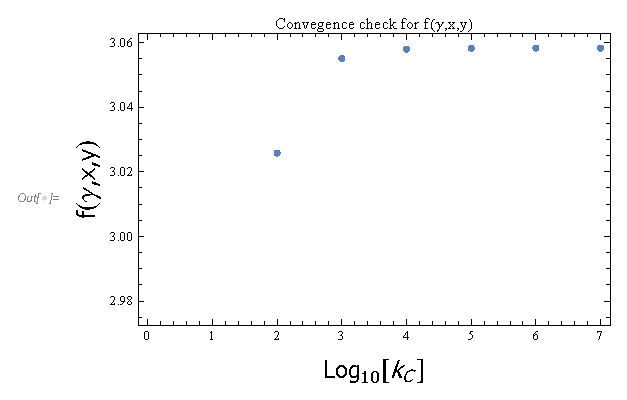
\includegraphics{Note_GPELAB_Droplet_gr1.eps}

We can say that integration up to order of 6 has converged. 
Then, we calculate \(f(\gamma ,x,y)\) with different \(x\), i.e. with different B-field Compared with Minardi{'}s approximation \cite{Minardi2019}, they propose a analytical approximation which will be more convenient for deriving GPE with LHY correction. Here is the formula:
\begin{equation}
\begin{split}
f(z,u=1,x)\simeq \left(1+z^{3/5}x\right)^{5/2}
\end{split}
\end{equation}
where
\begin{equation}
\begin{split}
z=m_2/m_1, x=\frac{g_{22}n_2}{g_{11}n_1},u=\frac{g_{12}^2}{g_{11}g_{22}}
\end{split}
\end{equation}

Here, \(u\) is set to be 1.
Now, we compare the numerical solution with the Minardi{'}s approximation.
Plot of List of f($\gamma $,x,y) for numerical one and Minardi{'}s approximation.

ADD FORMULAS

So, we can see that, there are mainly several percentage error by using this formula. And the maximum error is about 15$\%$. So, keep this error in mind about the LHY energy.

\section{Derivation of GPE and extendedGPE from mean-field energy}

First, we assume the many-body wave function is a product state

\begin{equation}
\begin{split}
\Psi \left(\overset{\rightharpoonup }{r}_1,\overset{\rightharpoonup }{r}_2,\ldots  ,\overset{\rightharpoonup }{r}_N\right)=\sum _{i=1}^N \psi \left(\overset{\rightharpoonup
}{r}_i\right)
\end{split}
\end{equation}

Then, we have

\begin{equation}
\begin{split}
E\left(\psi ,\psi ^*\right)=N\int dr^3\left(\frac{\hbar ^2}{2m}\left| \nabla \psi (r)\right| ^2+V(r)\left| \psi (r)\right| ^2+\frac{1}{2}N g\left|
\psi (r)\right| ^4\right)
\end{split}
\end{equation}

define the Variation

\begin{equation}
\begin{split}
X\left(\psi ,\psi ^*\right)=E\left(\psi ,\psi ^*\right)-\mu  N\int dr^3\left| \psi (r)\right| ^2
\end{split}
\end{equation}

take the variation of \(X\left(\psi ,\psi ^*\right)\), we have

\begin{equation}
\begin{split}
\delta  X\left(\psi ,\psi ^*\right)=N\int dr^3\left(\frac{\hbar ^2}{2m}\left(\nabla \psi ^*(r)\nabla \delta \psi (r)+\nabla \psi (r)\nabla \delta
\psi ^*(r)\right)+(V(r)-\mu )\left(\psi ^*(r)\delta  \psi (r)+\psi (r)\delta  \psi ^*(r) \right)+N g\left(\psi ^2(r)\delta  \psi ^*(r)+\psi ^*^2(r)\delta
 \psi (r)\right)\right)\\
=N\int dr^3\left(\frac{\hbar ^2}{2m}\left(\nabla \psi (r)\nabla \delta \psi ^*(r)\right)+(V(r)-\mu )\left(\psi (r)\delta  \psi ^*(r) \right)+N g\left(\psi
^2(r)\psi ^*(r)\delta  \psi ^*(r)\right)\right)+c.c.
\end{split}
\end{equation}

for the first part, by using integrating by part method:

\begin{equation}
\begin{split}
\int dr^3\left(\nabla \psi (r)\nabla \delta \psi ^*(r)\right)=\delta \psi ^*(r)\nabla \psi (r)|_0^{\infty }-\int dr^3\left(\nabla ^2\psi (r)\delta
\psi ^*(r)\right)=\int dr^3\left(-\nabla ^2\psi (r)\right)\delta \psi ^*(r)
\end{split}
\end{equation}

Them, take the variance to be zero, we have GPE

\begin{equation}
\begin{split}
-\frac{\hbar ^2}{2m}\left(\nabla ^2\psi (r)\right)+(V(r)-\mu )\psi (r)+N g\left(\psi ^2(r)\psi ^*(r)\right)=0\\
-\frac{\hbar ^2}{2m}\left(\nabla ^2\psi ^*(r)\right)+(V(r)-\mu )\psi ^*(r)+N g\left(\psi ^*^2(r)\psi (r)\right)=0
\end{split}
\end{equation}

First, we assume the many-body wave function is a product state

\begin{equation}
\begin{split}
\Psi \left(\overset{\rightharpoonup }{r}_1,\overset{\rightharpoonup }{r}_2,\ldots  ,\overset{\rightharpoonup }{r}_N\right)=\sum _{i=1}^N \psi \left(\overset{\rightharpoonup
}{r}_i\right)
\end{split}
\end{equation}

Then, we have

\begin{equation}
\begin{split}
E\left(\psi ,\psi ^*\right)=N\int dr^3\left(\frac{\hbar ^2}{2m}\left(\nabla \psi ^*(r)\nabla \psi (r)\right)+V(r)\left(\psi ^*(r)\psi (r)\right)+\frac{1}{2}N
g\left(\psi ^*(r)\psi (r)\right)^2+C \left(\psi ^*(r)\psi (r)\right)^{5/2}\right)
\end{split}
\end{equation}

define the Variation

\begin{equation}
\begin{split}
X\left(\psi ,\psi ^*\right)=E\left(\psi ,\psi ^*\right)-\mu  N\int dr^3\left(\psi ^*(r)\psi (r)\right)
\end{split}
\end{equation}

take the variation of \(X\left(\psi ,\psi ^*\right)\), we have

\begin{equation}
\begin{split}
\delta  X\left(\psi ,\psi ^*\right)=N\int dr^3\left(\frac{\hbar ^2}{2m}\left(\nabla ^2\psi (r)\delta \psi ^*(r)\right)+(V(r)-\mu )\left(\psi (r)\delta
\psi ^*(r) \right)+N g\left(\psi ^2(r)\psi ^*(r)\delta \psi ^*(r)\right)+\frac{5C}{2}(\psi (r))^{5/2}\left(\psi ^*(r)\right)^{3/2}\delta \psi ^*(r)\right)+c.c.
\end{split}
\end{equation}

where C is constants which already expressed the Last Part.
thus, we have eGPE

\begin{equation}
\begin{split}
-\frac{\hbar ^2}{2m}\left(\nabla ^2\psi (r)\right)+(V(r)-\mu )\psi (r)+N g\left(\psi ^*(r)\psi (r)\right)\psi (r)+\frac{5C}{2}\left(\psi (r)\psi
^*(r)\right)^{3/2}\psi (r)=0\\
-\frac{\hbar ^2}{2m}\left(\nabla ^2\psi ^*(r)\right)+(V(r)-\mu )\psi ^*(r)+N g\left(\psi ^*^2(r)\psi (r)\right)+\frac{5C}{2}\left(\psi ^*(r)\right)^{5/2}(\psi
(r))^{3/2}=0
\end{split}
\end{equation}

First, we assume the many-body wave function is a product state

\begin{equation}
\begin{split}
\Psi \left(\overset{\rightharpoonup }{r}_1,\overset{\rightharpoonup }{r}_2,\ldots  ,\overset{\rightharpoonup }{r}_N\right)=\sum _{i=1}^N \psi _1\left(\overset{\rightharpoonup
}{r}_i\right)\sum _{i=1}^N \psi _2\left(\overset{\rightharpoonup }{r}_i\right)
\end{split}
\end{equation}

Then, we have

\begin{equation}
\begin{split}
E\left(\psi _1,\psi _1{}^*,\psi _2,\psi _2{}^*\right)=\int dr^3\left(
\begin{array}{cc}
 \psi _1^* & \psi _2^* \\
\end{array}
\right).\left(
\begin{array}{cc}
 \mathcal{H}_{11} & \mathcal{H}_{12} \\
 \mathcal{H}_{21} & \mathcal{H}_{22} \\
\end{array}
\right).\left(
\begin{array}{c}
 \psi _1 \\
 \psi _2 \\
\end{array}
\right)+E_{\text{LHY}}
\end{split}
\end{equation}

where \(\mathcal{H}_{ij}\) represent the Hamiltonian density of fields

\begin{equation}
\begin{split}
\mathcal{H}_{11}=N_1\left(\frac{\hbar ^2}{2m_1}(\nabla )^2+V_1(r)+\frac{1}{2}N_1g_{11}\left(\psi _1{}^*(r)\psi _1(r)\right)\right)\\
\mathcal{H}_{22}=N_2\left(\frac{\hbar ^2}{2m_2}(\nabla )^2+V_2(r)+\frac{1}{2}N_2g_{22}\left(\psi _2{}^*(r)\psi _2(r)\right){}^2\right)\\
\mathcal{H}_{12}=\mathcal{H}_{21}^{\dagger }=N_1N_2g_{12}\left(\psi _1{}^*(r)\psi _1(r)\right)\left(\psi _2{}^*(r)\psi _2(r)\right)
\end{split}
\end{equation}

and LHY term has been expressed in the last part.
define the Variation

\begin{equation}
\begin{split}
X\left(\psi ,\psi ^*\right)=E\left(\psi ,\psi ^*\right)-\mu _1 N_1\int dr^3\left(\psi _1{}^*(r)\psi _1(r)\right)-\mu _2 N_2\int dr^3\left(\psi
_2{}^*(r)\psi _2(r)\right)
\end{split}
\end{equation}

Finally, we have eGPE for 

\begin{equation}
\begin{split}
i \hbar \frac{\partial \psi _1}{\partial t}=\left(-\frac{\hbar ^2\nabla ^2}{2m_1}+V_1+g_{11}n_1+g_{12}n_2+\frac{\delta  \mathcal{E}_{\text{LHY}}}{\delta
 n_1}\right)\psi _1\\
i \hbar \frac{\partial \psi _2}{\partial t}=\left(-\frac{\hbar ^2\nabla ^2}{2m_2}+V_2+g_{22}n_2+g_{12}n_1+\frac{\delta  \mathcal{E}_{\text{LHY}}}{\delta
 n_2}\right)\psi _2
\end{split}
\end{equation}

\section{eGPE for GPELAB with Minardi approximation}

\begin{equation}
\begin{split}
i \hbar \frac{\partial \psi _1}{\partial t}=\left(-\frac{\hbar ^2\nabla ^2}{2m_1}+V_1+g_{11}n_1+g_{12}n_2+\frac{\delta  \mathcal{E}_{\text{LHY}}}{\delta
 n_1}\right)\psi _1\\
i \hbar \frac{\partial \psi _2}{\partial t}=\left(-\frac{\hbar ^2\nabla ^2}{2m_2}+V_2+g_{22}n_2+g_{12}n_1+\frac{\delta  \mathcal{E}_{\text{LHY}}}{\delta
 n_2}\right)\psi _2
\end{split}
\end{equation}

where
\(n_i=N_i\psi _i^*\psi _i=N_i|\psi _i|^2\)
and 

\begin{equation}
\begin{split}
\frac{\delta  \mathcal{E}_{\text{LHY}}}{\delta  n_1}=\frac{8}{15\pi ^2}\frac{m_1^{3/2}\left(g_{11}\right){}^{5/2}n_1^{1/2}}{\hbar ^3}\left(\frac{5}{2}n_1f(\gamma
,x,y)-\frac{g_{22}n_2}{g_{11}}\frac{\partial f(\gamma ,x,y)}{\partial y}\right)
\end{split}
\end{equation}

\begin{equation}
\begin{split}
\frac{\delta  \mathcal{E}_{\text{LHY}}}{\delta  n_2}=\frac{8}{15\pi ^2}\frac{m_1^{3/2}\left(g_{11}\right){}^{3/2}g_{22}n_1^{3/2}}{\hbar ^3}\frac{\partial
f(\gamma ,x,y)}{\partial y}
\end{split}
\end{equation}

if we using the approximation formula, we have

\begin{equation}
\begin{split}
\mathcal{E}_{\text{LHY}}=\frac{8}{15\pi ^2}\frac{m_1^{3/2}\left(g_{11}n_1\right){}^{5/2}}{\hbar ^3}\left(1+\gamma ^{3/5}y\right)^{5/2}
\end{split}
\end{equation}

Then, 

\begin{equation}
\begin{split}
\frac{\delta  \mathcal{E}_{\text{LHY}}}{\delta  n_1}=\frac{8}{15\pi ^2}\frac{m_1^{3/2}\left(g_{11}\right){}^{5/2}n_1^{1/2}}{\hbar ^3}\left(\frac{5}{2}n_1\left(1+\gamma
^{3/5}y\right){}^{5/2}-\frac{5}{2}\frac{g_{22}n_2}{g_{11}}\left(1+\gamma ^{3/5}y\right)^{3/2}\gamma ^{3/5}\right)\\
=\frac{4}{3\pi ^2}\frac{m_1^{3/2}\left(g_{11}\right){}^{5/2}n_1^{3/2}}{\hbar ^3}\left(1+\gamma ^{3/5}y\right)^{3/2}
\end{split}
\end{equation}

\begin{equation}
\begin{split}
\frac{\delta  \mathcal{E}_{\text{LHY}}}{\delta  n_2}=\frac{8}{15\pi ^2}\frac{m_1^{3/2}\left(g_{11}\right){}^{3/2}g_{22}n_1^{3/2}}{\hbar ^3}\frac{5}{2}\left(1+\gamma
^{3/5}y\right)^{3/2}\gamma ^{3/5}\\
=\frac{4}{3\pi ^2}\frac{\gamma ^{3/5}m_1^{3/2}\left(g_{11}\right){}^{3/2}g_{22}n_1^{3/2}}{\hbar ^3}\left(1+\gamma ^{3/5}y\right)^{3/2}
\end{split}
\end{equation}

Finally, we have extended GPE as

\begin{equation}
\begin{split}
i \hbar \frac{\partial \psi _1}{\partial t}=\left(-\frac{\hbar ^2\nabla ^2}{2m_1}+V_1+g_{11}n_1+g_{12}n_2+\frac{4}{3\pi ^2}\frac{g_{11}m_1^{3/5}}{\hbar
^3}\left(g_{11}n_1m_1^{3/5}+g_{22}n_2m_2^{3/5}\right){}^{3/2}\right)\psi _1\\
i \hbar \frac{\partial \psi _2}{\partial t}=\left(-\frac{\hbar ^2\nabla ^2}{2m_2}+V_2+g_{22}n_2+g_{12}n_1+\frac{4}{3\pi ^2}\frac{g_{22}m_2^{3/5}}{\hbar
^3}\left(g_{11}n_1m_1^{3/5}+g_{22}n_2m_2^{3/5}\right){}^{3/2}\right)\psi _2
\end{split}
\end{equation}

Now, we need do DimensionReduction, 

\begin{equation}
\begin{split}
i \frac{\partial \Psi _1}{\partial T}=\left(-\frac{m\pmb{\nabla }^2}{2m_1}+\frac{V_1}{\hbar  \omega }+4\pi  \frac{m}{m_1}\frac{ N_1a_{11}}{a}\Psi
_1^*\Psi _1+2\pi \frac{ m }{m_{12}}\frac{N_2a_{12}}{a}\Psi _2^*\Psi _2+\frac{128\pi ^{1/2} }{3} \frac{a_{11}}{a}\left(\frac{m}{m_1}\right){}^{2/5}\left(
\frac{N_1a_{11}}{a}\left(\frac{m}{m_1}\right){}^{2/5}\Psi _1^*\Psi _1+ \frac{N_2a_{22}}{a}\left(\frac{m}{m_2}\right){}^{2/5}\Psi _2^*\Psi _2\right){}^{3/2}\right)\Psi
_1\\
i \frac{\partial \Psi _2}{\partial T}=\left(-\frac{m\pmb{\nabla }^2}{2m_2}+\frac{V_2}{\hbar  \omega }+4\pi  \frac{m}{m_2}\frac{\text{  }N_2a_{22}}{a}\Psi
_2^*\Psi _2+2\pi \frac{ m }{m_{12}}\frac{N_1a_{12}}{a}\Psi _1^*\Psi _1+\frac{128\pi ^{1/2} }{3}\frac{a_{22}}{a}\left(\frac{m}{m_2}\right){}^{2/5}\left(
\frac{N_1a_{11}}{a}\left(\frac{m}{m_1}\right){}^{2/5}\Psi _1^*\Psi _1+ \frac{N_2a_{22}}{a}\left(\frac{m}{m_2}\right){}^{2/5}\Psi _2^*\Psi _2\right){}^{3/2}\right)\Psi
_2
\end{split}
\end{equation}

where we set \(V_1\) and \(V_2\) as harmonic trap, and it gives the characteristic length and time. Actually, this characteristic length and time
can be arbitrary.

\begin{equation}
\begin{split}
g_{11}=\frac{4\pi  \hbar ^2a_{11}}{m_1}, g_{22}=\frac{4\pi  \hbar ^2a_{22}}{m_2}, g_{12}=\frac{2\pi  \hbar ^2a_{12}}{m_{12}}, m_{12}=\frac{m_1m_2}{m_1+m_2}\\
T=\omega  t, \overset{\rightharpoonup }{R}=\left.\overset{\rightharpoonup }{r}\right/a, \Psi =\psi  a^{3/2}, a=\sqrt{\frac{\hbar }{m \omega }}
\end{split}
\end{equation}

By the way, we can calculate the Nonlinear-Energy function. (Just for fun, not for GPELAB)

Recall LHY energy term

\begin{equation}
\begin{split}
\mathcal{E}_{\text{LHY}}=\frac{8}{15\pi ^2}\frac{m_1^{3/2}\left(g_{11}n_1\right){}^{5/2}}{\hbar ^3}\left(1+\left(\frac{m_2}{m_1}\right){}^{3/5}\frac{g_{22}n_2}{g_{11}n_1}\right){}^{5/2}\\
=\frac{256\sqrt{\pi }\hbar ^2}{15}\left(m_1^{-2/5}a_{11}n_1+m_2^{-2/5}a_{22}n_2\right){}^{5/2}
\end{split}
\end{equation}

Do DimensionReduction, we have

\begin{equation}
\begin{split}
\frac{\mathcal{E}_{\text{LHY}}}{\hbar  \omega \left/a^3\right.}=\frac{256\pi ^{1/2}}{15}\left(\frac{N_1a_{11}}{a}\left(\frac{m}{m_1}\right){}^{2/5}\Psi
_1^*\Psi _1+ \frac{N_2a_{22}}{a}\left(\frac{m}{m_2}\right){}^{2/5}\Psi _2^*\Psi _2\right){}^{5/2}
\end{split}
\end{equation}

%\input{sections/S3_MOLSCAT}
\chapter{Camera comparison and absorption image SNR analysis}

\section{Absorption SNR analysis}

When doing absorption image, we typically take three images, noted as:
\begin{itemize}[noitemsep,topsep=0pt]
    \item \(C_{\text{in}}(x,y)\) as input light distribution on the atom
    \item \(C_{\text{out}}(x,y)\) as output(after absorption) light
    \item \(C_{\text{bg}}(x,y)\) as the background
\end{itemize}
formula of OD is
\begin{equation}
\text{OD}(x,y)=n_{\text{col}}(x,y)\sigma _0^*=\text{Log}\left[\frac{C_{\text{in}}(x,y)-C_{\text{bg}}(x,y)}{C_{\text{out}}(x,y)-C_{\text{bg}}(x,y)}\right]+\frac{C_{\text{in}}(x,y)-C_{\text{out}}(x,y)}{C_{\text{sat}}^{\text{eff}}}
\end{equation}
where
\begin{itemize}[noitemsep,topsep=0pt]
    \item \(C(x,y)=I(x,y)\times \frac{A_{\text{pix}}}{M^2}\times \frac{\lambda }{h c}\times T\times \text{QE}\times \tau \times \frac{1}{\text{ADC}}\)
    \item \(I(x,y)\) is the intensity distribution of light on atom
    \item \(A_{\text{pix}}\) is the pixel size of camera, \(\frac{A_{\text{pix}}}{M^2}\) is the real pixel size with counting magnification of image system.
    \item $\lambda $ is the probe light wavelength
    \item T is the transmission rate of the image system
    \item QE is the quantum efficiency of the camera
    \item ADC is the ADC conversion efficiency of the camera
    \item $\tau $ is the exposure time
\end{itemize}

The Noise is
\begin{equation}
\begin{split}
\sigma _{\text{OD}}^2&=\left(\frac{\partial \text{OD}}{\partial C_{\text{in}}}\right){}^2\sigma _{C_{\text{in}}}^2+\left(\frac{\partial \text{OD}}{\partial C_{\text{out}}}\right){}^2\sigma _{C_{\text{out}}}^2+\left(\frac{\partial \text{OD}}{\partial C_{\text{bg}}}\right){}^2\sigma _{C_{\text{bg}}}^2\\
&=\left(\frac{1}{C_{\text{sat}}^{\text{eff}}}+\frac{1}{C_{\text{in}}-C_{\text{bg}}}\right){}^2\sigma _{C_{\text{in}}}^2+\left(\frac{1}{C_{\text{sat}}^{\text{eff}}}+\frac{1}{C_{\text{out}}-C_{\text{bg}}}\right){}^2\sigma_{C_{\text{out}}}^2\\
&+\left(\frac{1}{C_{\text{in}}-C_{\text{bg}}}-\frac{1}{C_{\text{out}}-C_{\text{bg}}}\right){}^2\sigma _{C_{\text{bg}}}^2
\end{split}
\end{equation}

Then, The Signal to Noise ratio is
\begin{equation}
\begin{split}
\text{SNR}&=\frac{\text{Log}\left[\frac{C_{\text{in}}-C_{\text{bg}}}{C_{\text{out}}-C_{\text{bg}}}\right]+\frac{C_{\text{in}}-C_{\text{out}}}{C_{\text{sat}}^{\text{eff}}}}{\sqrt{\alpha^2+\beta^2+\gamma^2}}\\
\alpha^2&=\left(\frac{1}{C_{\text{sat}}^{\text{eff}}}+\frac{1}{C_{\text{in}}-C_{\text{bg}}}\right){}^2\sigma_{C_{\text{in}}}^2\\
\beta^2&=\left(\frac{1}{C_{\text{sat}}^{\text{eff}}}+\frac{1}{C_{\text{out}}-C_{\text{bg}}}\right){}^2\sigma _{C_{\text{out}}}^2\\
\gamma^2&=\left(\frac{1}{C_{\text{in}}-C_{\text{bg}}}-\frac{1}{C_{\text{out}}-C_{\text{bg}}}\right){}^2\sigma
_{C_{\text{bg}}}^2
\end{split}
\end{equation}

Put noise formula into the above SNR, we have

\begin{equation}
\begin{split}
\text{SNR}&=\frac{\text{Log}\left[\frac{C_{\text{in}}-C_{\text{bg}}}{C_{\text{out}}-C_{\text{bg}}}\right]+\frac{C_{\text{in}}-C_{\text{out}}}{C_{\text{sat}}^{\text{eff}}}}{\sqrt{X^2+Y^2+Z^2+W^2}}\\
X^2&=\left[\left(\frac{1}{C_{\text{sat}}^{\text{eff}}}+\frac{1}{C_{\text{in}}-C_{\text{bg}}}\right){}^2+\left(\frac{1}{C_{\text{sat}}^{\text{eff}}}+\frac{1}{C_{\text{out}}-C_{\text{bg}}}\right){}^2\right.\\
&\left.+\left(\frac{1}{C_{\text{in}}-C_{\text{bg}}}-\frac{1}{C_{\text{out}}-C_{\text{bg}}}\right){}^2\right]\sigma_{\text{readout}}^2\\
Y^2&=\left(\frac{1}{C_{\text{sat}}^{\text{eff}}}+\frac{1}{C_{\text{in}}-C_{\text{bg}}}\right){}^2\sigma _{\text{in}-\text{signal}}^2\\
Z^2&=\left(\frac{1}{C_{\text{sat}}^{\text{eff}}}+\frac{1}{C_{\text{out}}-C_{\text{bg}}}\right){}^2\sigma_{\text{out}-\text{signal}}^2\\
W^2&=\left(\frac{1}{C_{\text{in}}-C_{\text{bg}}}-\frac{1}{C_{\text{out}}-C_{\text{bg}}}\right){}^2\sigma _{\text{bg}-\text{signal}}^2
\end{split}
\end{equation}

\begin{table}[hbt]
\caption[Cameras parameter table]{Camera parameter table}
\label{camera_test}
\begin{tabular}{|l|l|l|l|l|}
\hline
                                                                               & PCO-Pixelfly & GS3-U3-15S5M-C & BFS-PGE-31S4 & PCO-sCOS \\ \hline
Wavelength(nm)                                                                 & 589/780      & 589/780        & 589/780      & 589/780  \\ \hline
QE(\%) on datasheet                                                            & 58/25        & 72/35          & 70/30        & 61/35    \\ \hline
QE(\%) measured                                                                & -/22.0       & 56.6/-         & 47.2/27.0    &          \\ \hline
\begin{tabular}[c]{@{}l@{}}Readout noise(e)\\ on datasheet\end{tabular}        & 6            & 8.31           & 2.29         & 1.1      \\ \hline
\begin{tabular}[c]{@{}l@{}}Readout noise(e)\\ measured\end{tabular}            &              &                & 0.53         &          \\ \hline
\begin{tabular}[c]{@{}l@{}}Dark noise rate\\ on datasheet\end{tabular}         & 1 e/s        &                &              & 0.8 e/s  \\ \hline
\begin{tabular}[c]{@{}l@{}}Dark noise rate\\ measured\end{tabular}             &              &                & 0.59 e/s     &          \\ \hline
\begin{tabular}[c]{@{}l@{}}A/D conversion(e/count)\\ on datasheet\end{tabular} & 1            & tunable        & tunable      & 0.46     \\ \hline
\begin{tabular}[c]{@{}l@{}}A/D conversion(e/count)\\ measured\end{tabular}     &              &                & 1/0.53       &          \\ \hline
\end{tabular}
\end{table}
\newpage
\setstretch{1}
\bibliography{database}
%=======================================================
\end{document}